\chapter{RHC Multi Pi Samples Validation}\label{appendix:rhcmpi}

Various fits were run to validate the implementation of the RHC samples being divided by $\pi$ rather than track multiplicity. Data fits using only runs 2-4 and 8 were run, as the FHC sample should be unaffected by the changes. The results are shown in Figures \ref{fig:rhcmpidat248fluxSK} and \ref{fig:rhcmpidat248xsec}, and as expected, there is no difference using the RHC multi-$\pi$ or RHC multi-track sample implementations. 

\begin{figure}[t]
\centering
\begin{subfigure}{0.95\textwidth}
  \centering
  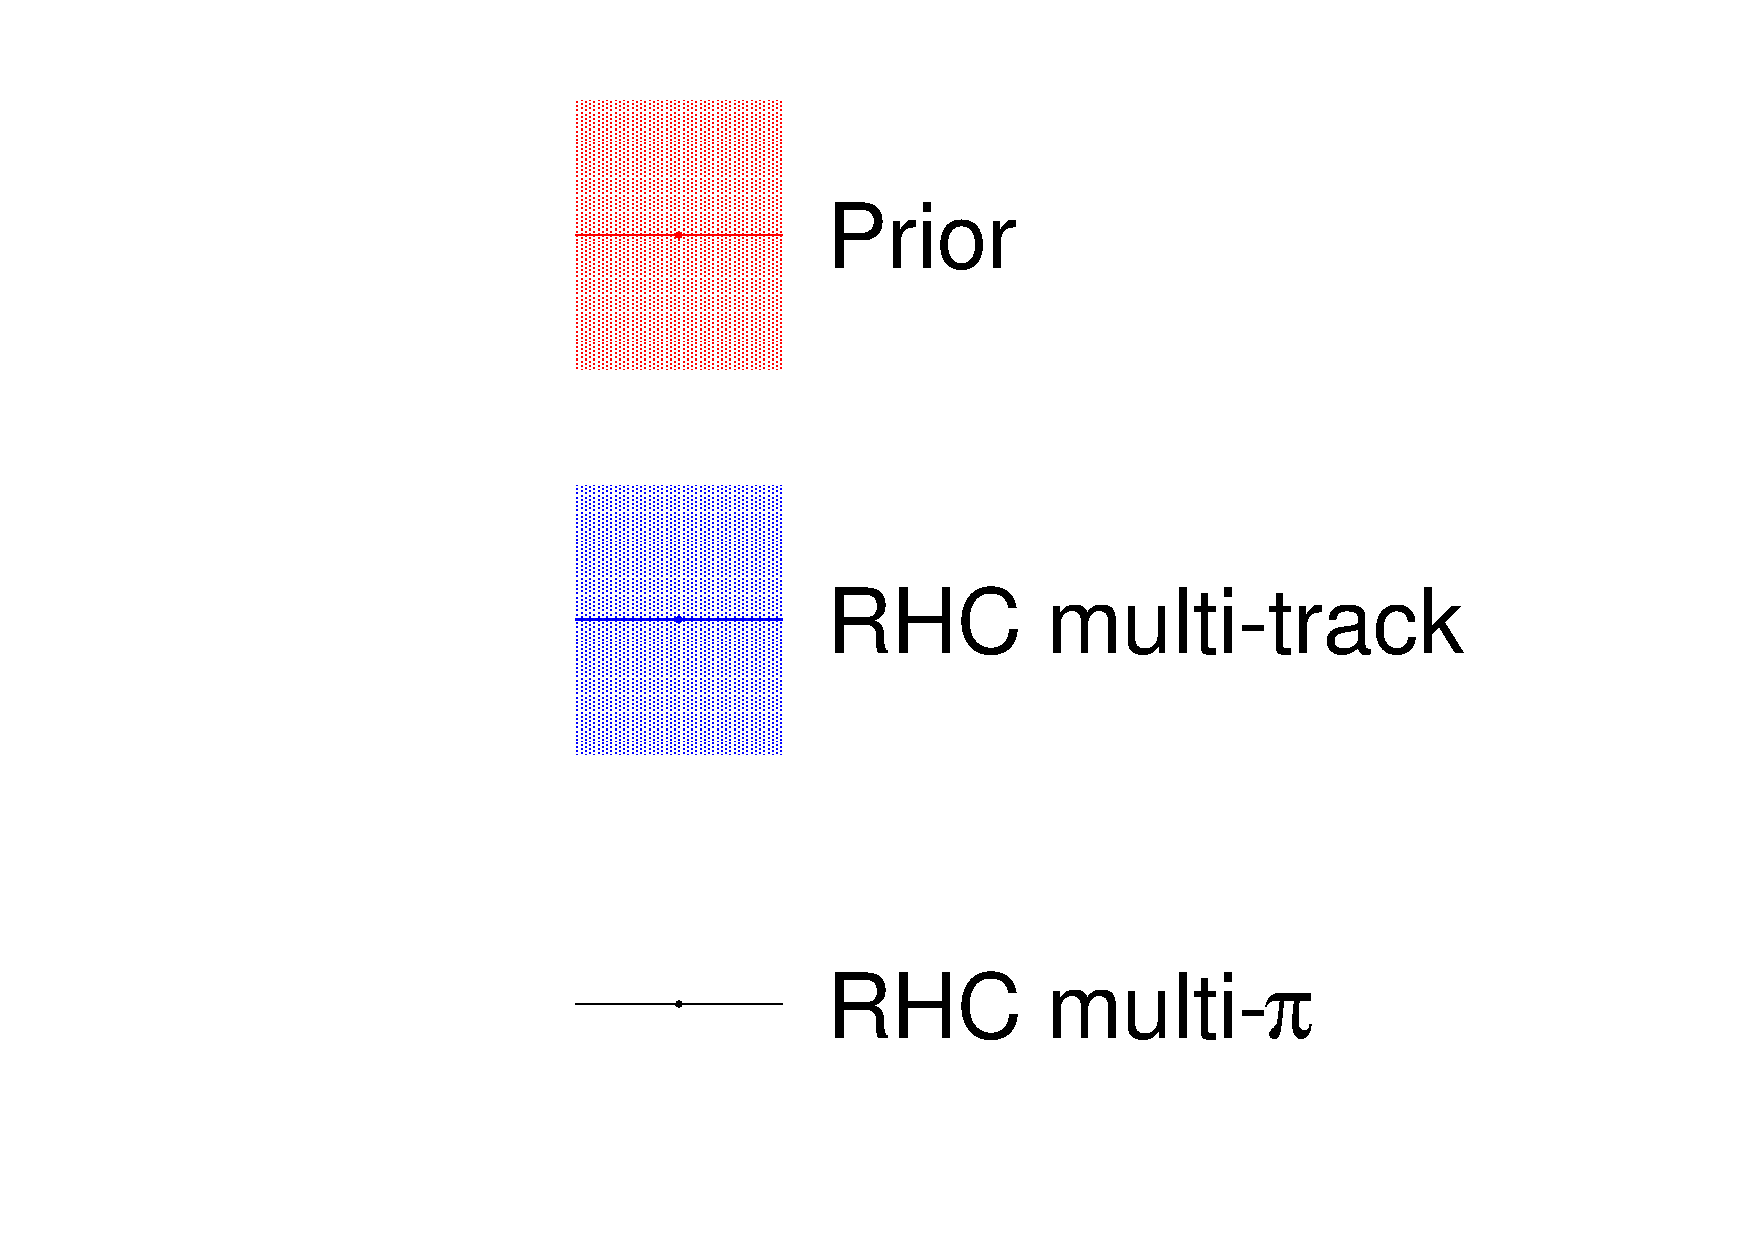
\includegraphics[width=0.24\linewidth]{figs/rhcmpdat248_leg}	
\end{subfigure}
\begin{subfigure}{0.24\textwidth}
  \centering
  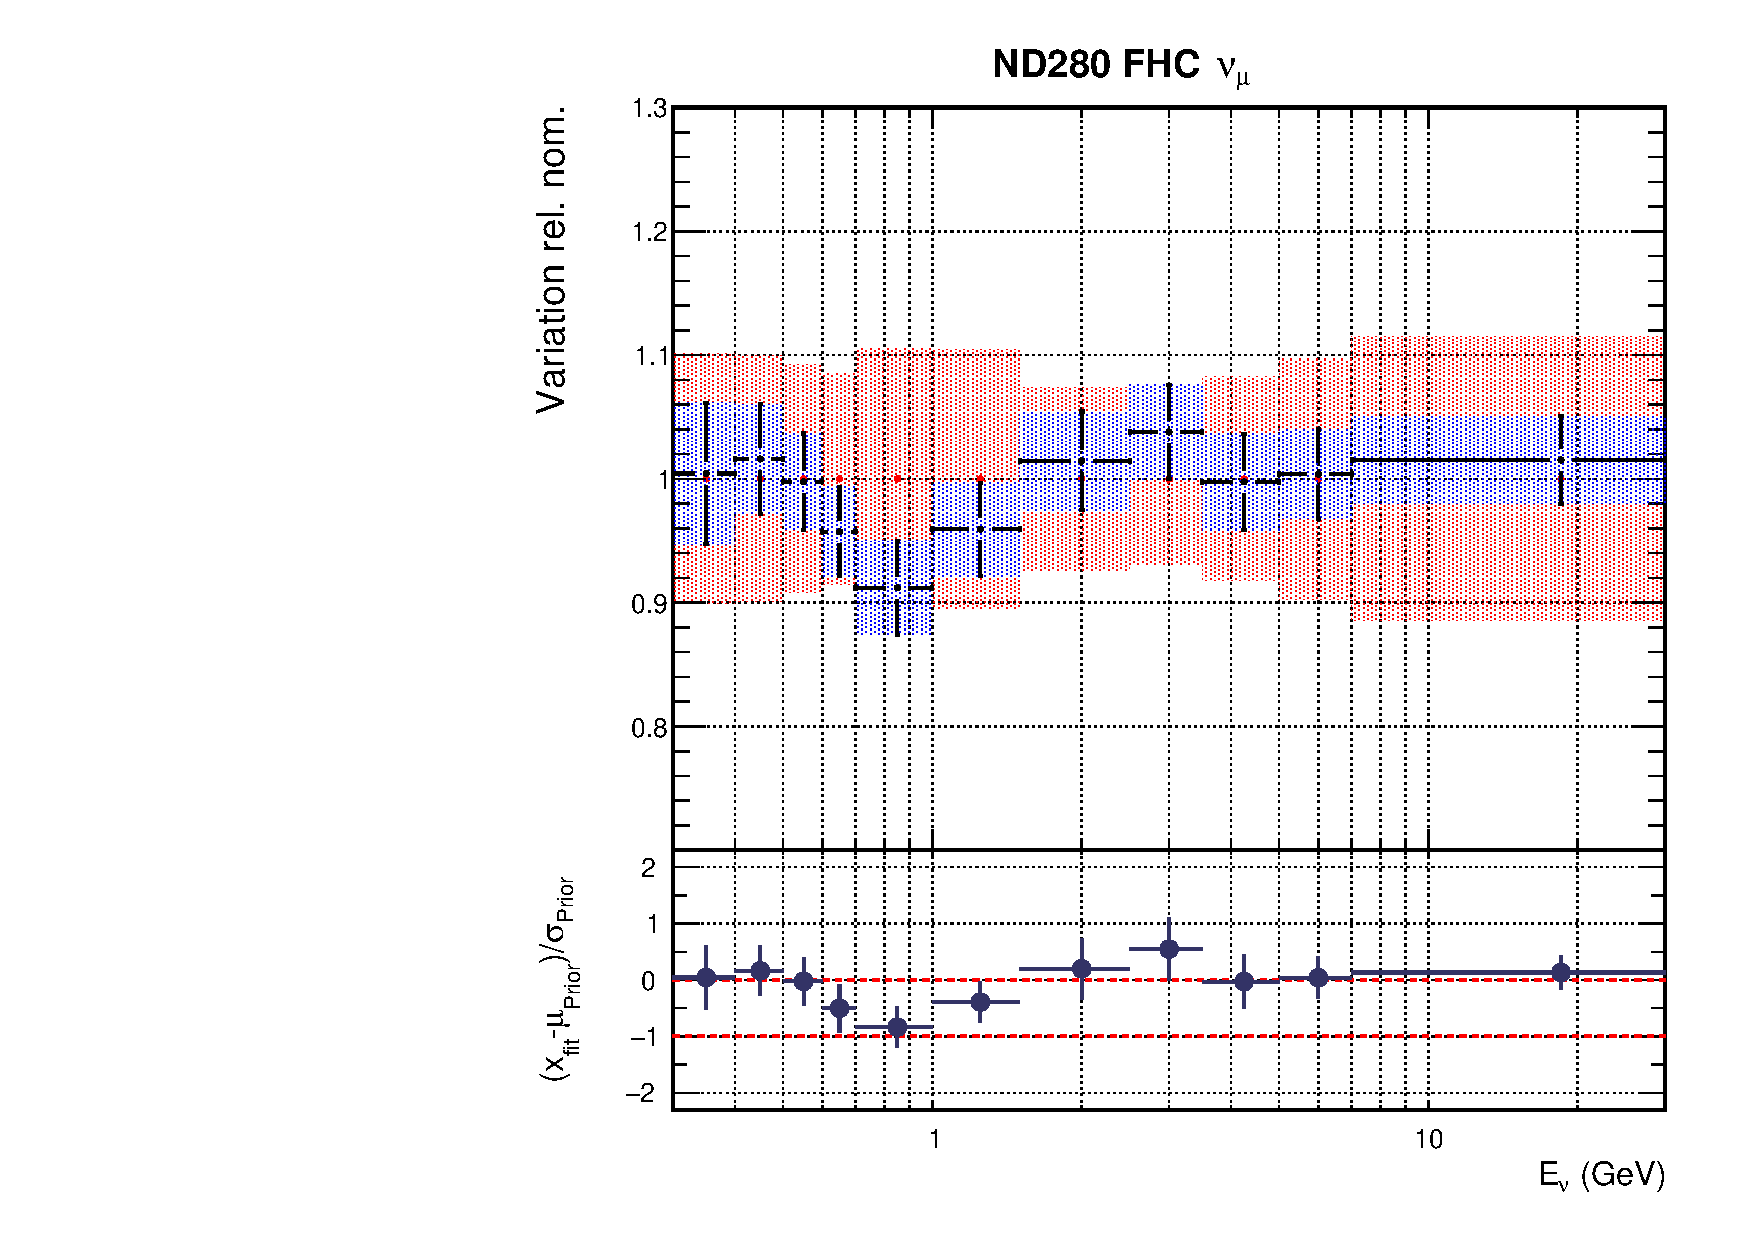
\includegraphics[width=0.95\linewidth]{figs/rhcmpdat248flux_0}
  \caption{ND FHC $\nu_{\mu}$}
\end{subfigure}
\begin{subfigure}{0.24\textwidth}
  \centering
  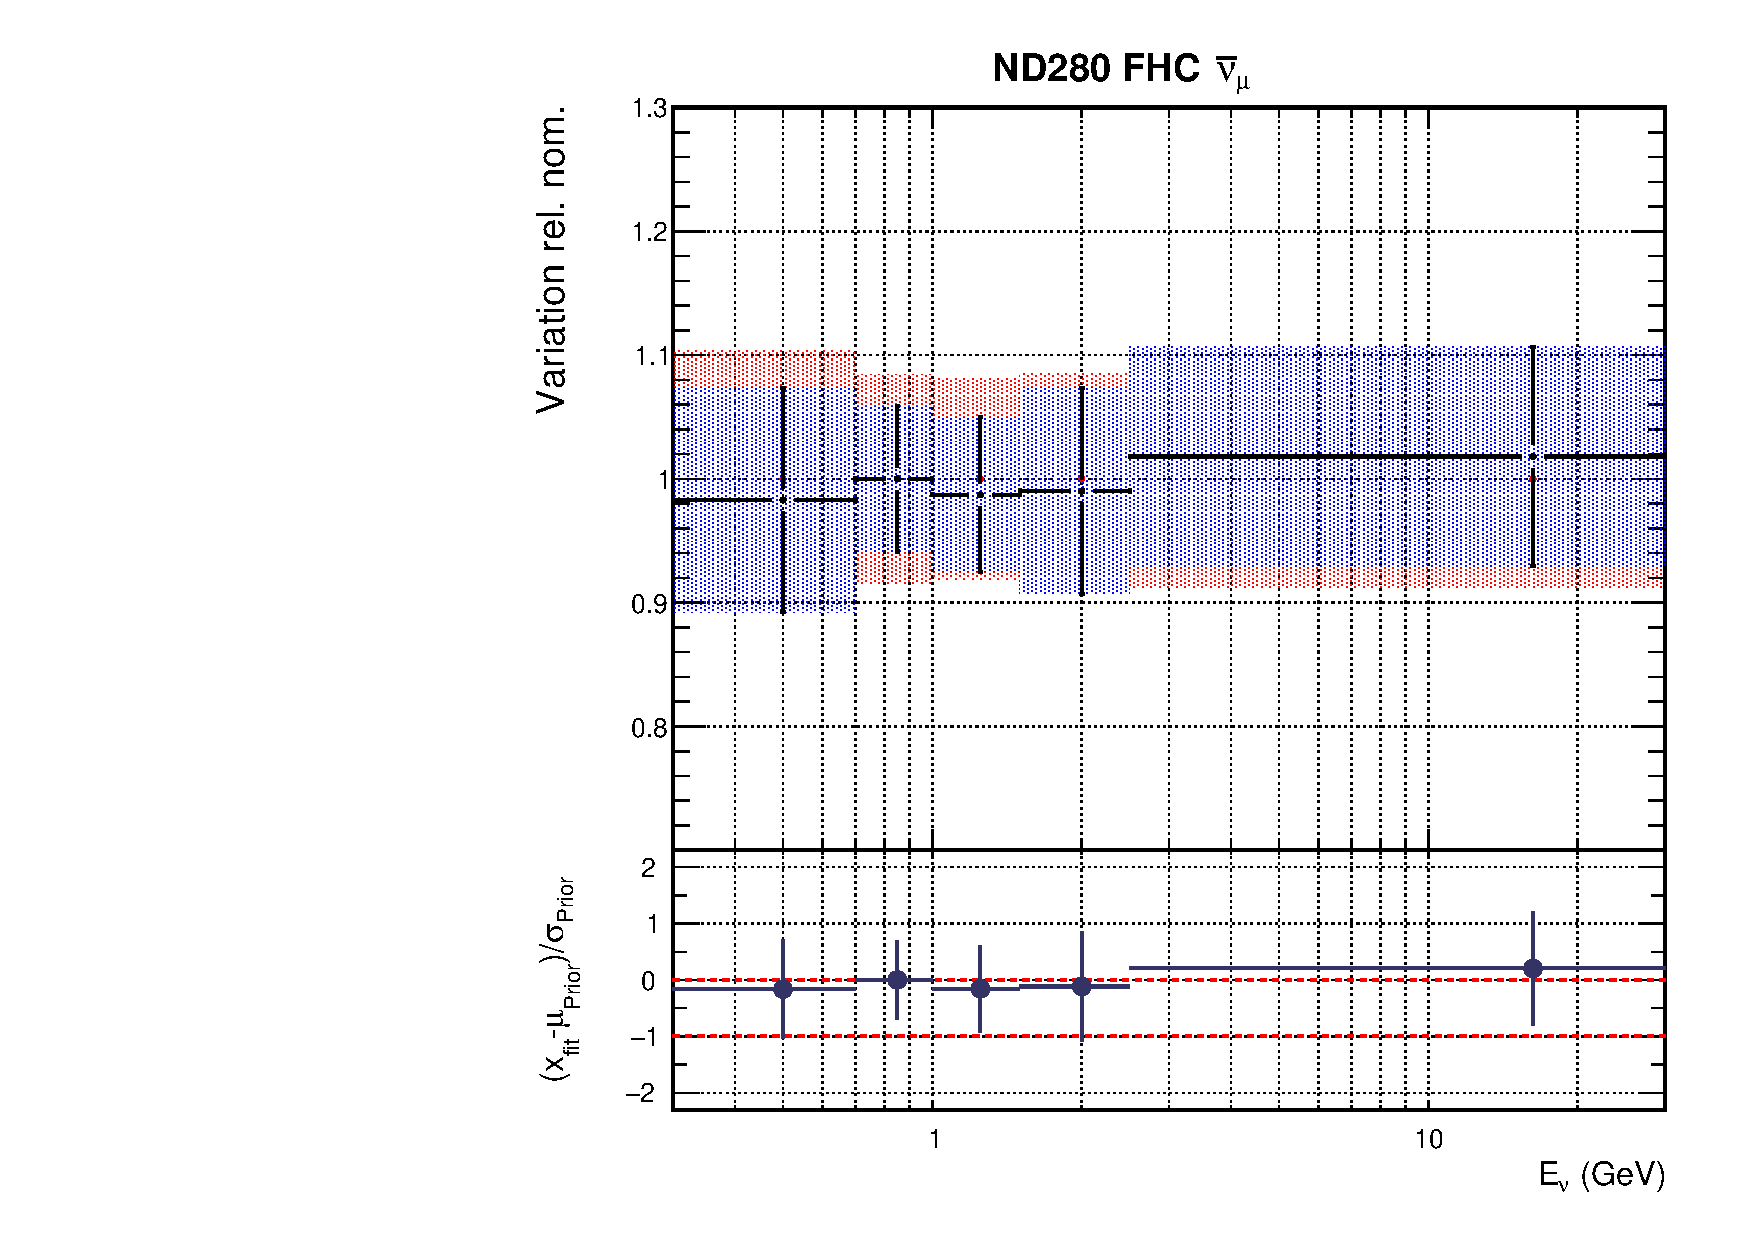
\includegraphics[width=0.95\linewidth]{figs/rhcmpdat248flux_1}
  \caption{ND FHC $\nu_e$}
\end{subfigure}
\begin{subfigure}{0.24\textwidth}
  \centering
  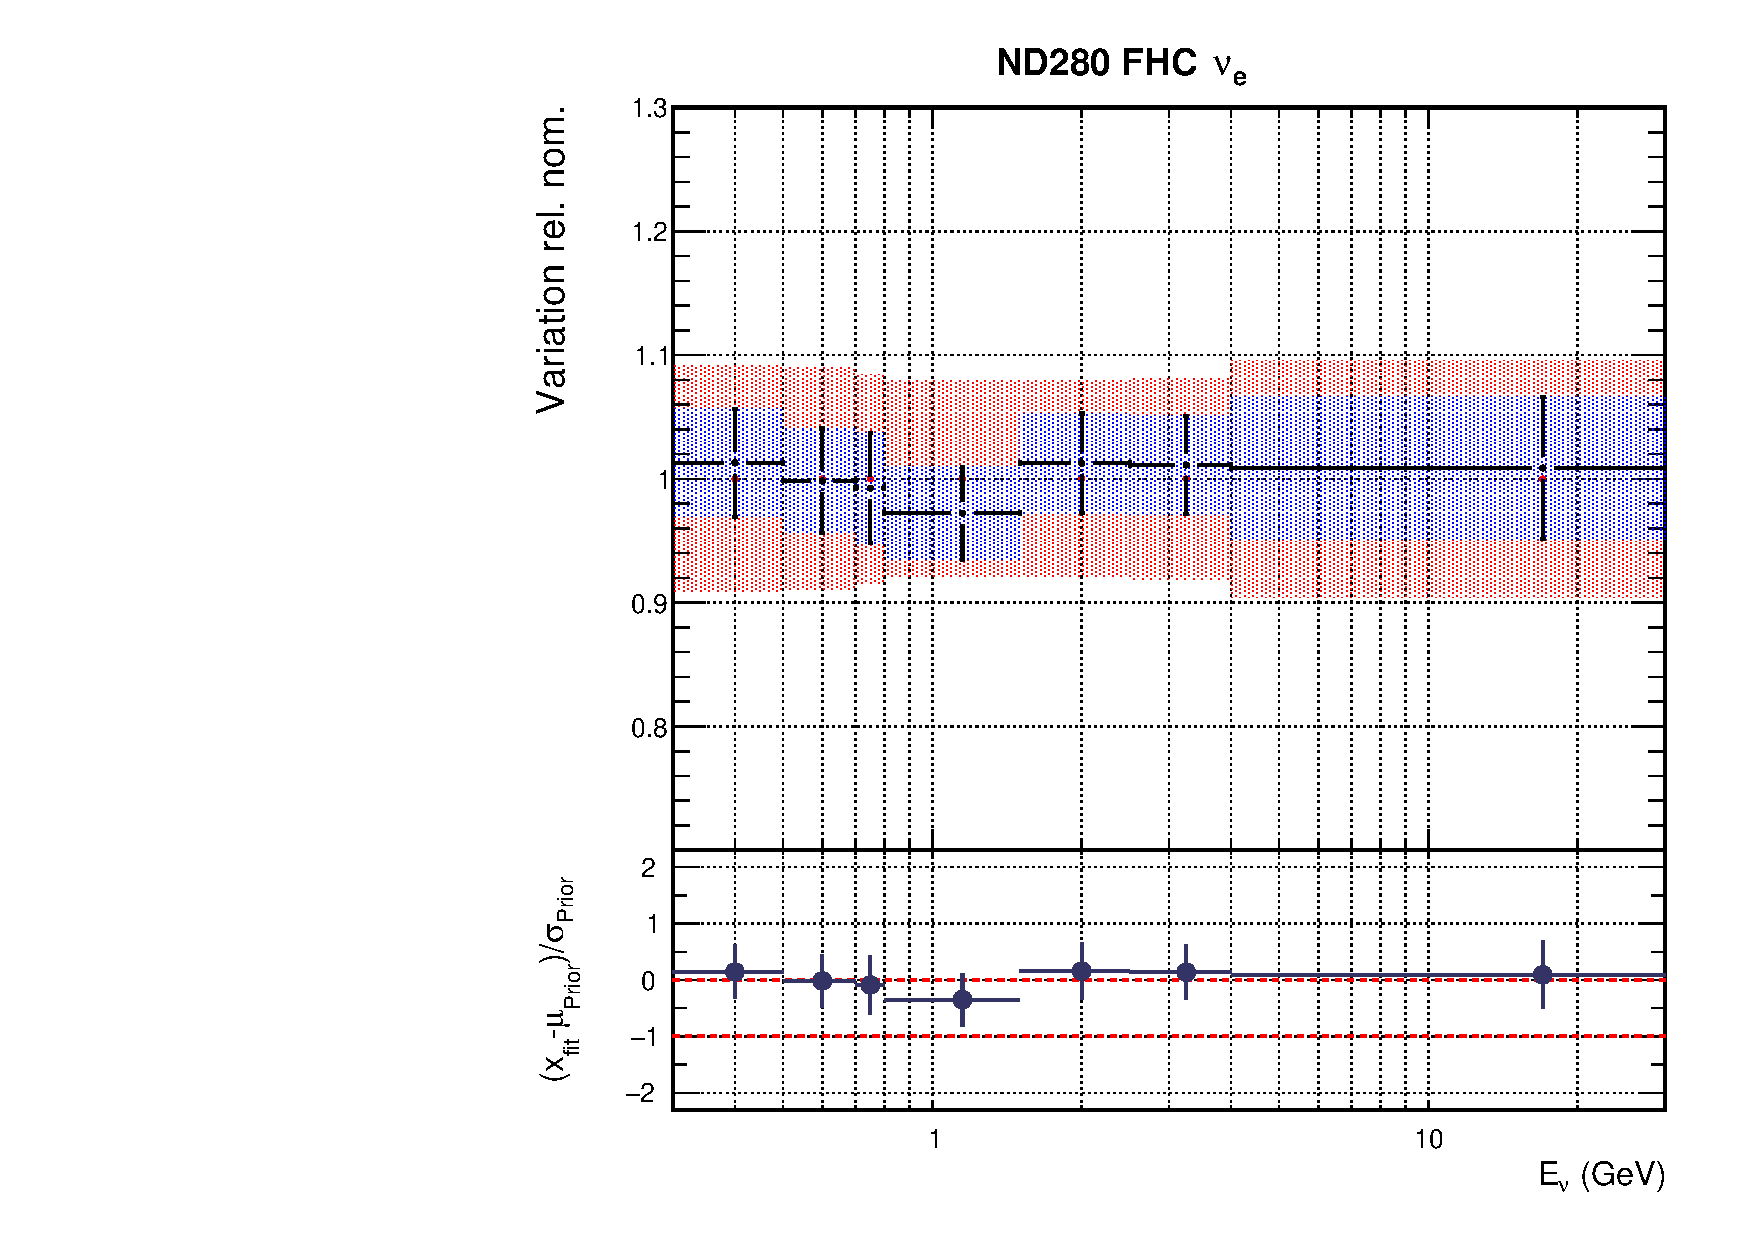
\includegraphics[width=0.95\linewidth]{figs/rhcmpdat248flux_2}
  \caption{ND FHC $\bar{\nu_{\mu}}$}
\end{subfigure}
\begin{subfigure}{0.24\textwidth}
  \centering
  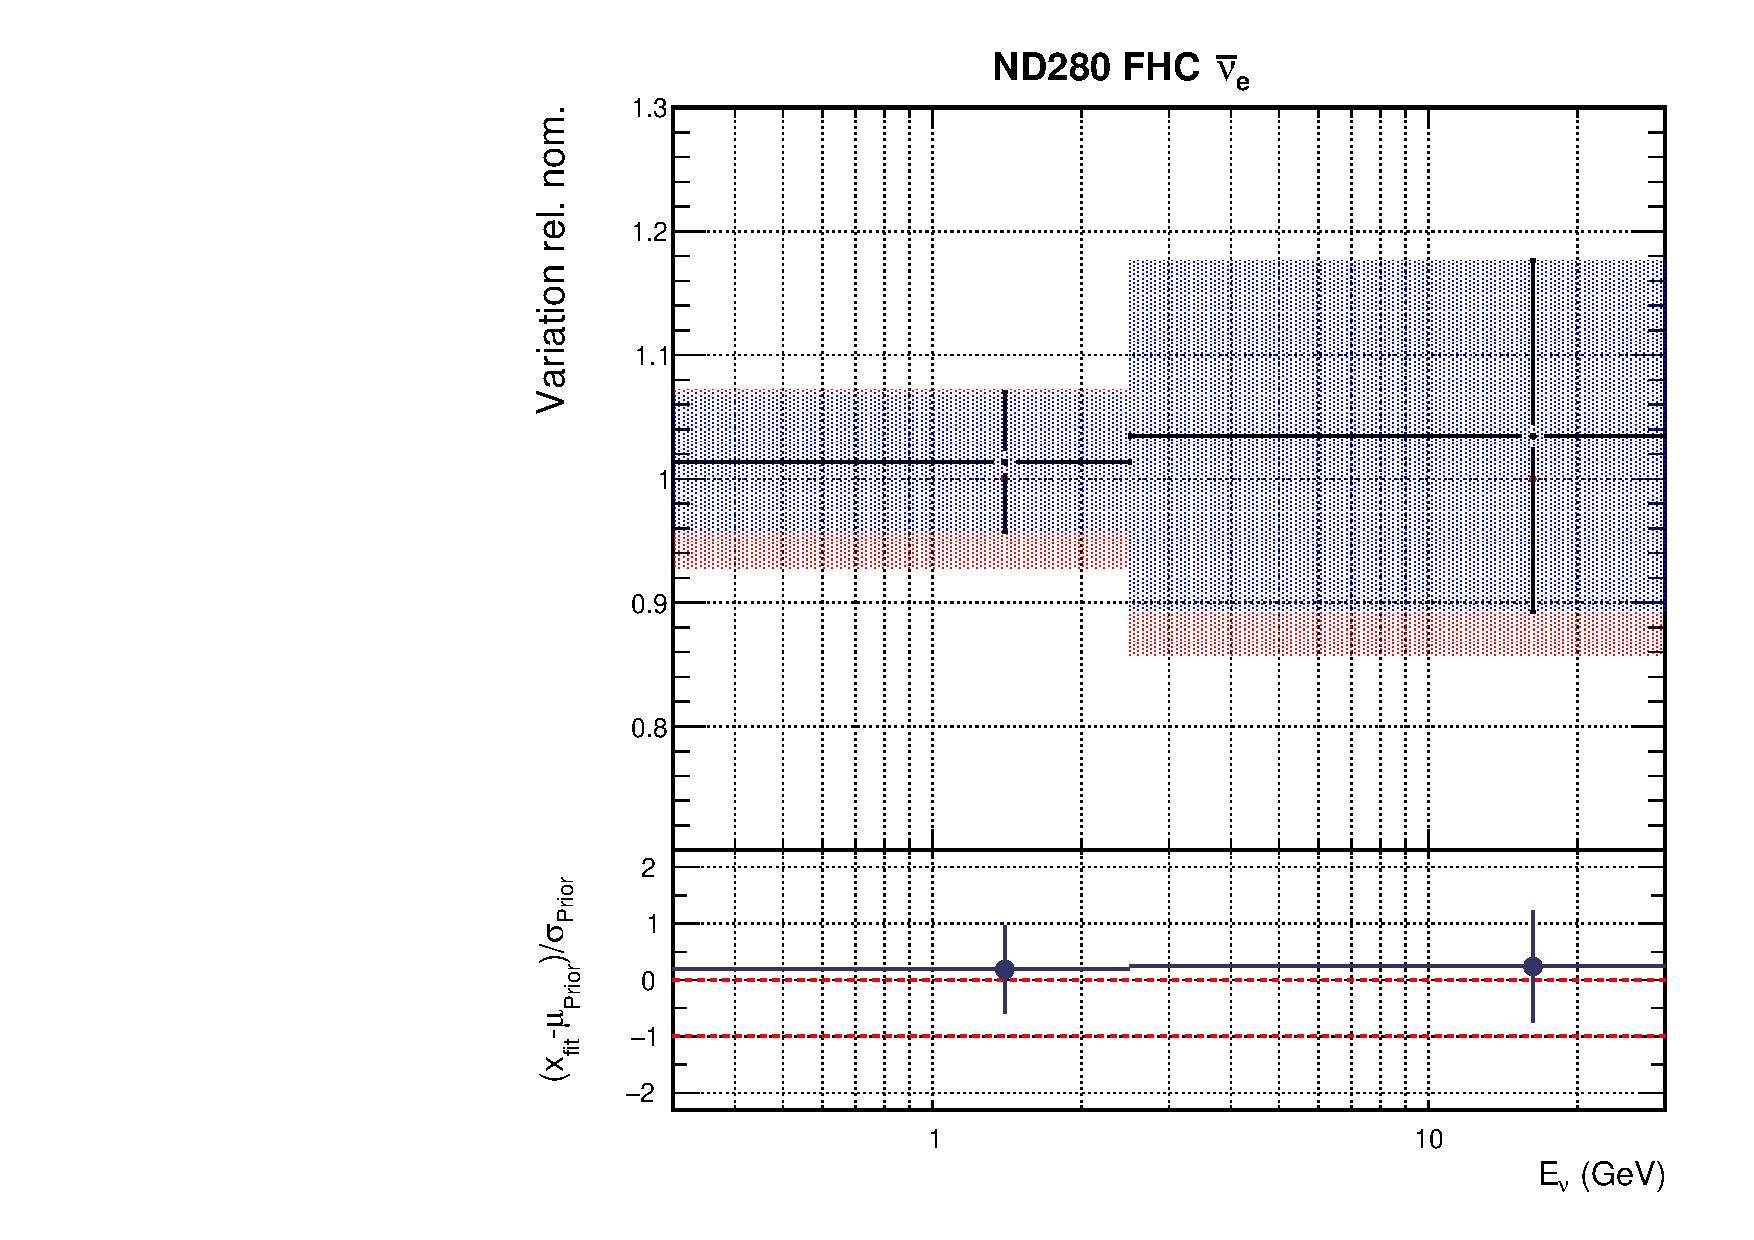
\includegraphics[width=0.95\linewidth]{figs/rhcmpdat248flux_3}
  \caption{ND FHC $\bar{\nu_{e}}$}
\end{subfigure}
\begin{subfigure}{0.24\textwidth}
  \centering
  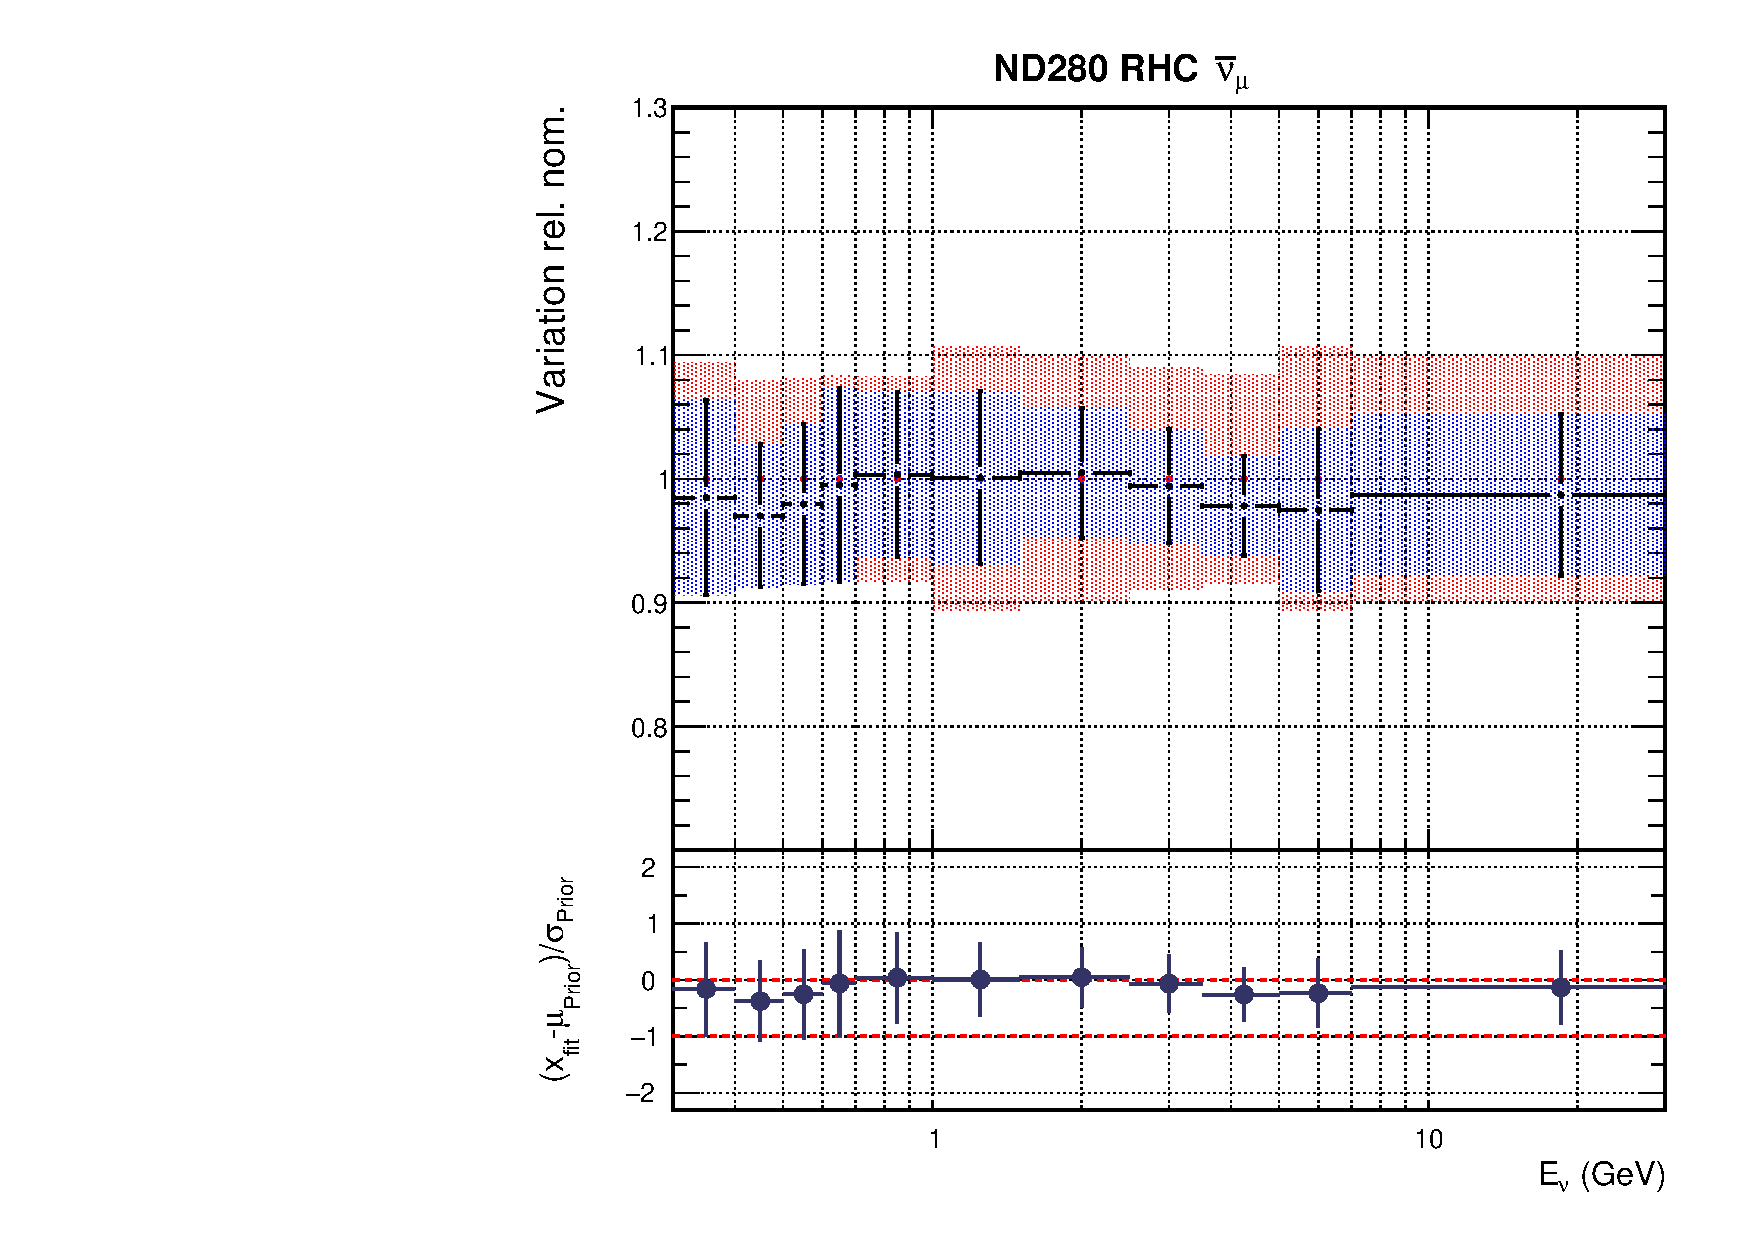
\includegraphics[width=0.95\linewidth]{figs/rhcmpdat248flux_4}
  \caption{ND RHC $\bar{\nu_{\mu}}$}
\end{subfigure}
\begin{subfigure}{0.24\textwidth}
  \centering
  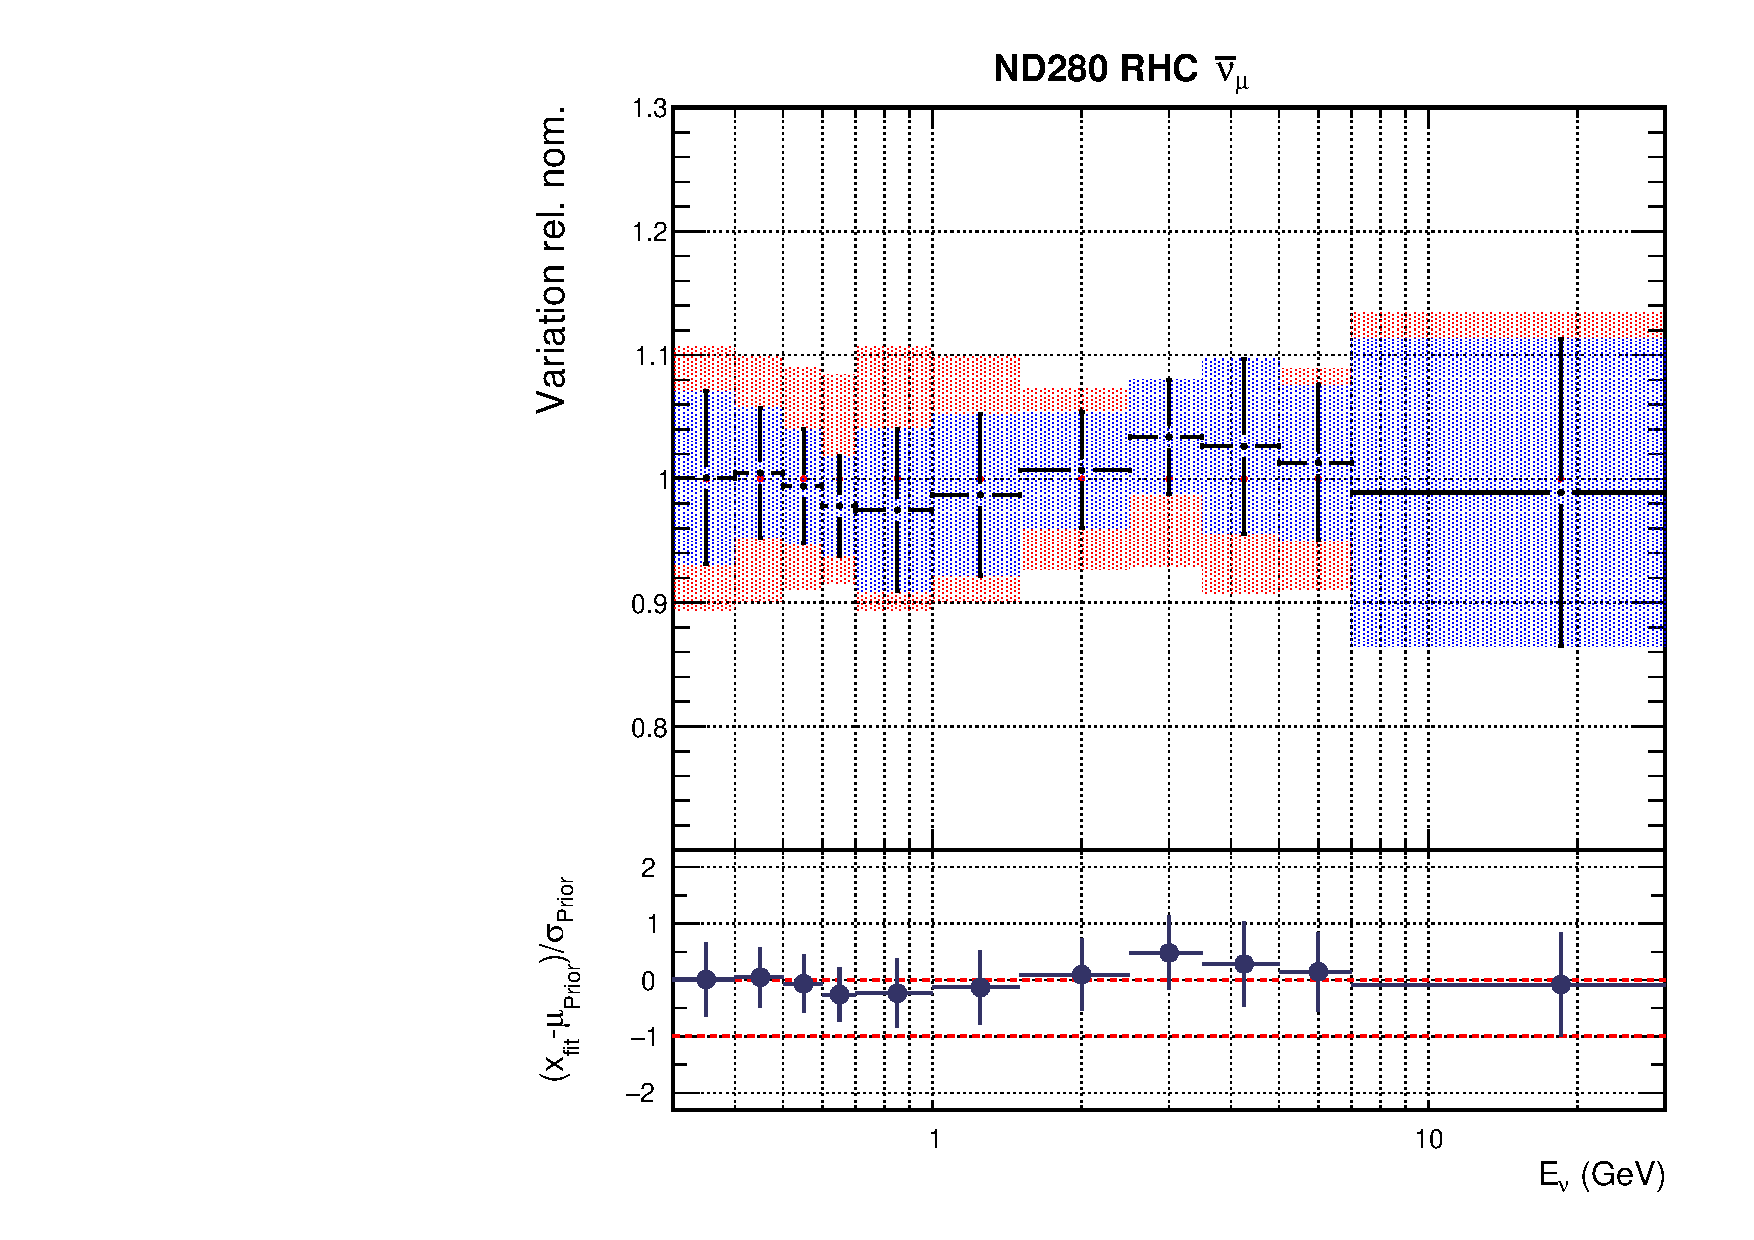
\includegraphics[width=0.95\linewidth]{figs/rhcmpdat248flux_5}
  \caption{ND RHC $\bar{\nu_{e}}$}
\end{subfigure}
\begin{subfigure}{0.24\textwidth}
  \centering
  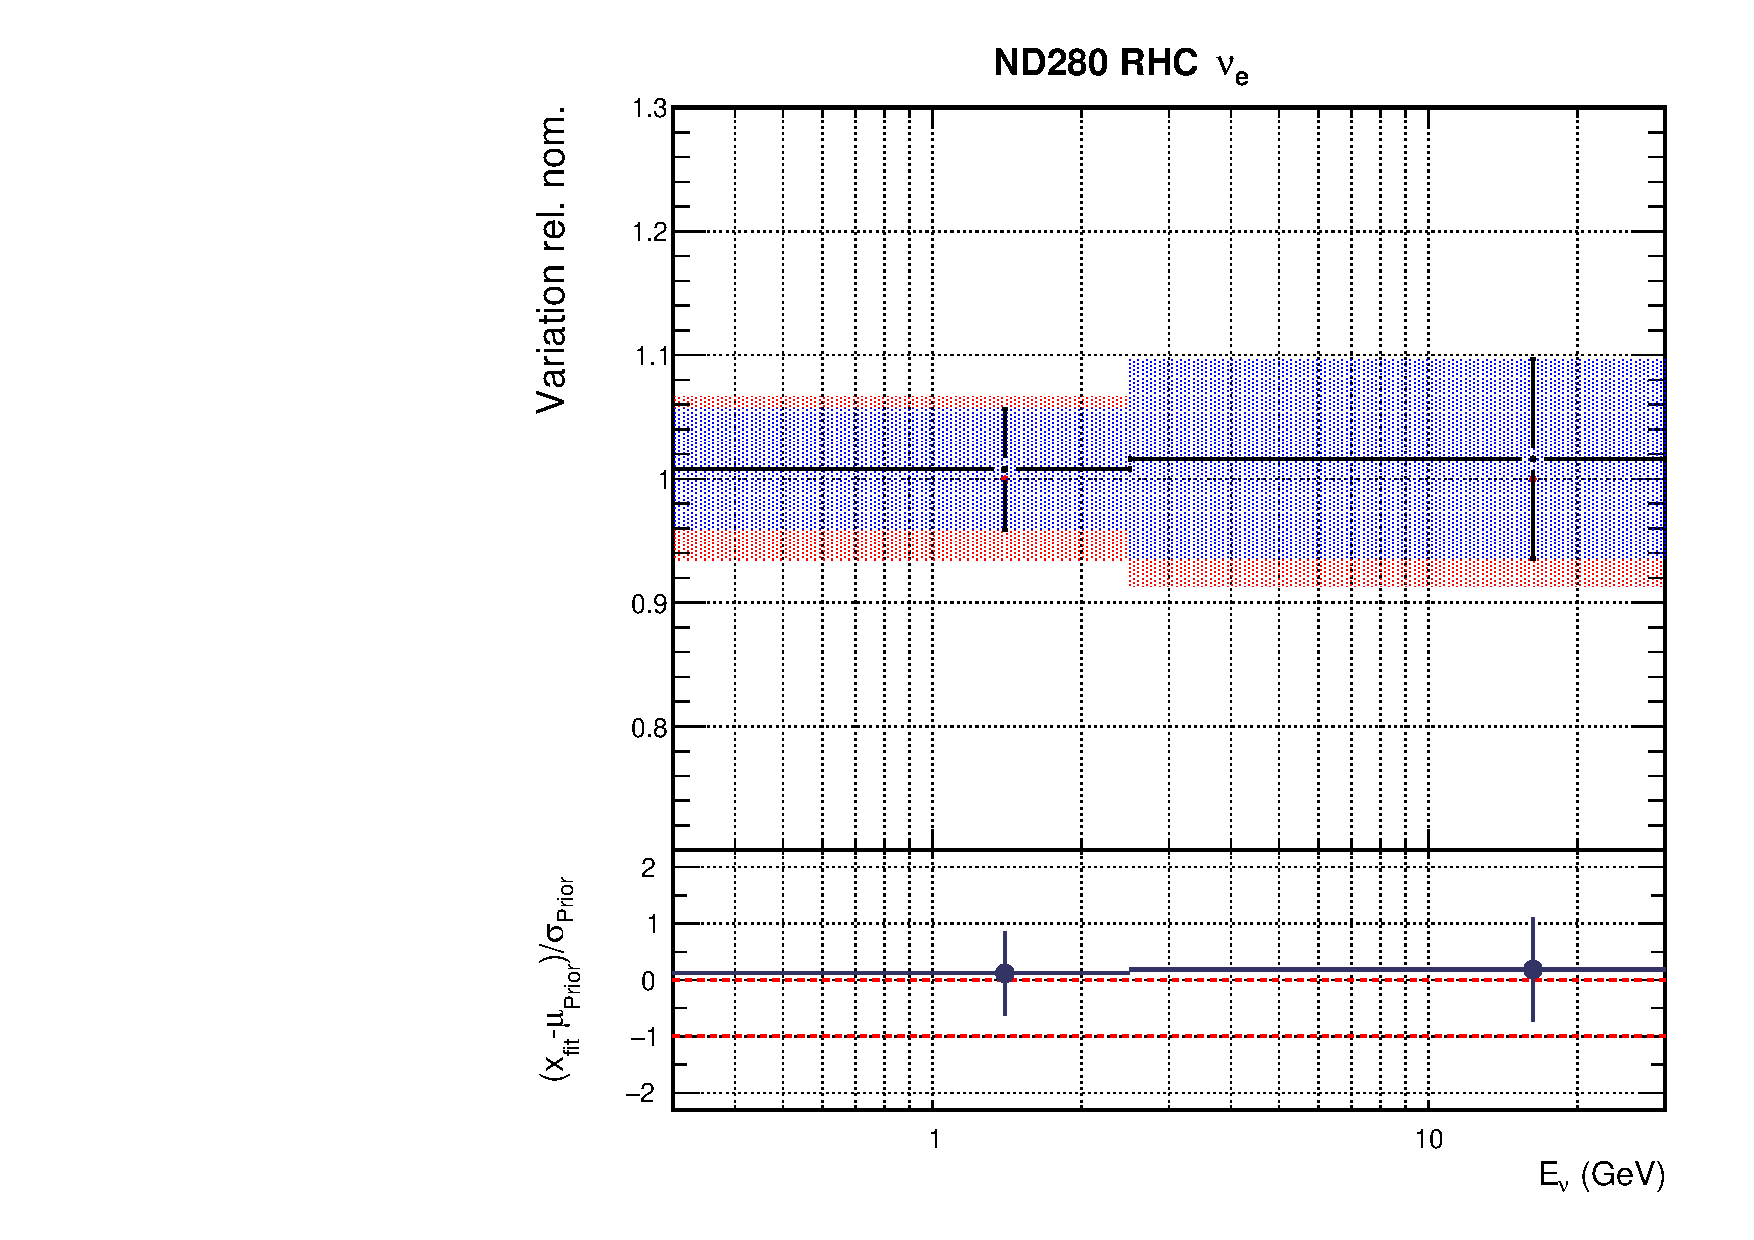
\includegraphics[width=0.95\linewidth]{figs/rhcmpdat248flux_6}
  \caption{ND RHC $\nu_{\mu}$}
\end{subfigure}
\vspace{15mm}
\begin{subfigure}{0.24\textwidth}
  \centering
  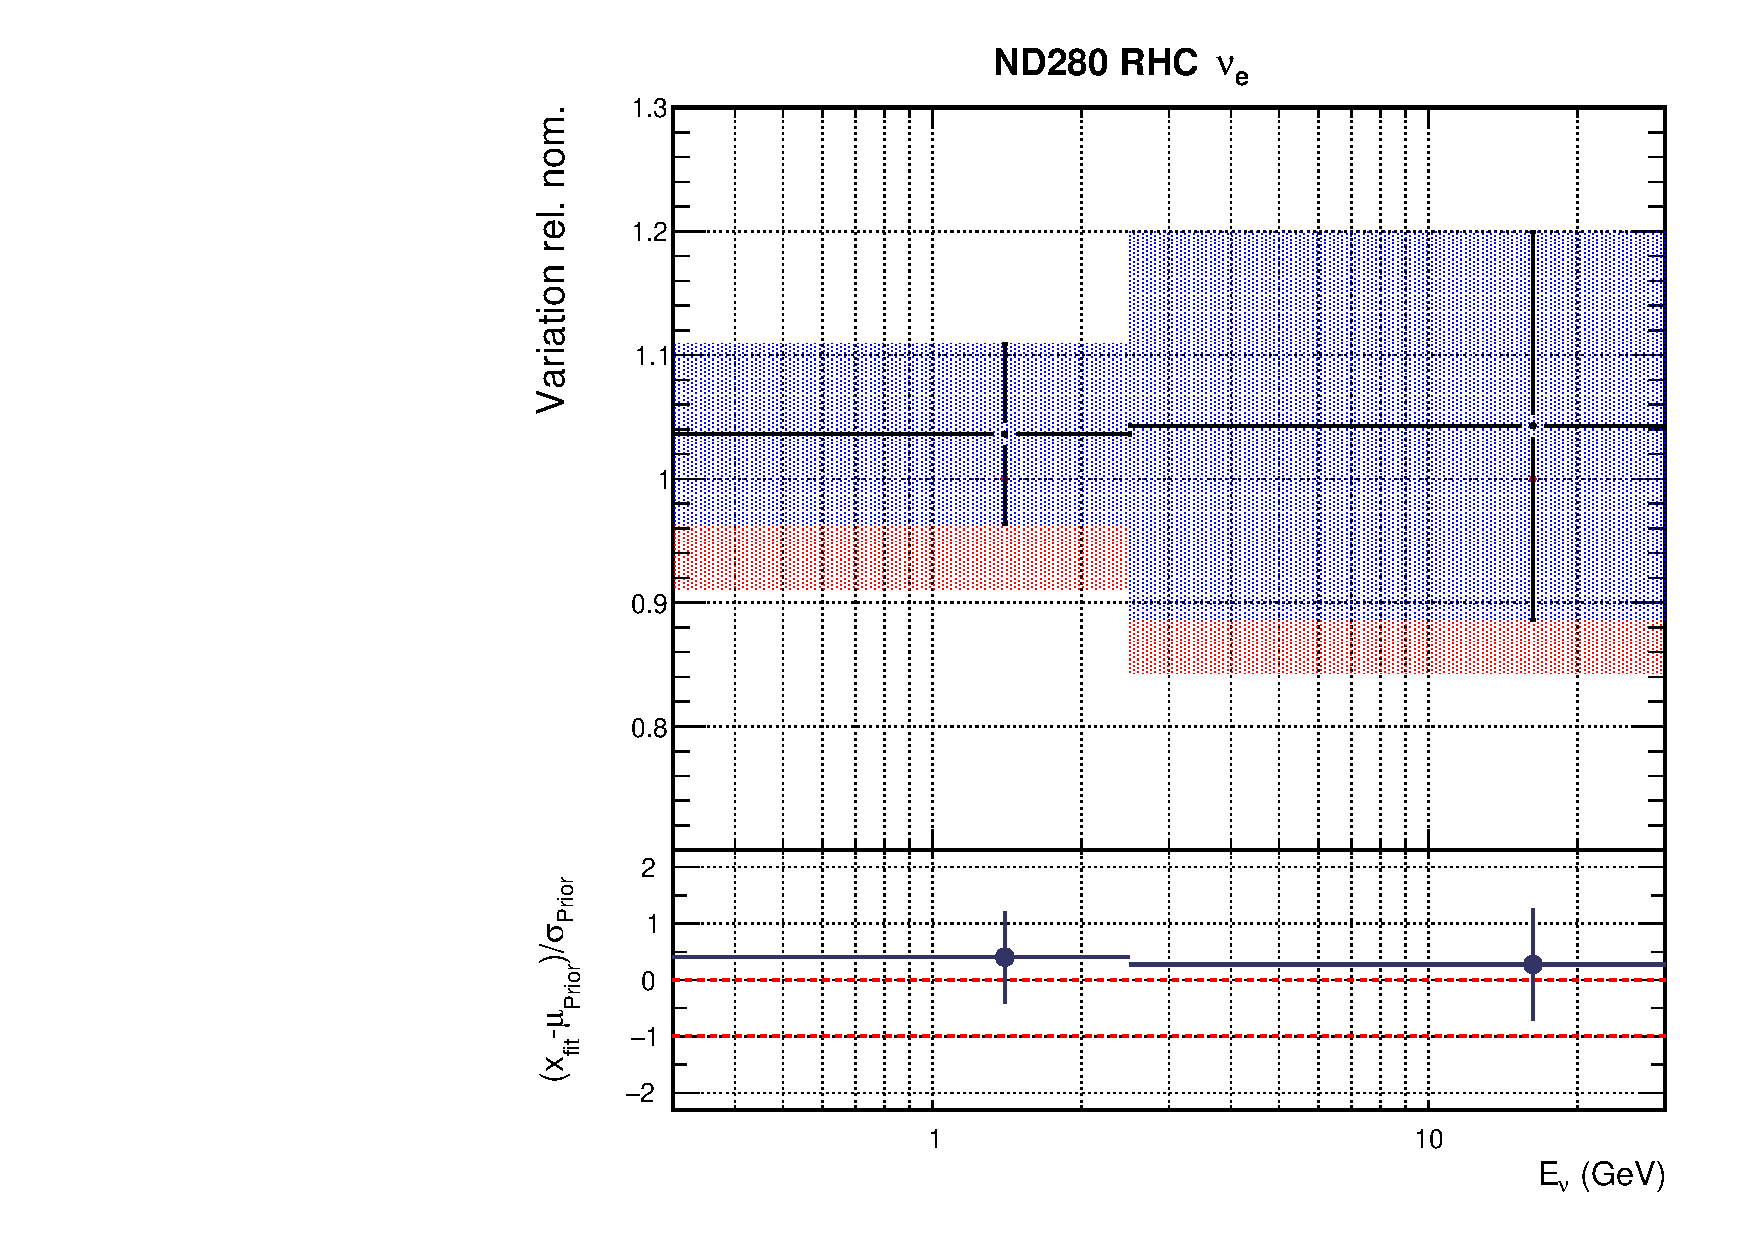
\includegraphics[width=0.95\linewidth]{figs/rhcmpdat248flux_7}
  \caption{ND RHC $\nu_e$}
\end{subfigure}
\begin{subfigure}{0.24\textwidth}
  \centering
  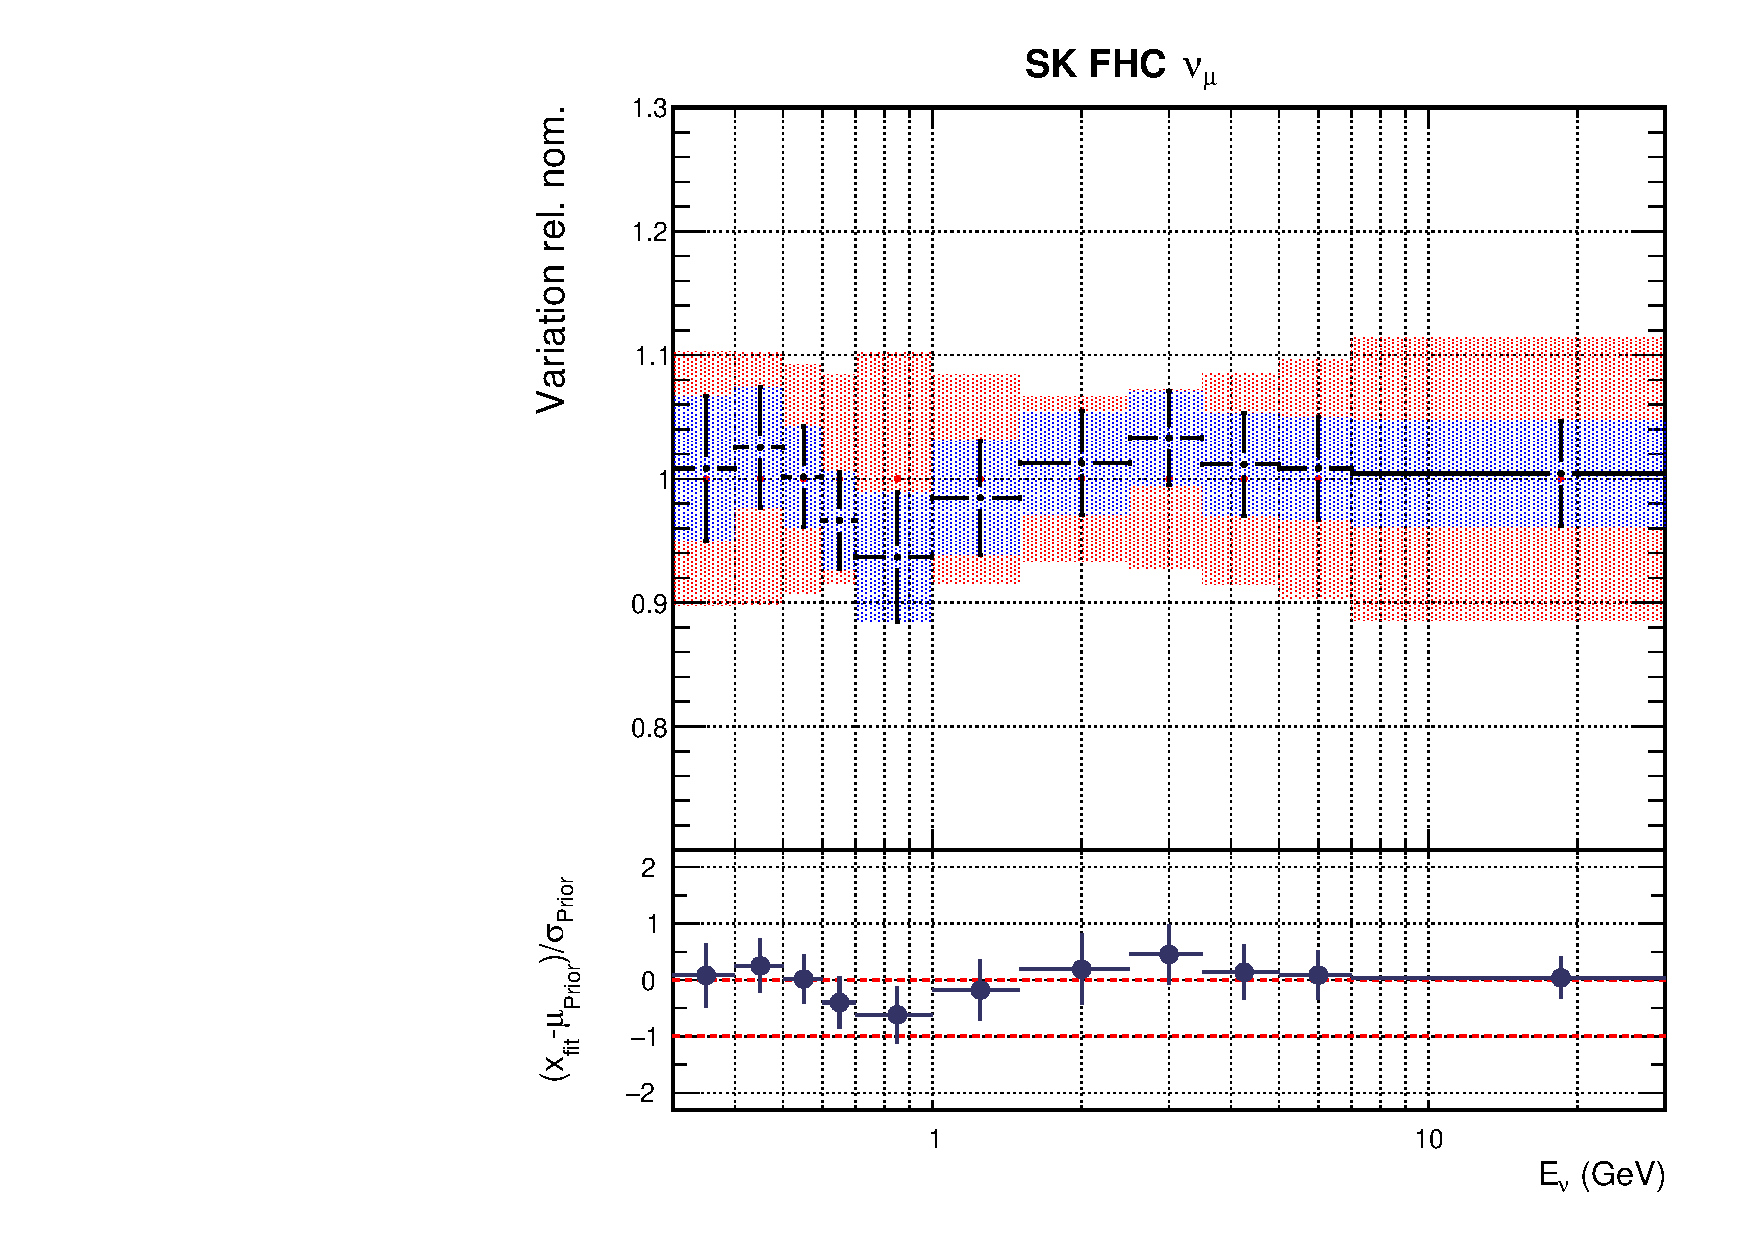
\includegraphics[width=0.95\linewidth]{figs/rhcmpdat248flux_8}
  \caption{SK FHC $\nu_{\mu}$}
\end{subfigure}
\begin{subfigure}{0.24\textwidth}
  \centering
  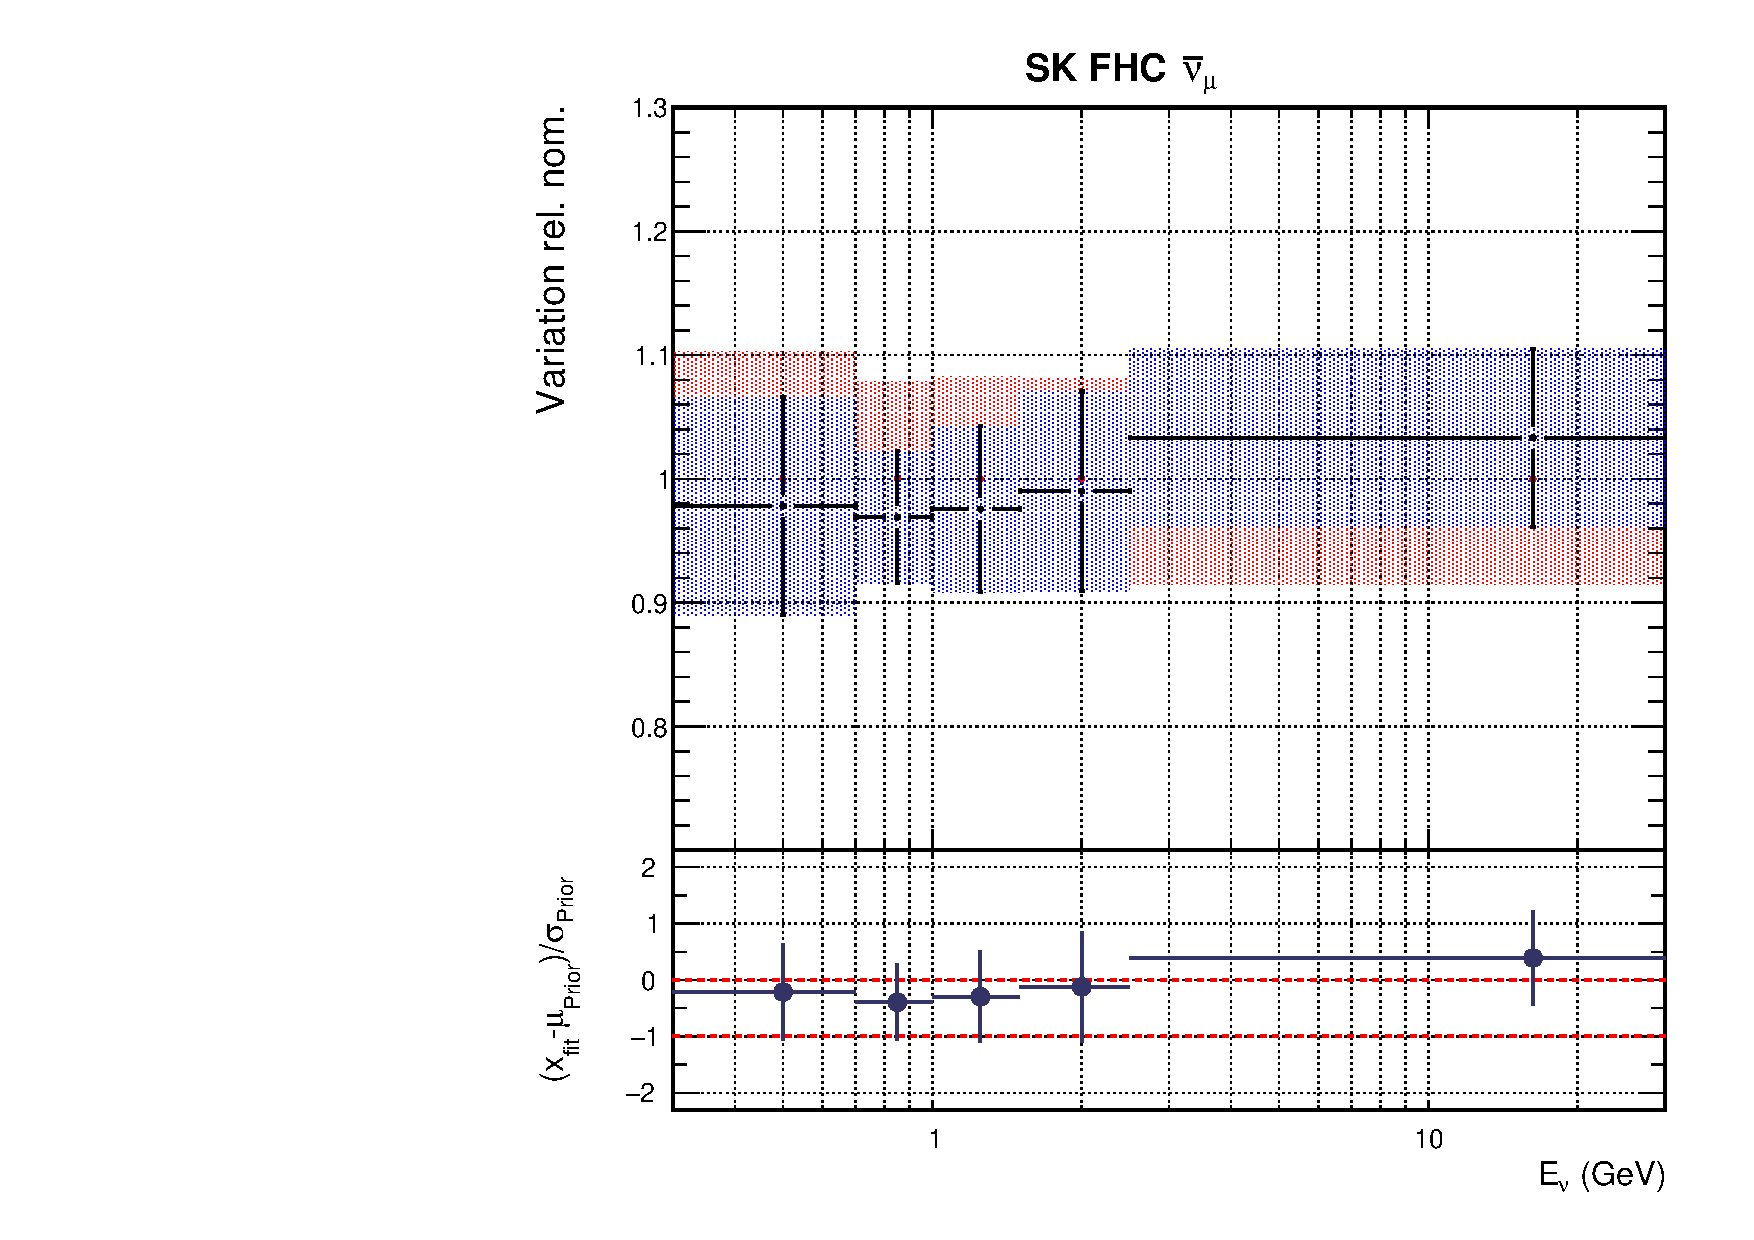
\includegraphics[width=0.95\linewidth]{figs/rhcmpdat248flux_9}
  \caption{SK FHC $\nu_e$}
\end{subfigure}
\begin{subfigure}{0.24\textwidth}
  \centering
  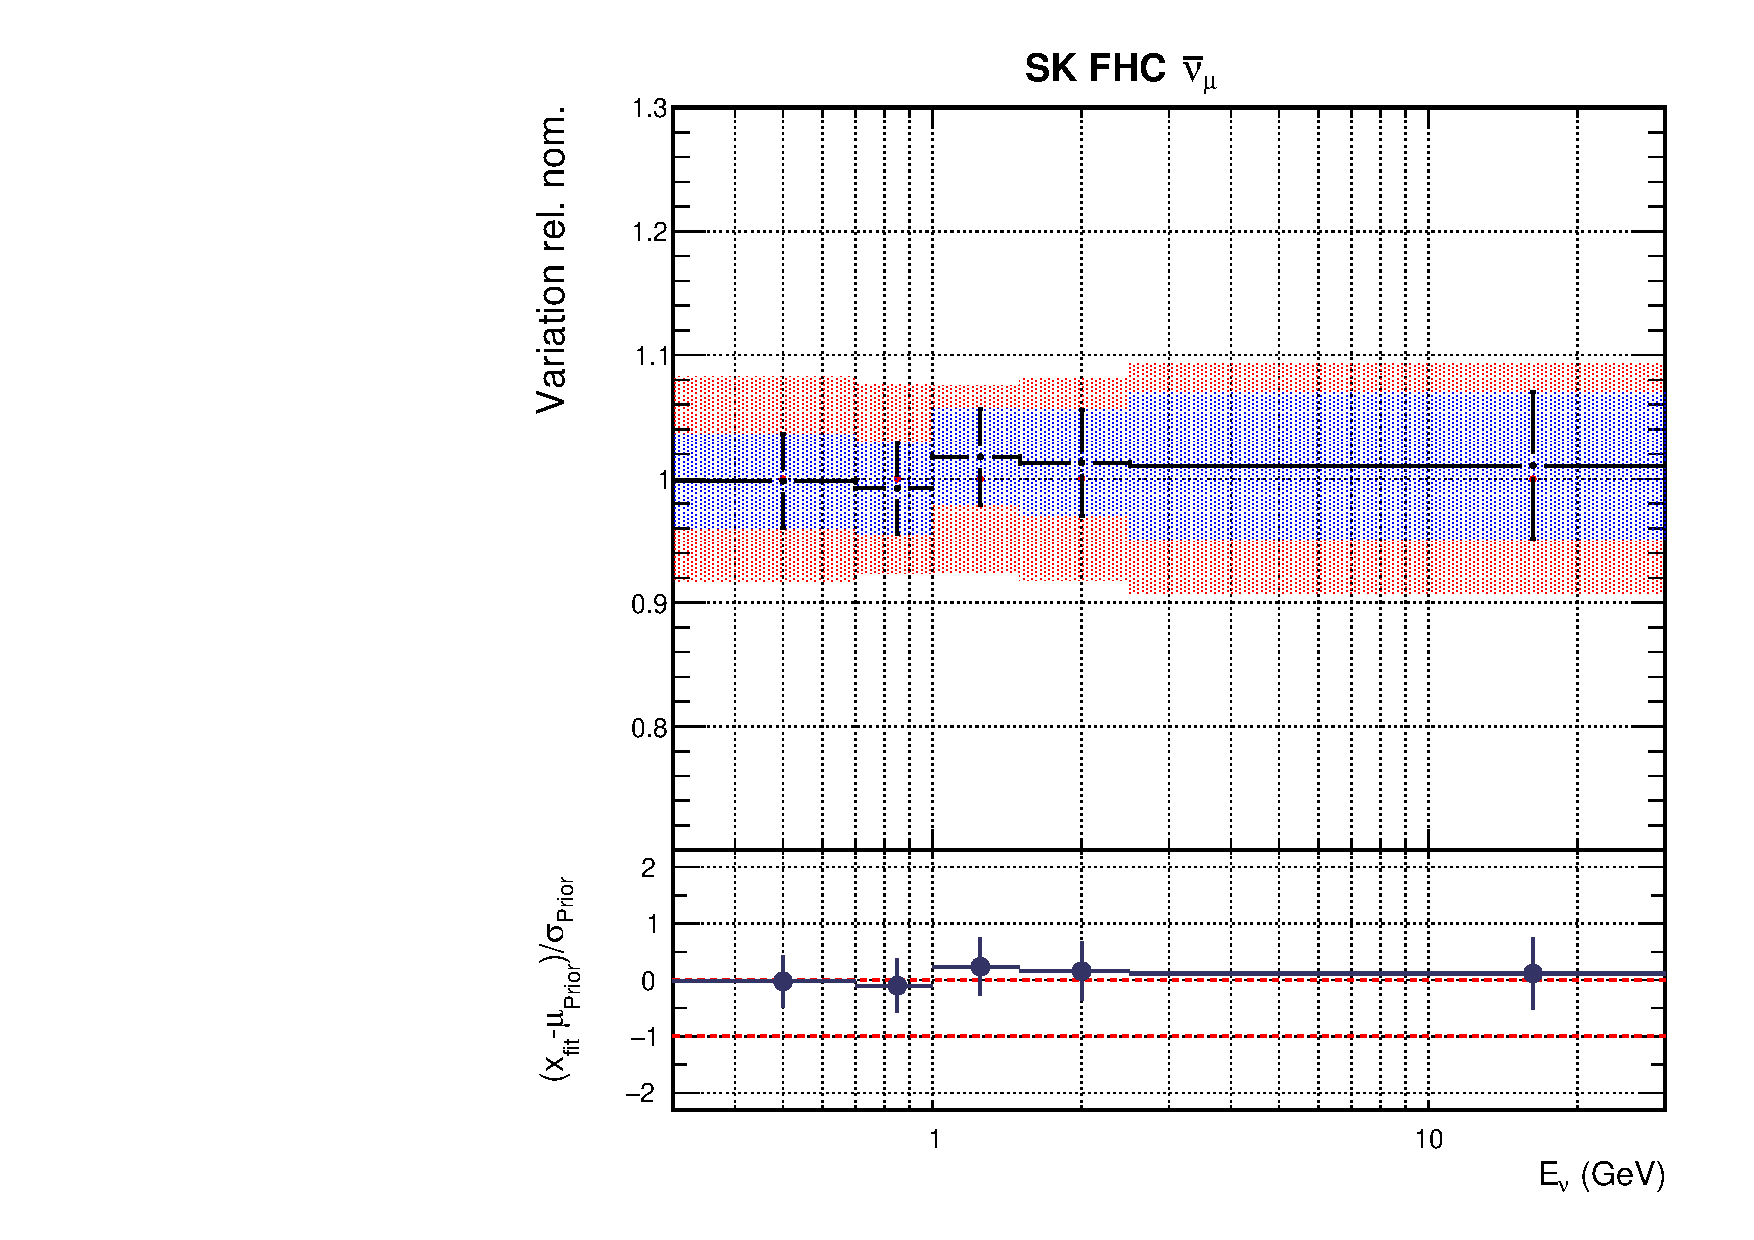
\includegraphics[width=0.95\linewidth]{figs/rhcmpdat248flux_10}
  \caption{SK FHC $\bar{\nu_{\mu}}$}
\end{subfigure}
\begin{subfigure}{0.24\textwidth}
  \centering
  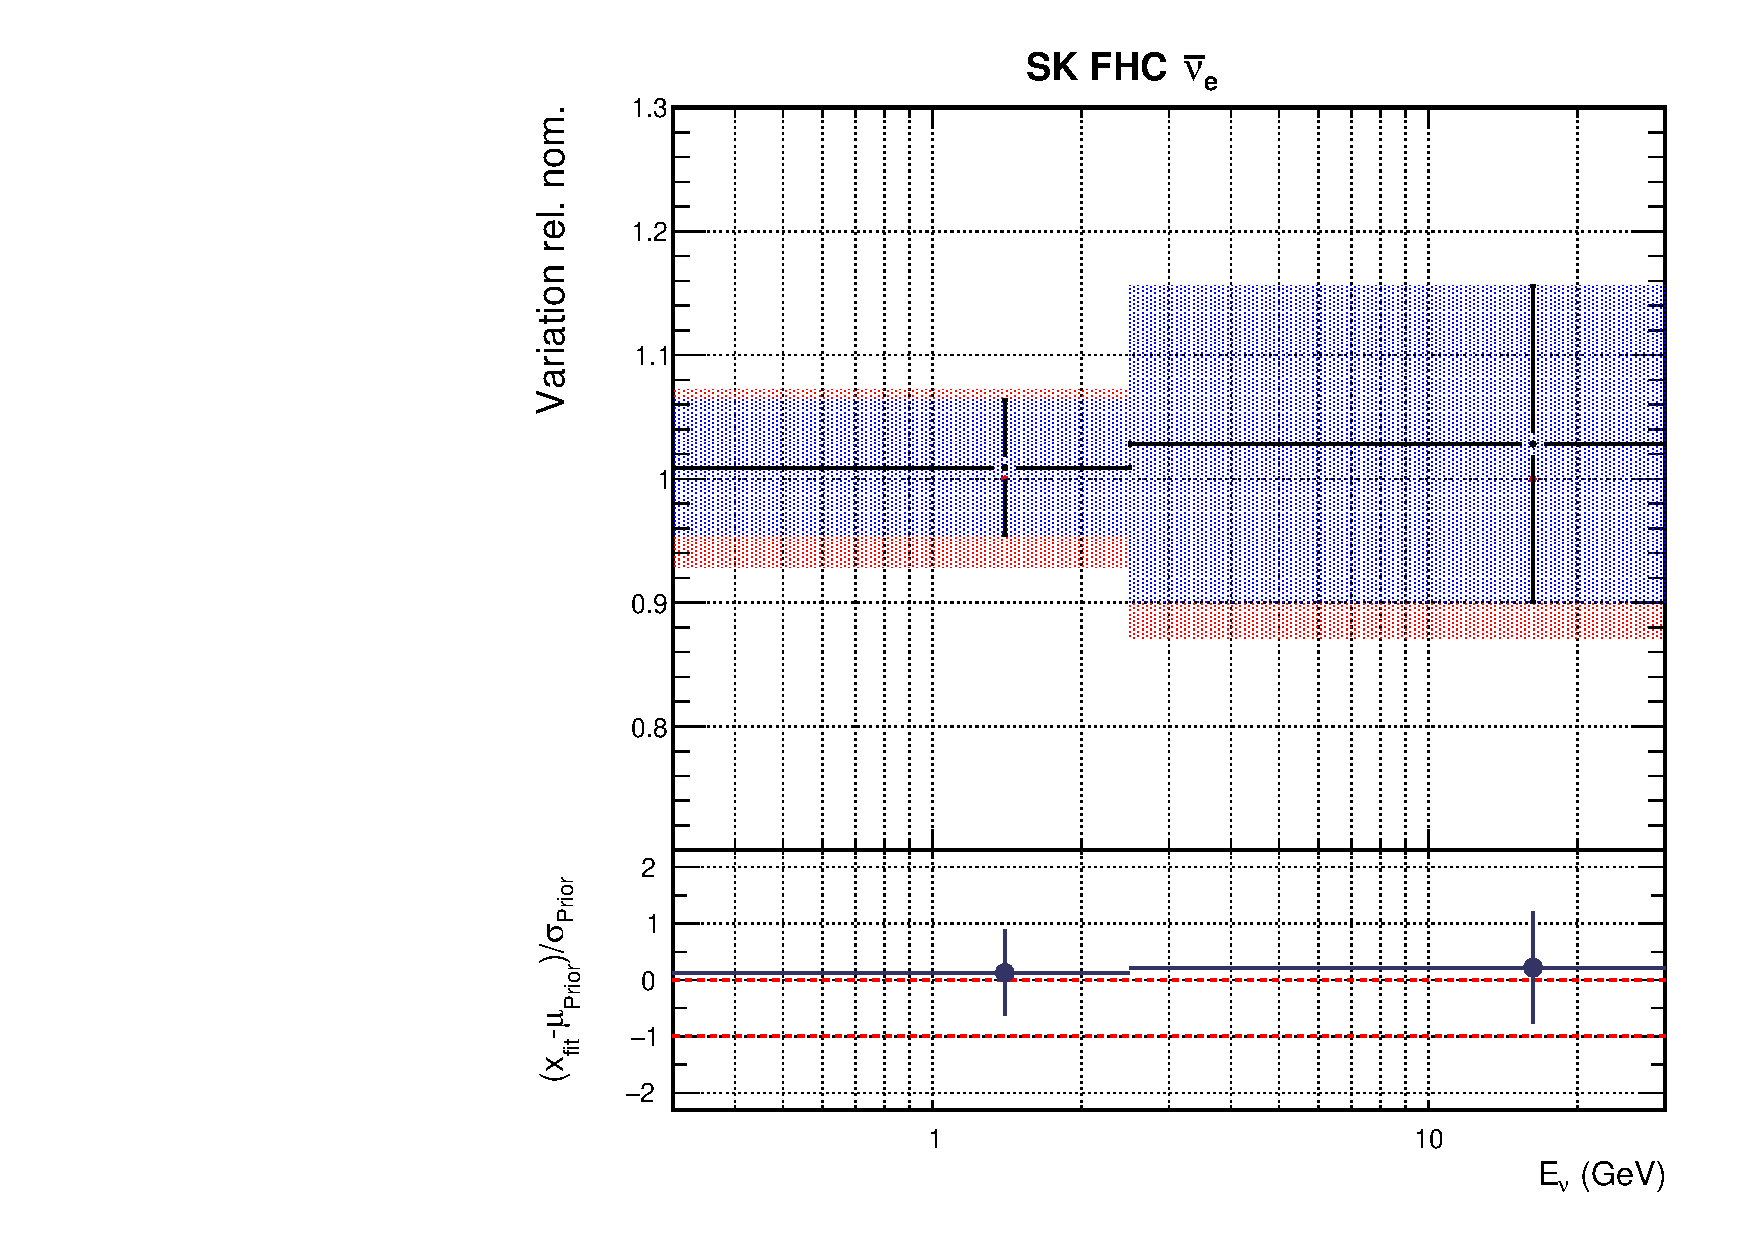
\includegraphics[width=0.95\linewidth]{figs/rhcmpdat248flux_11}
  \caption{SK FHC $\bar{\nu_e}$}
\end{subfigure}
\begin{subfigure}{0.24\textwidth}
  \centering
  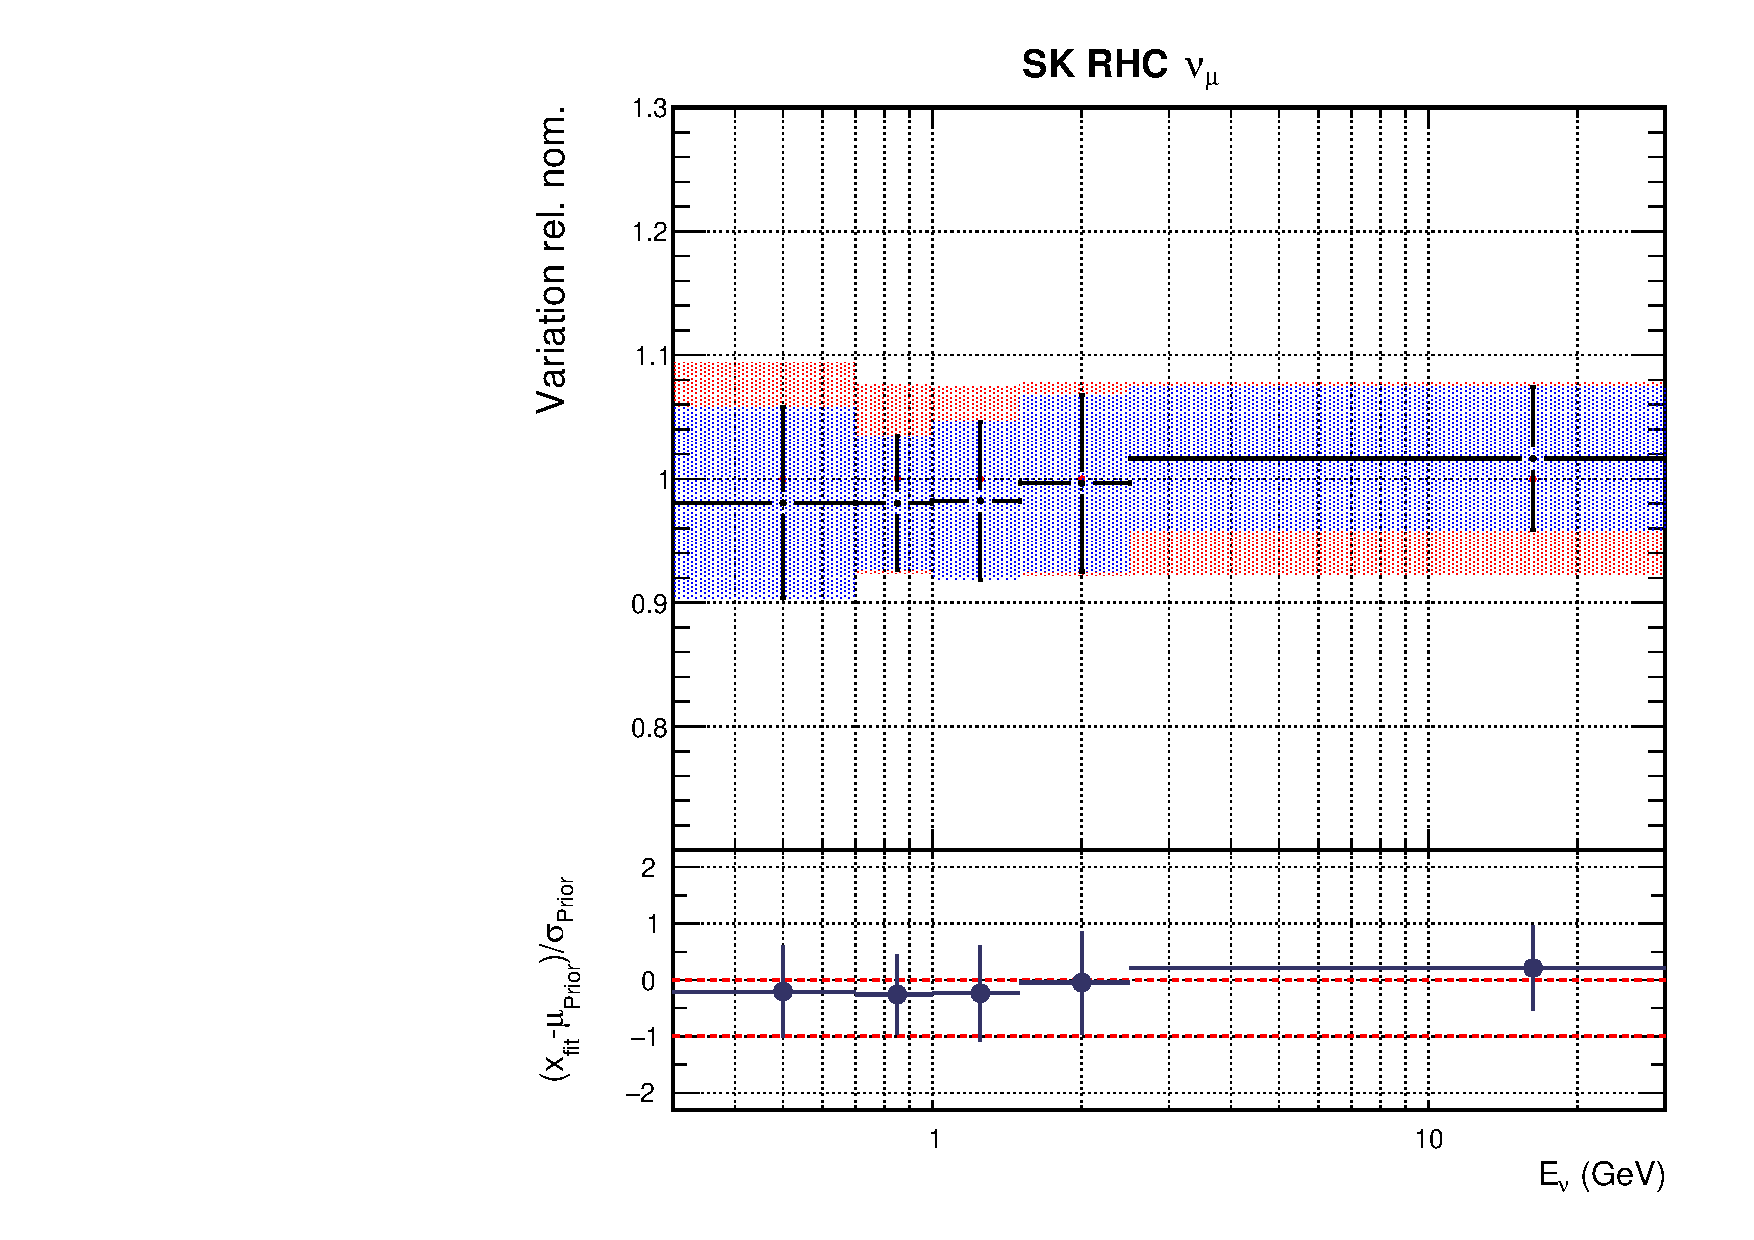
\includegraphics[width=0.95\linewidth]{figs/rhcmpdat248flux_12}
  \caption{SK RHC $\bar{\nu_{\mu}}$}
\end{subfigure}
\begin{subfigure}{0.24\textwidth}
  \centering
  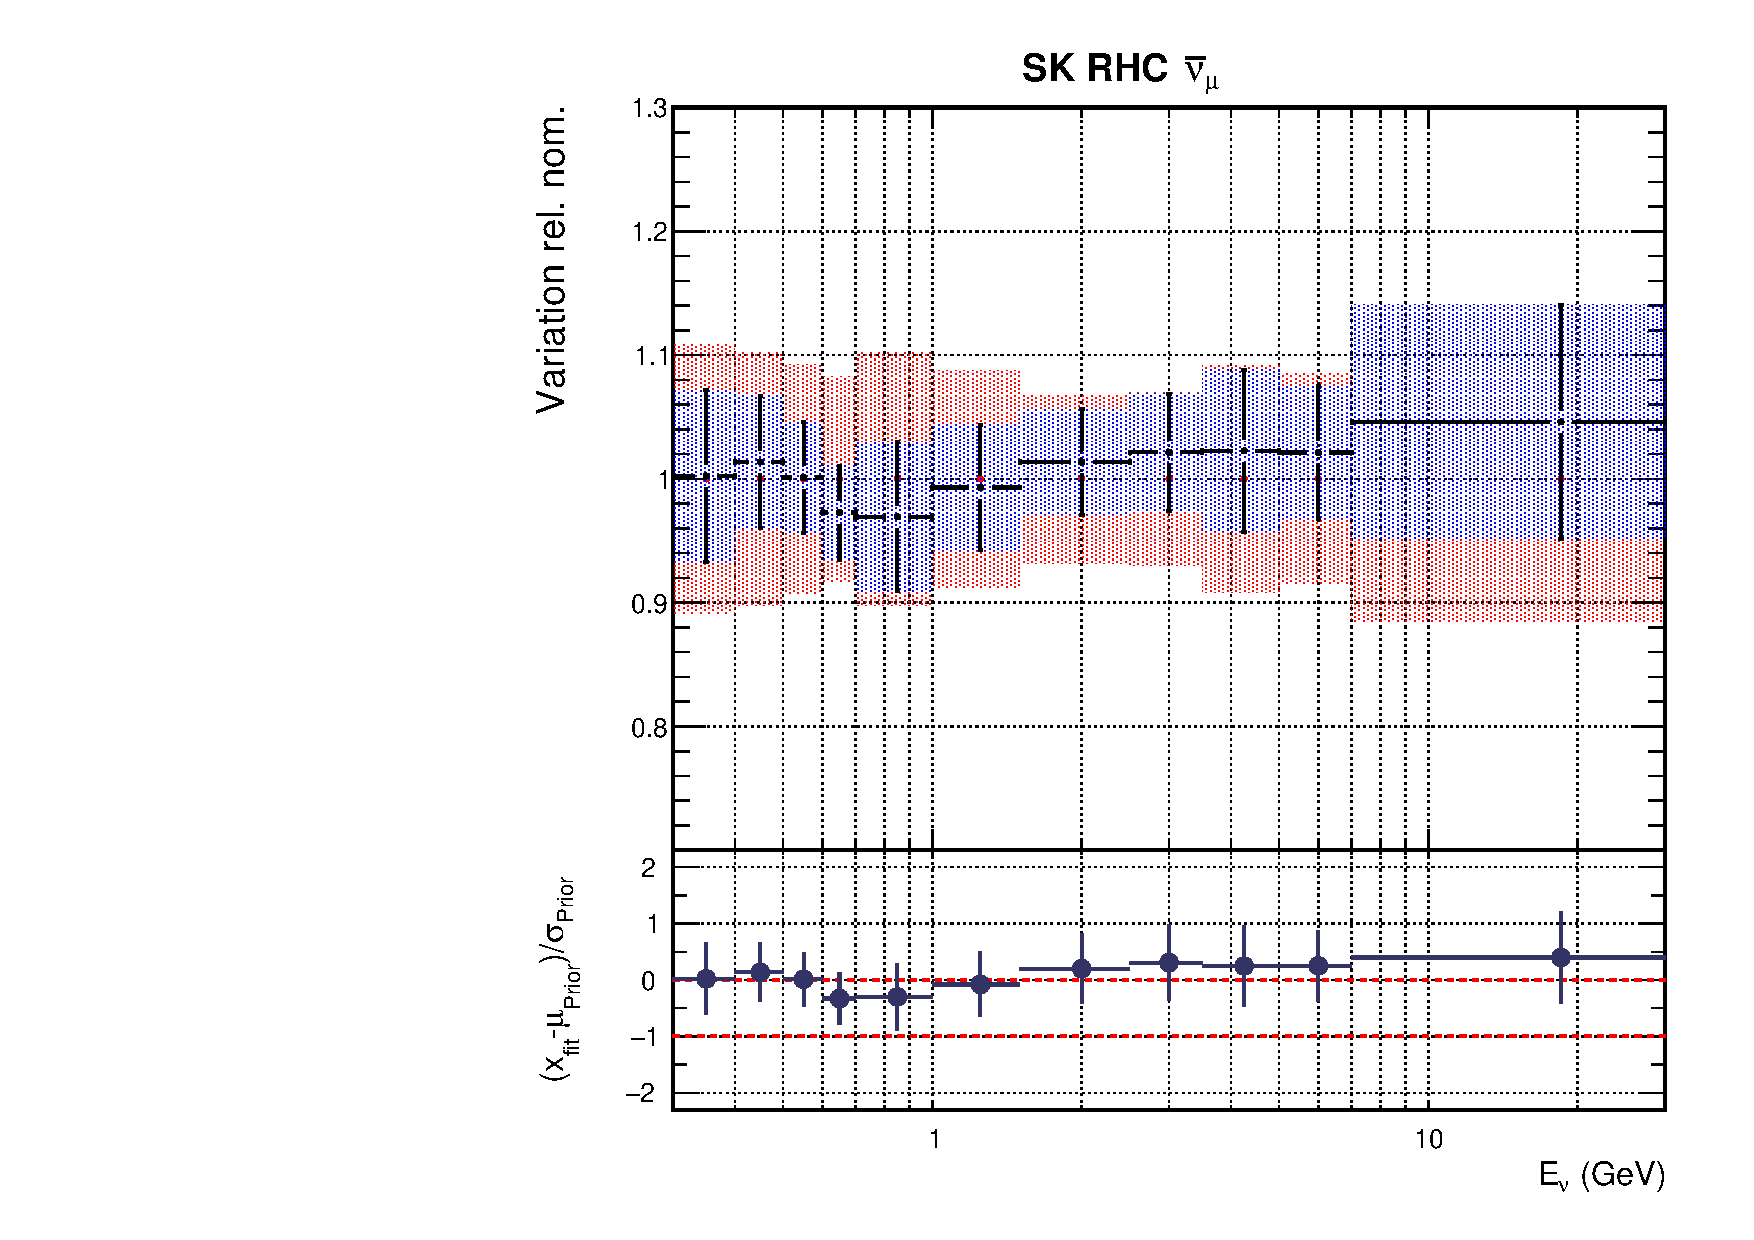
\includegraphics[width=0.95\linewidth]{figs/rhcmpdat248flux_13}
  \caption{SK RHC $\bar{\nu_e}$}
\end{subfigure}
\begin{subfigure}{0.24\textwidth}
  \centering
  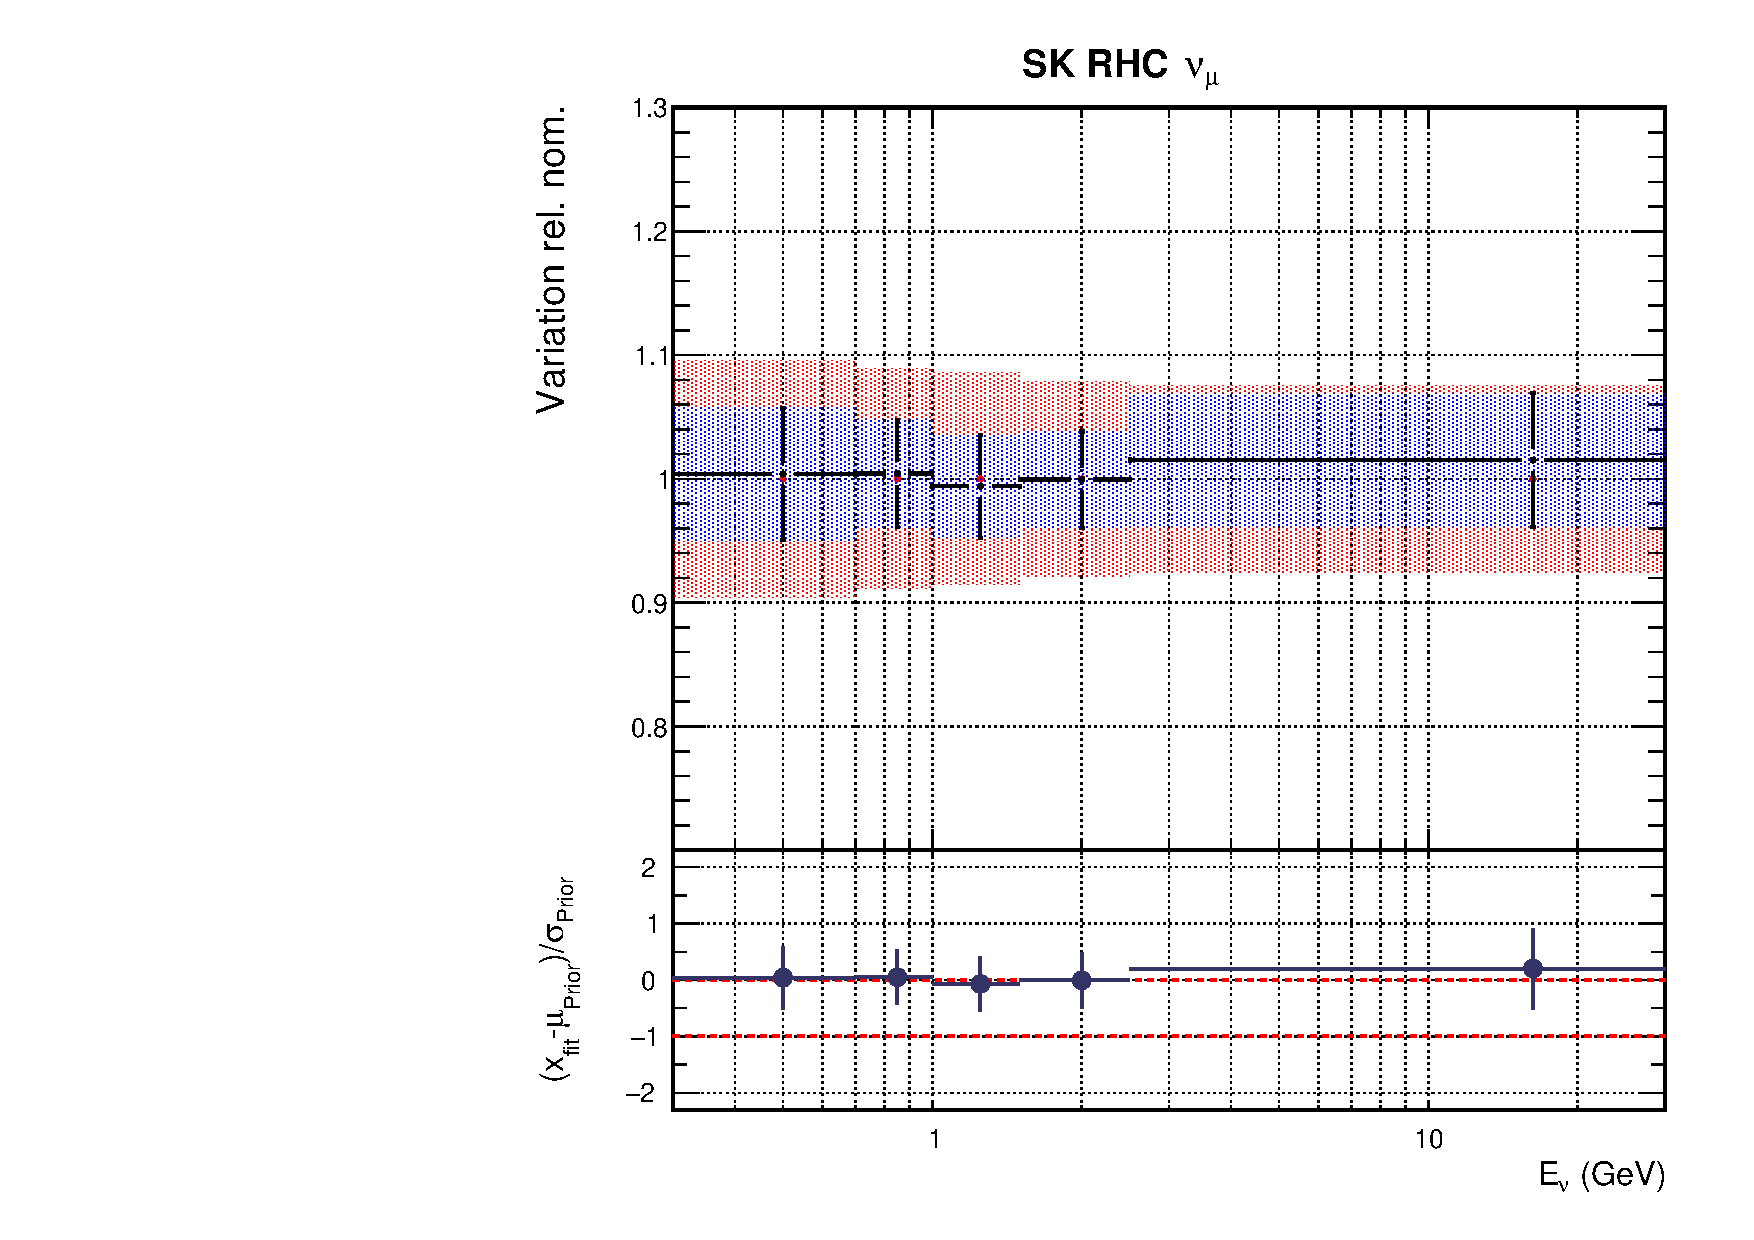
\includegraphics[width=0.95\linewidth]{figs/rhcmpdat248flux_14}
  \caption{SK RHC $\nu_{\mu}$}
\end{subfigure}
\begin{subfigure}{0.24\textwidth}
  \centering
  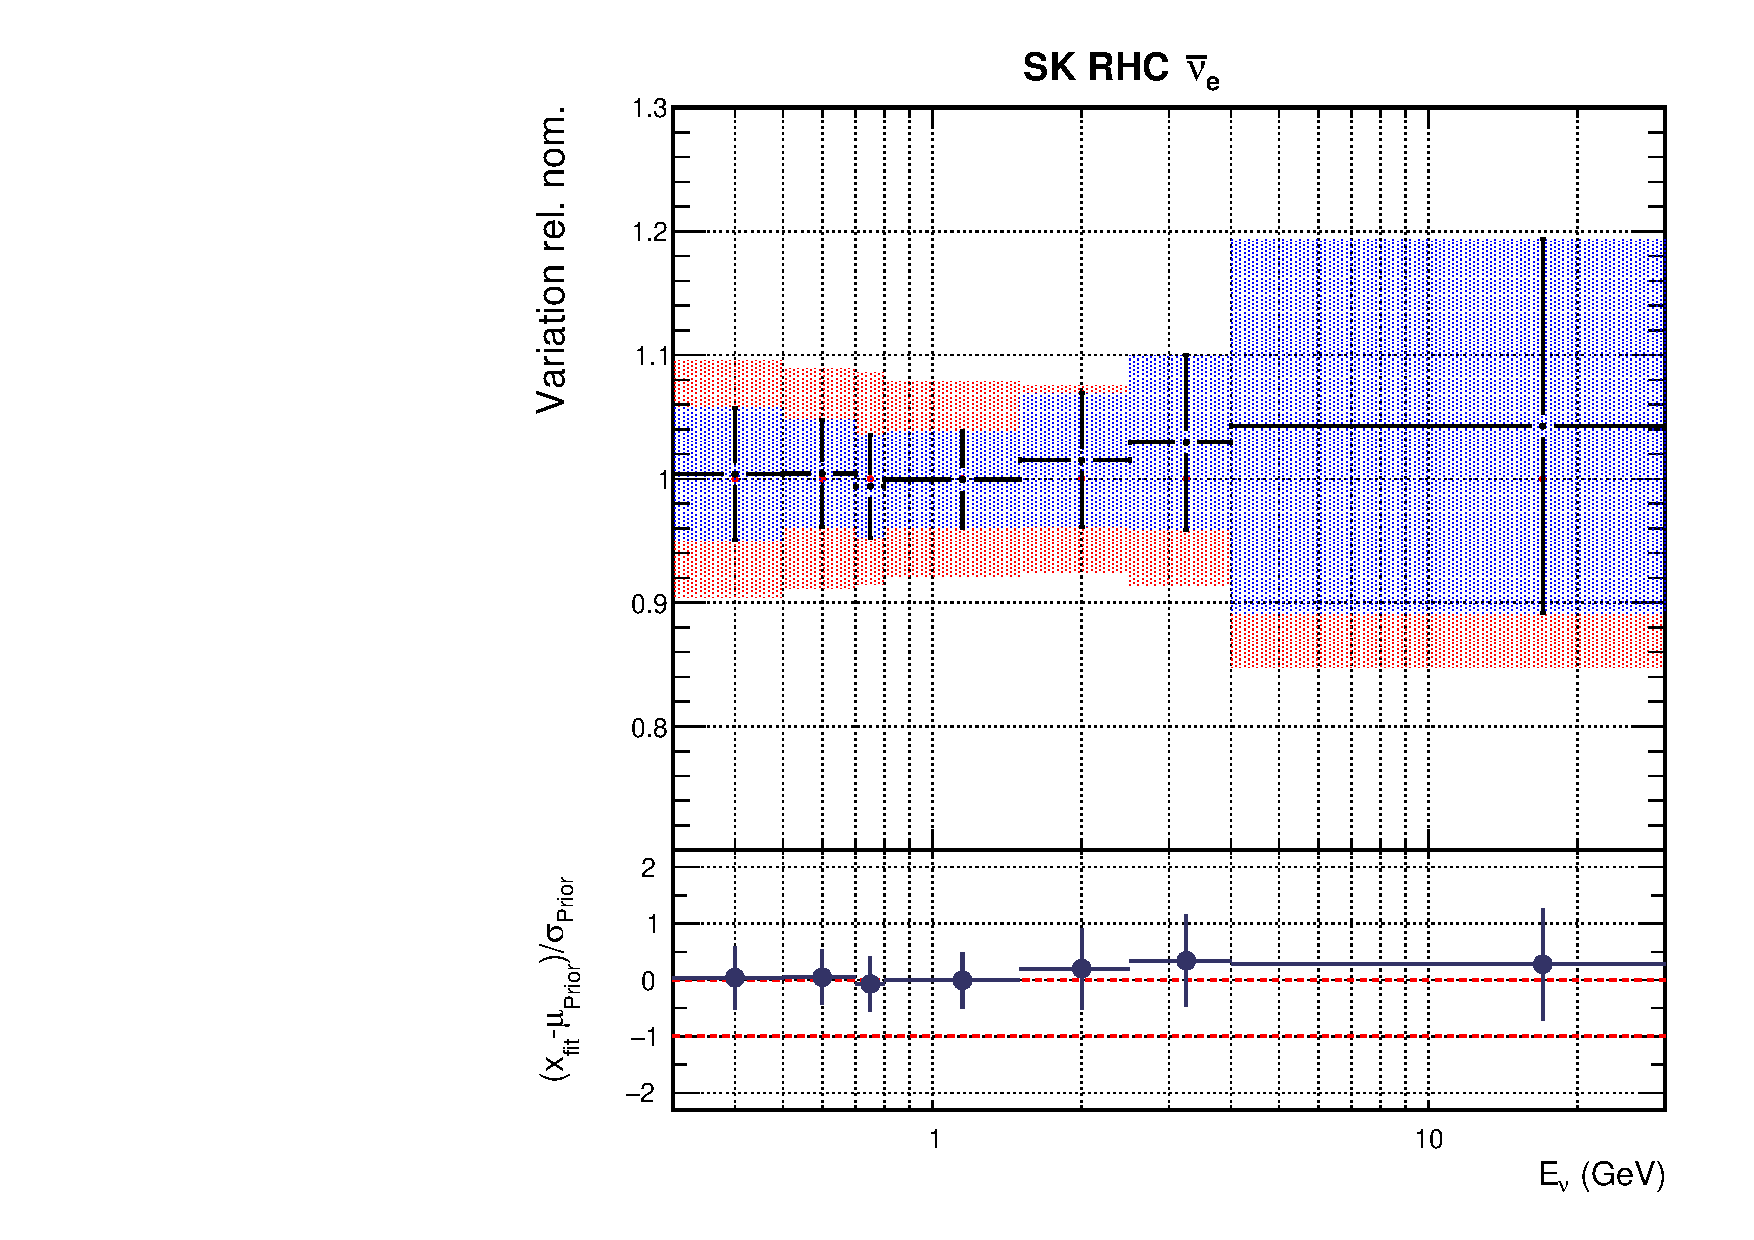
\includegraphics[width=0.95\linewidth]{figs/rhcmpdat248flux_15}
  \caption{SK RHC $\nu_e$}
\end{subfigure}
\caption{Flux parameters for Asimov fits using FHC only data}
\label{fig:rhcmpidat248fluxSK}
\end{figure}

\begin{figure}
\centering
\begin{subfigure}{0.95\textwidth}
  \centering
  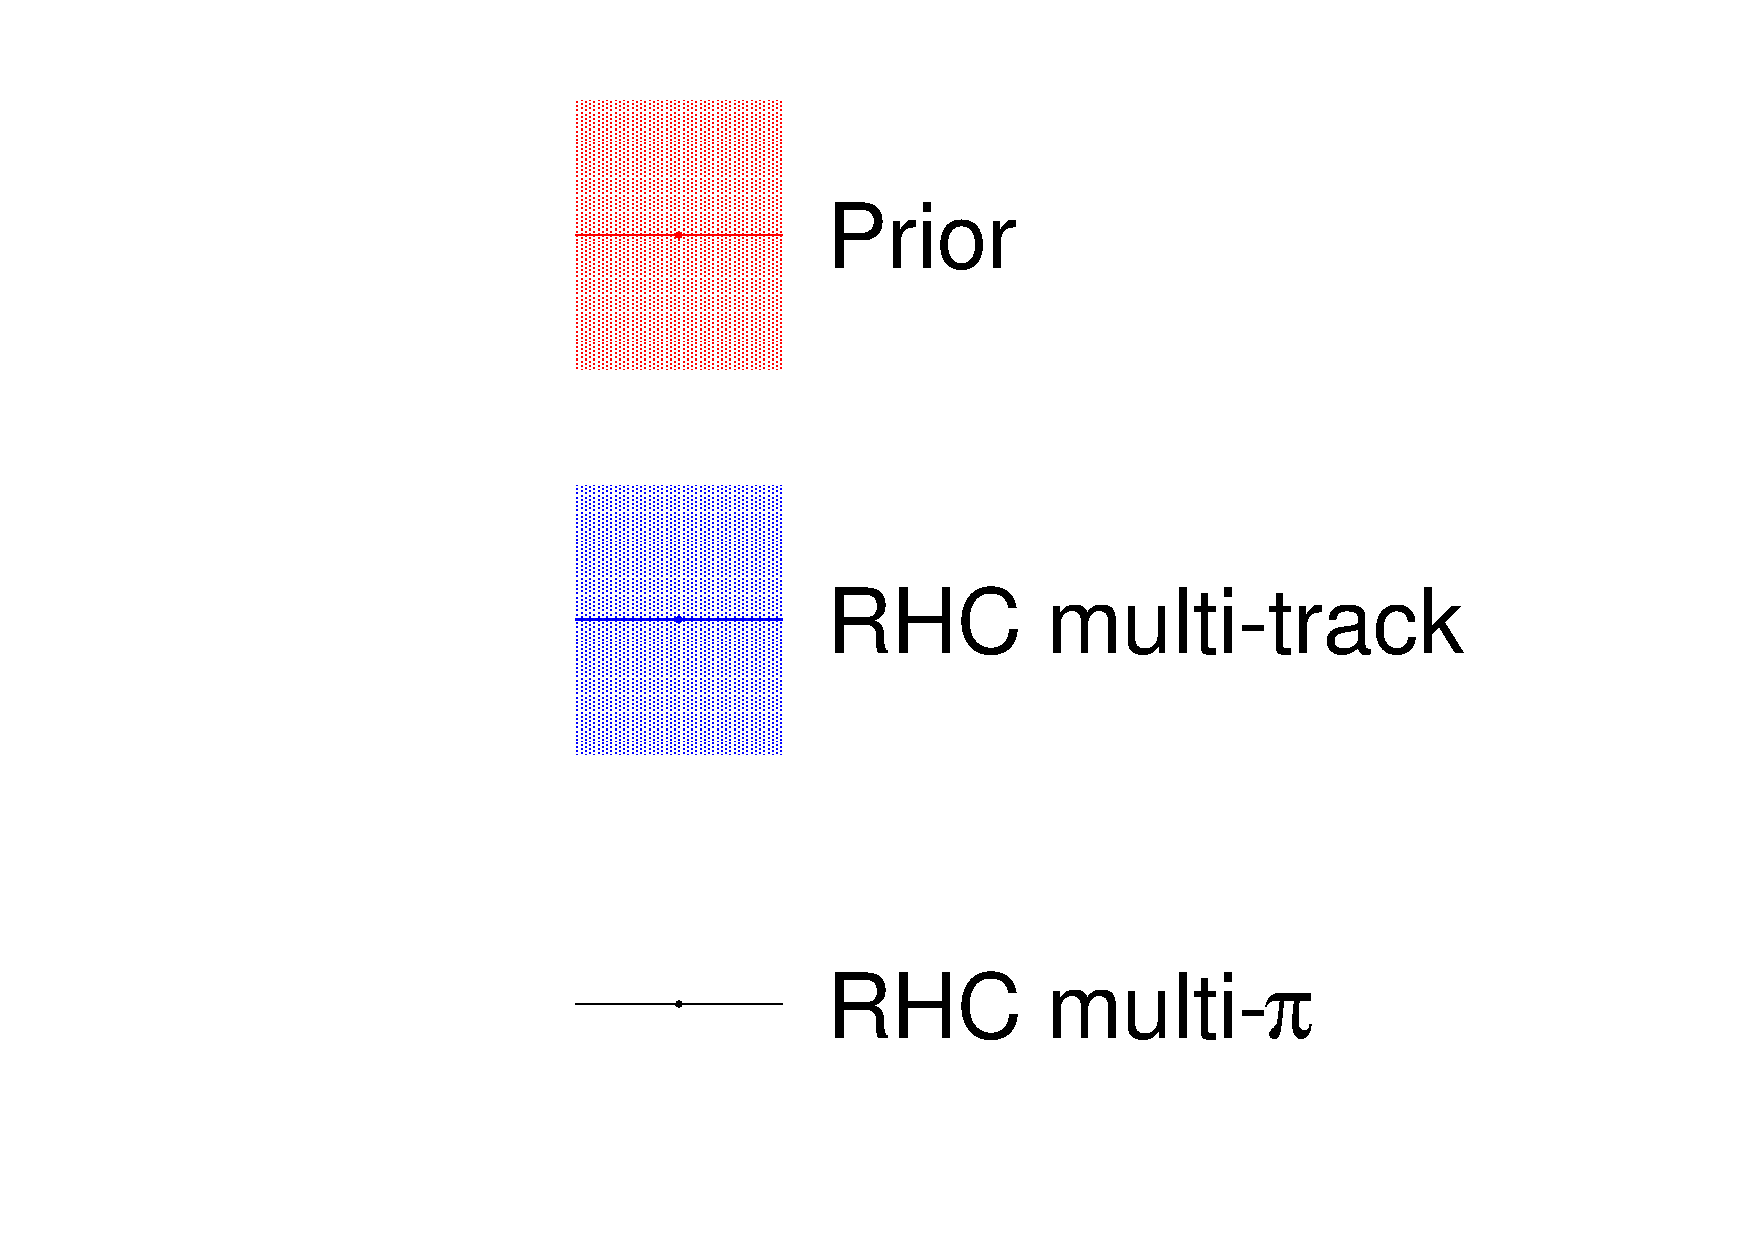
\includegraphics[width=0.25\linewidth]{figs/rhcmpdat248_leg}	
\end{subfigure}
\begin{subfigure}{0.49\textwidth}
  \centering
  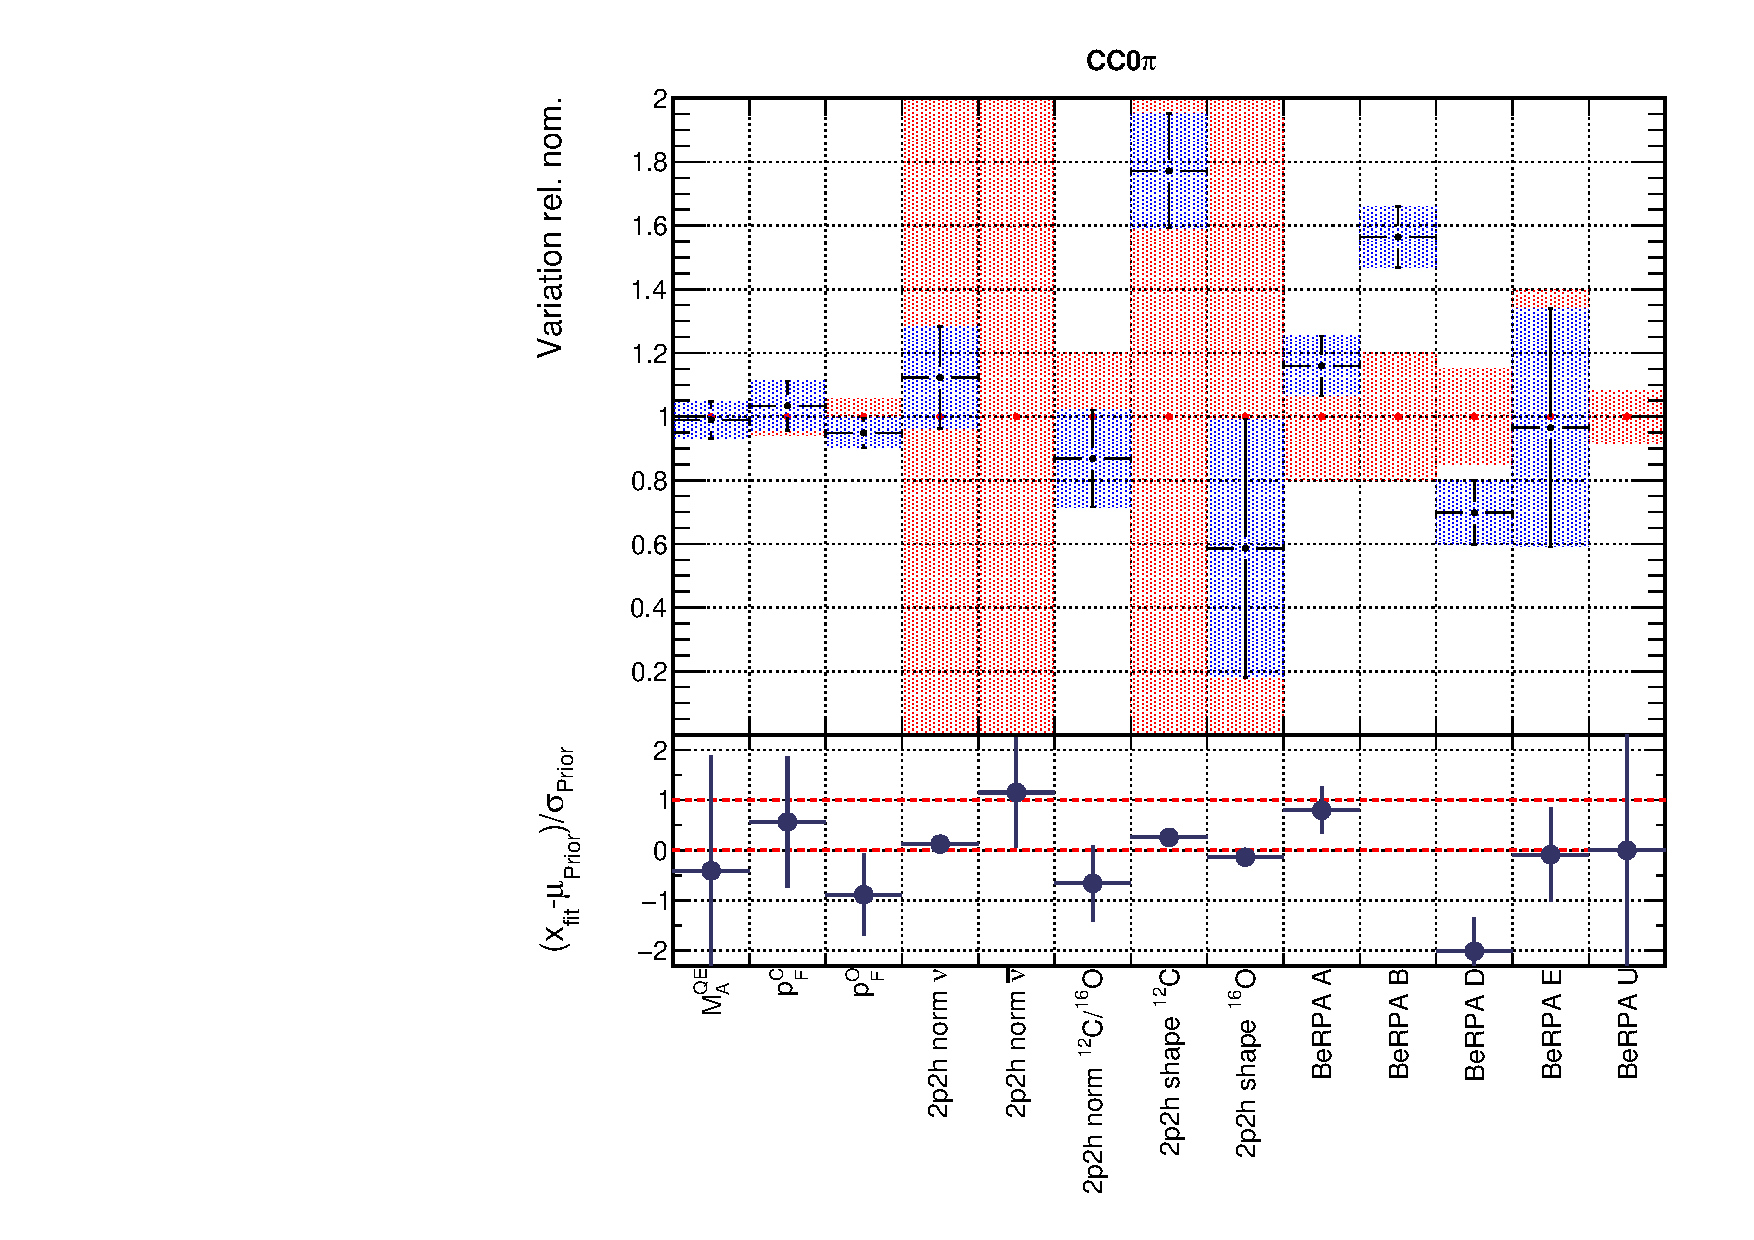
\includegraphics[width=0.95\linewidth]{figs/rhcmpdatxsec248_1}
  \caption{CC0$\pi$}
\end{subfigure}
\begin{subfigure}{0.49\textwidth}
  \centering
  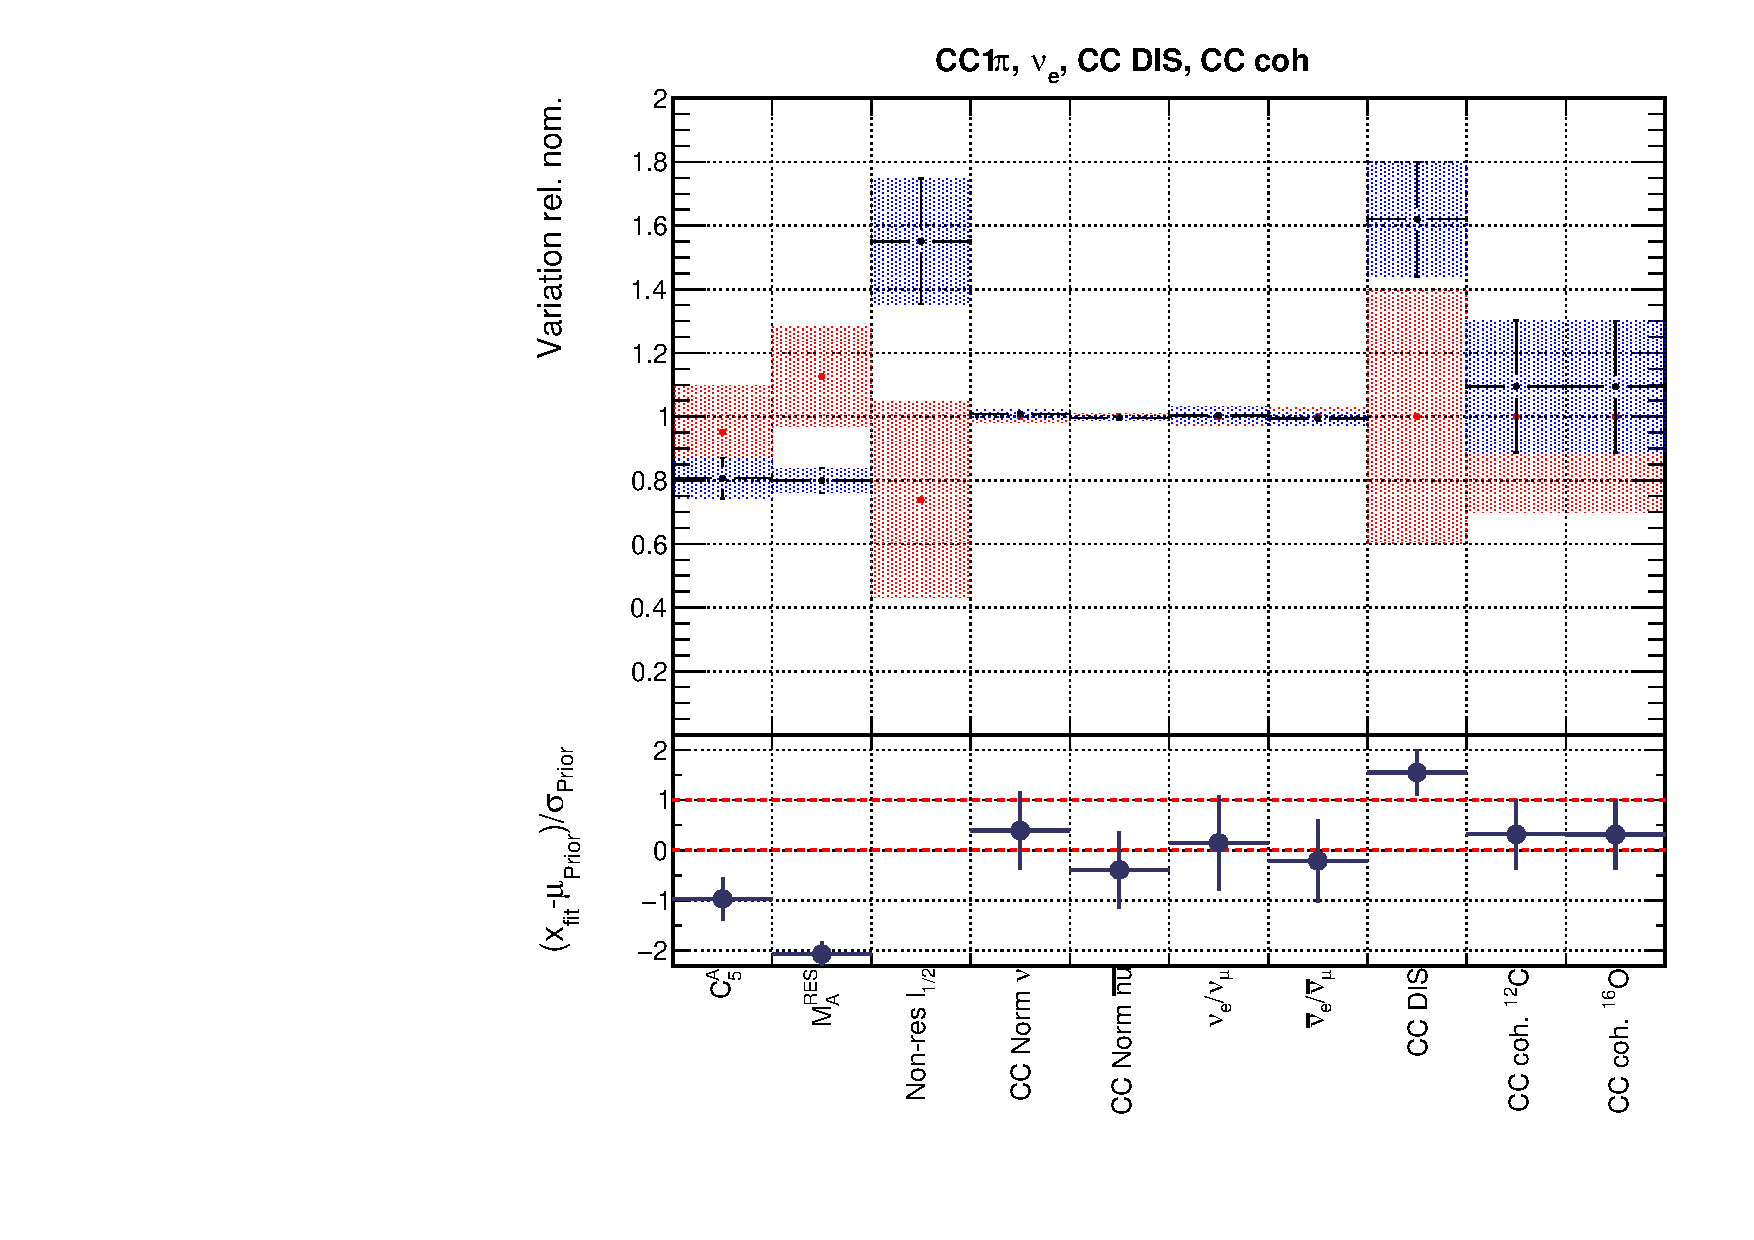
\includegraphics[width=0.95\linewidth]{figs/rhcmpdatxsec248_2}
  \caption{CC1$\pi$, $\nu_e$, CC DIS, and CC coh.}
\end{subfigure}
\begin{subfigure}{0.49\textwidth}
  \centering
  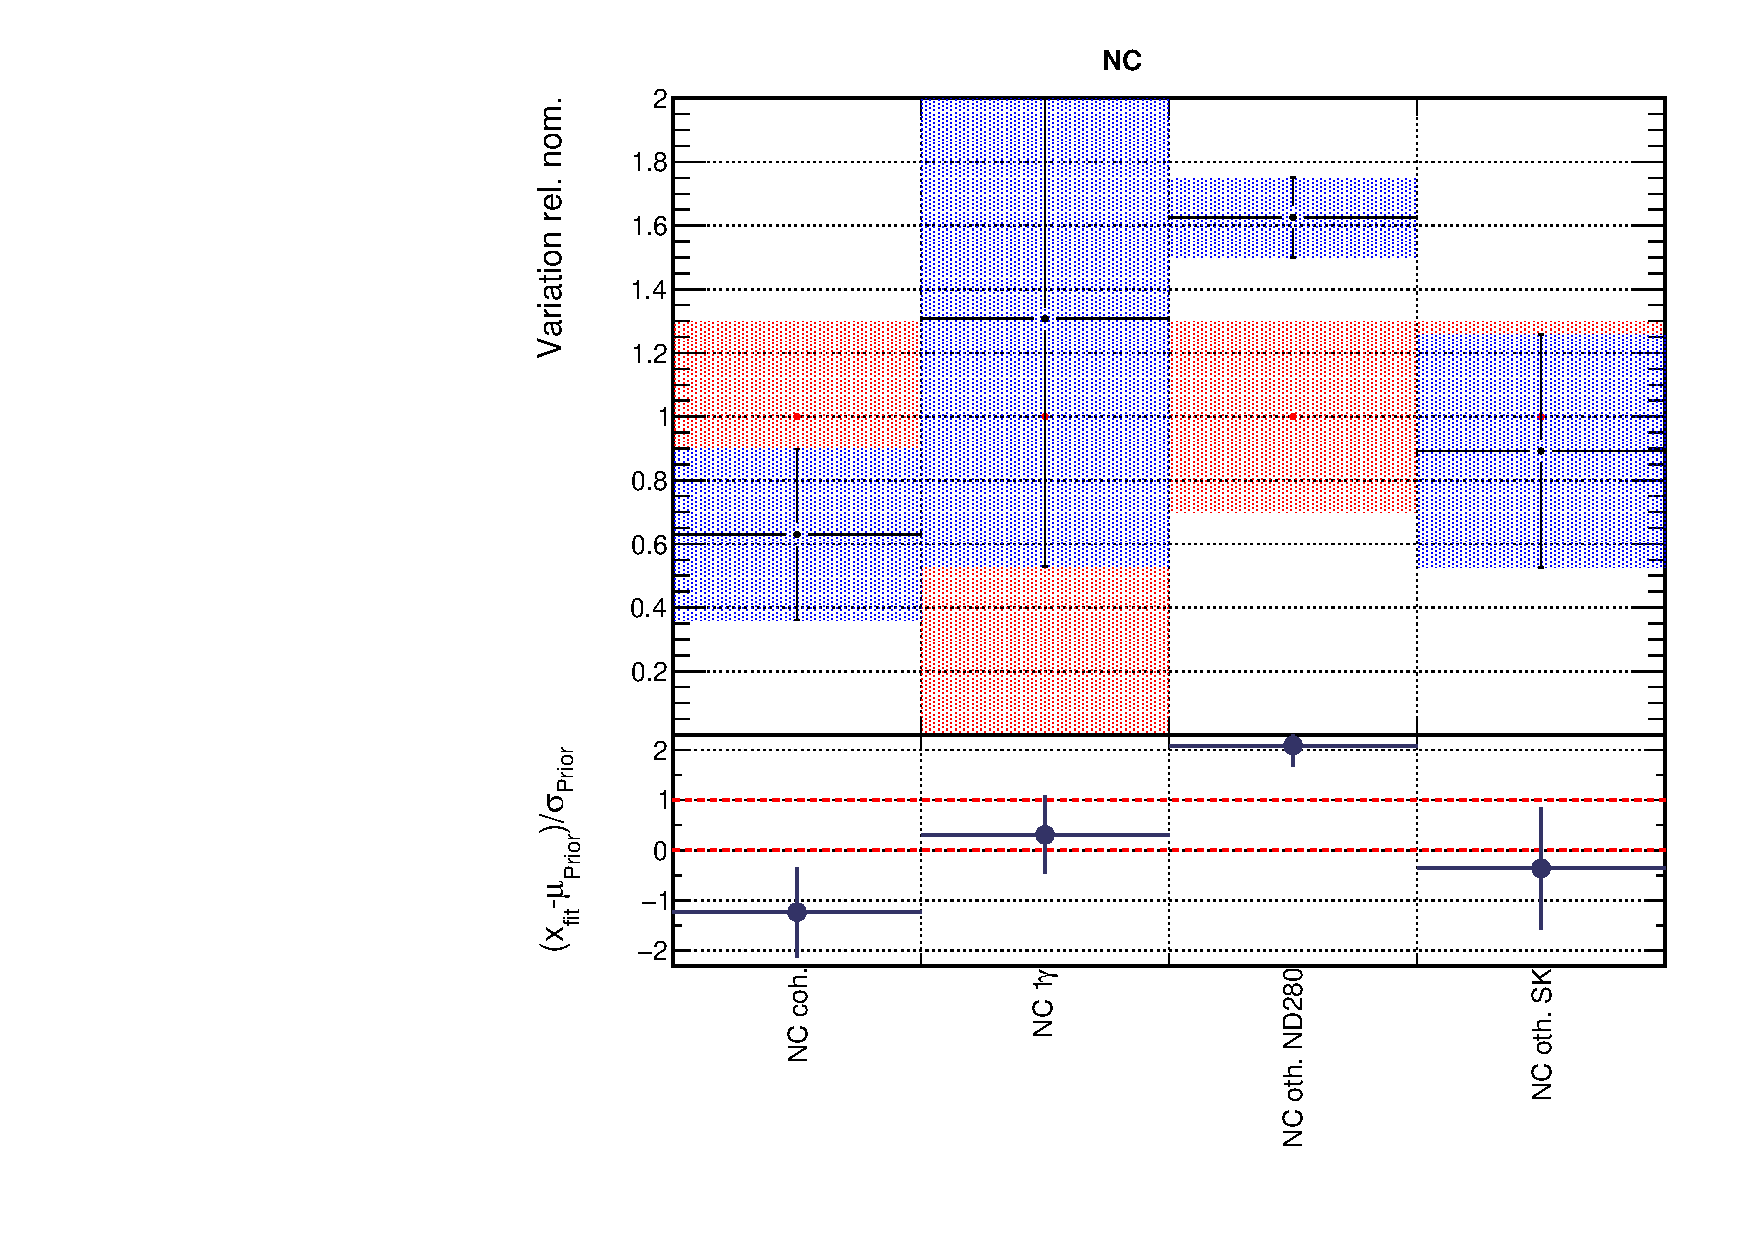
\includegraphics[width=0.95\linewidth]{figs/rhcmpdatxsec248_3}
  \caption{NC}
\end{subfigure}
\begin{subfigure}{0.49\textwidth}
  \centering
  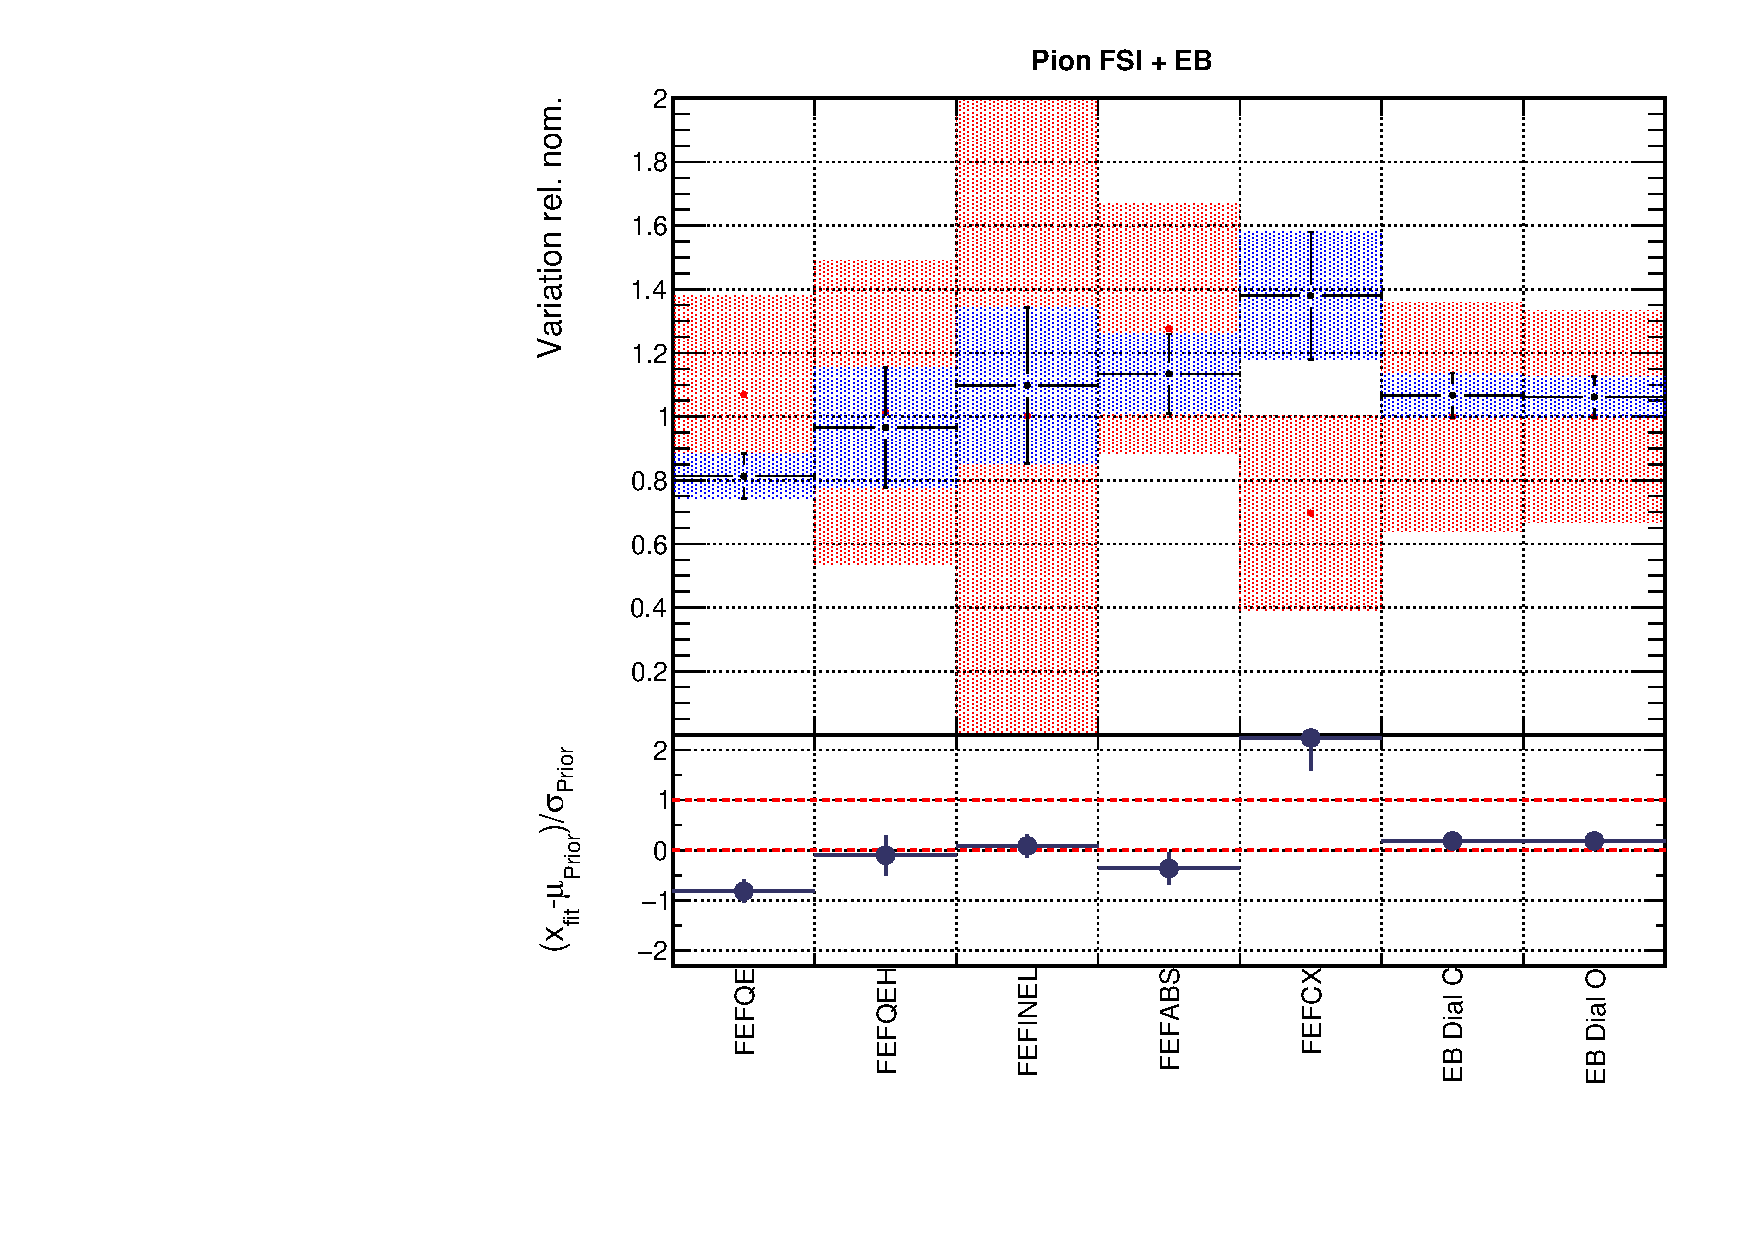
\includegraphics[width=0.95\linewidth]{figs/rhcmpdatxsec248_4}
  \caption{$\pi$ FSI and $E_b$}
\end{subfigure}
\caption{Interaction parameters for data fits using FHC only data.}
\label{fig:rhcmpidat248xsec}
\end{figure}

To see the full impact of the change in samples, Asimov and data fits were run with the multi-$\pi$ and track implementations, using FHC and RHC data (runs 2-8). The Asimov fit results, shown in Figures \ref{fig:rhcmpiasmvSK} and \ref{fig:rhcmpiasmvxsec}, are very similar for the two samples. The slight differences are due to marginalisation effects, and the two fits are entirely compatible. There is a very slight reduction in uncertainties using the RHC multi-$\pi$ samples, showing a small improvement in sensitivity.

\begin{figure}[t]
\centering
\begin{subfigure}{0.95\textwidth}
  \centering
  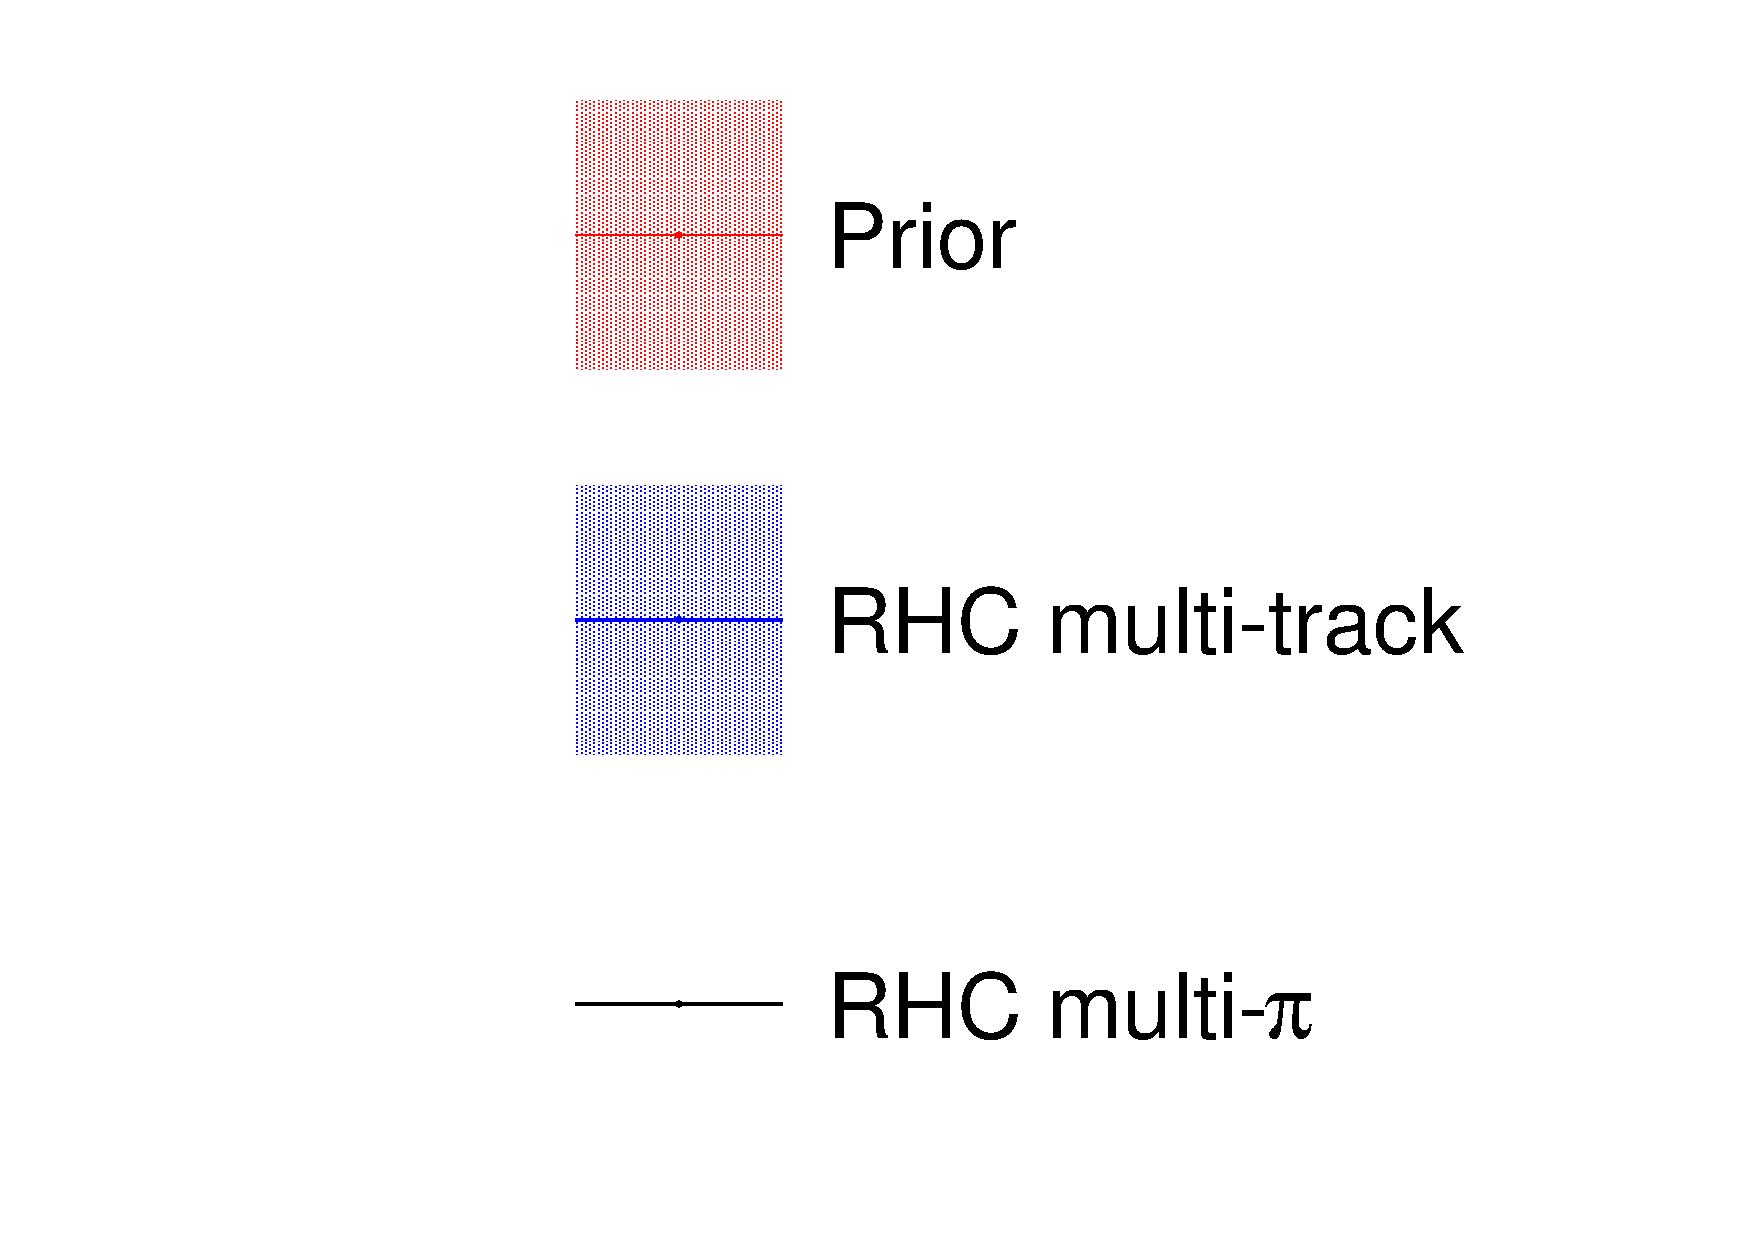
\includegraphics[width=0.24\linewidth]{figs/rhcmpasmv_leg}	
\end{subfigure}
\begin{subfigure}{0.24\textwidth}
  \centering
  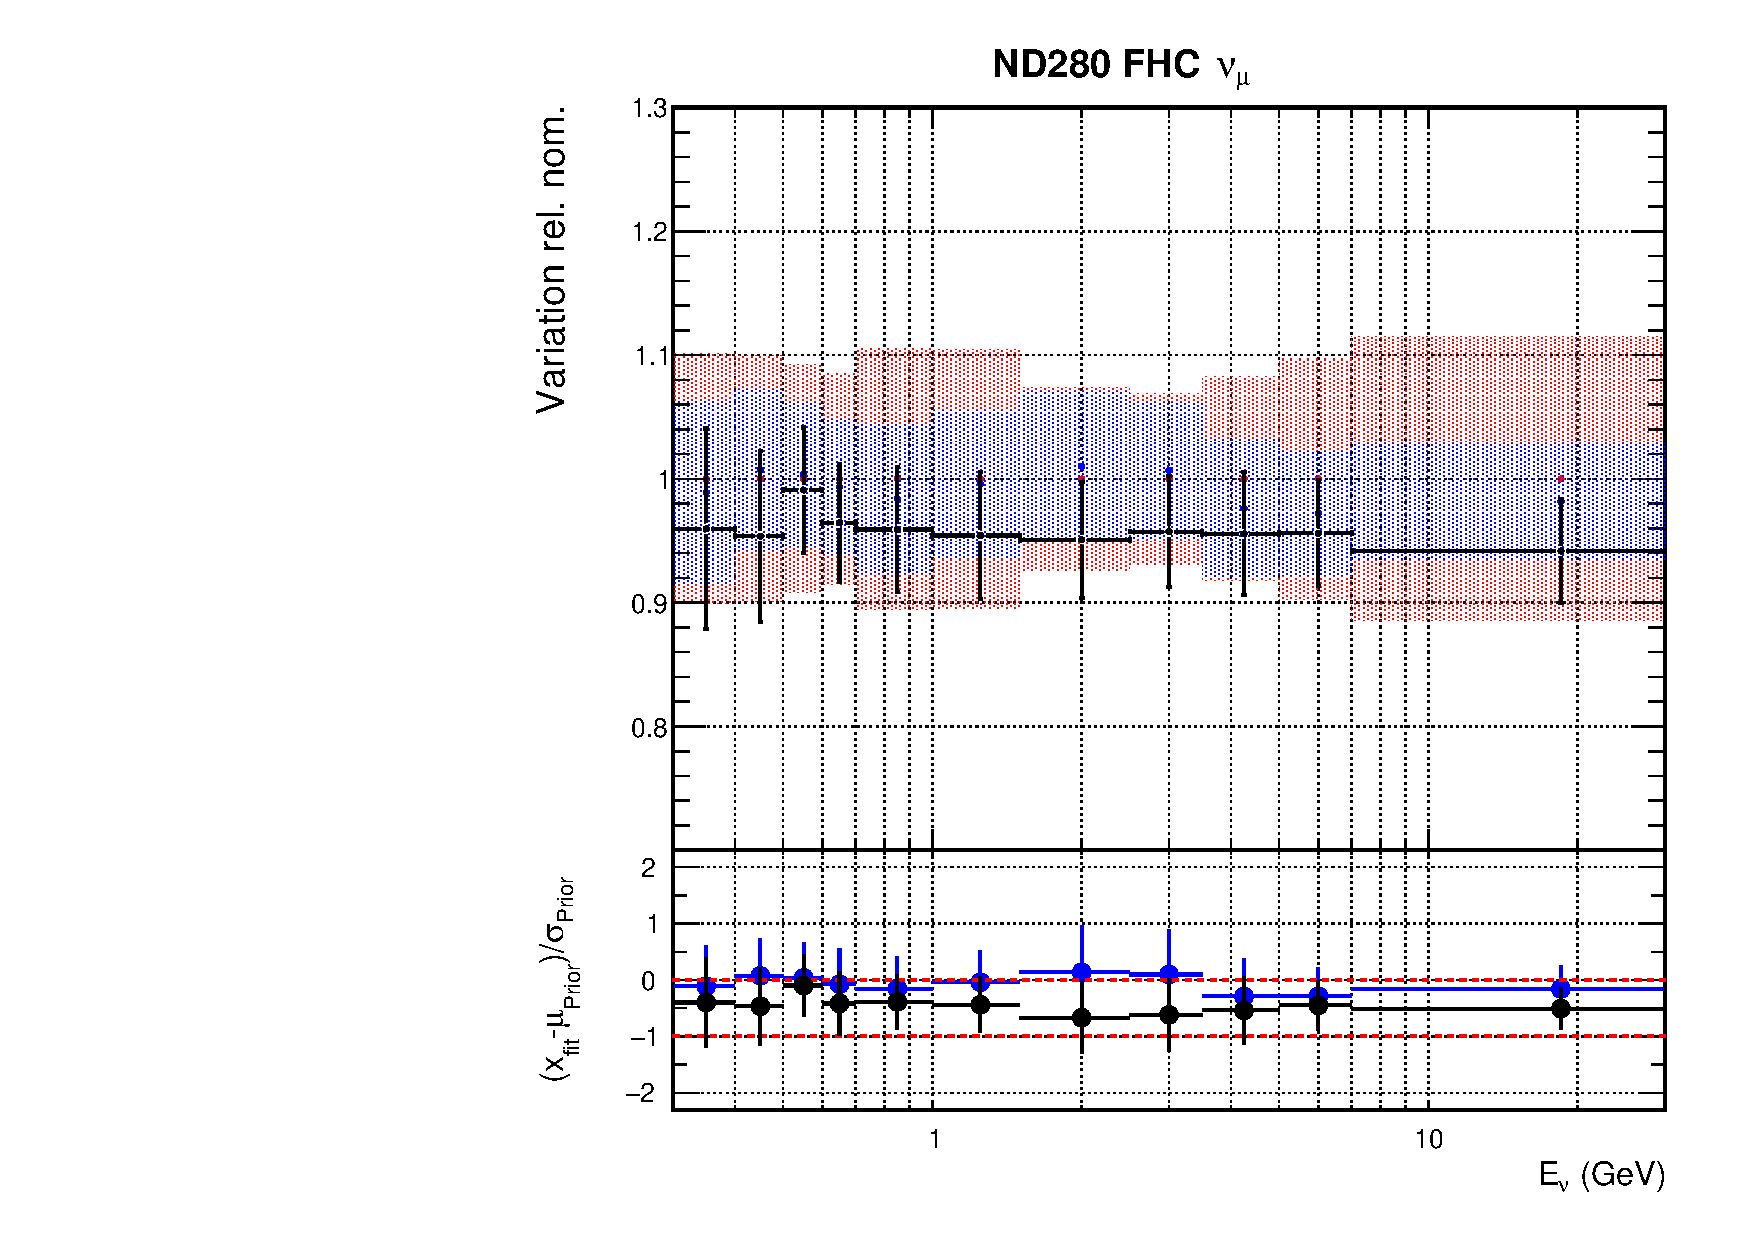
\includegraphics[width=0.95\linewidth]{figs/rhcmpasmvflux0}
  \caption{ND FHC $\nu_{\mu}$}
\end{subfigure}
\begin{subfigure}{0.24\textwidth}
  \centering
  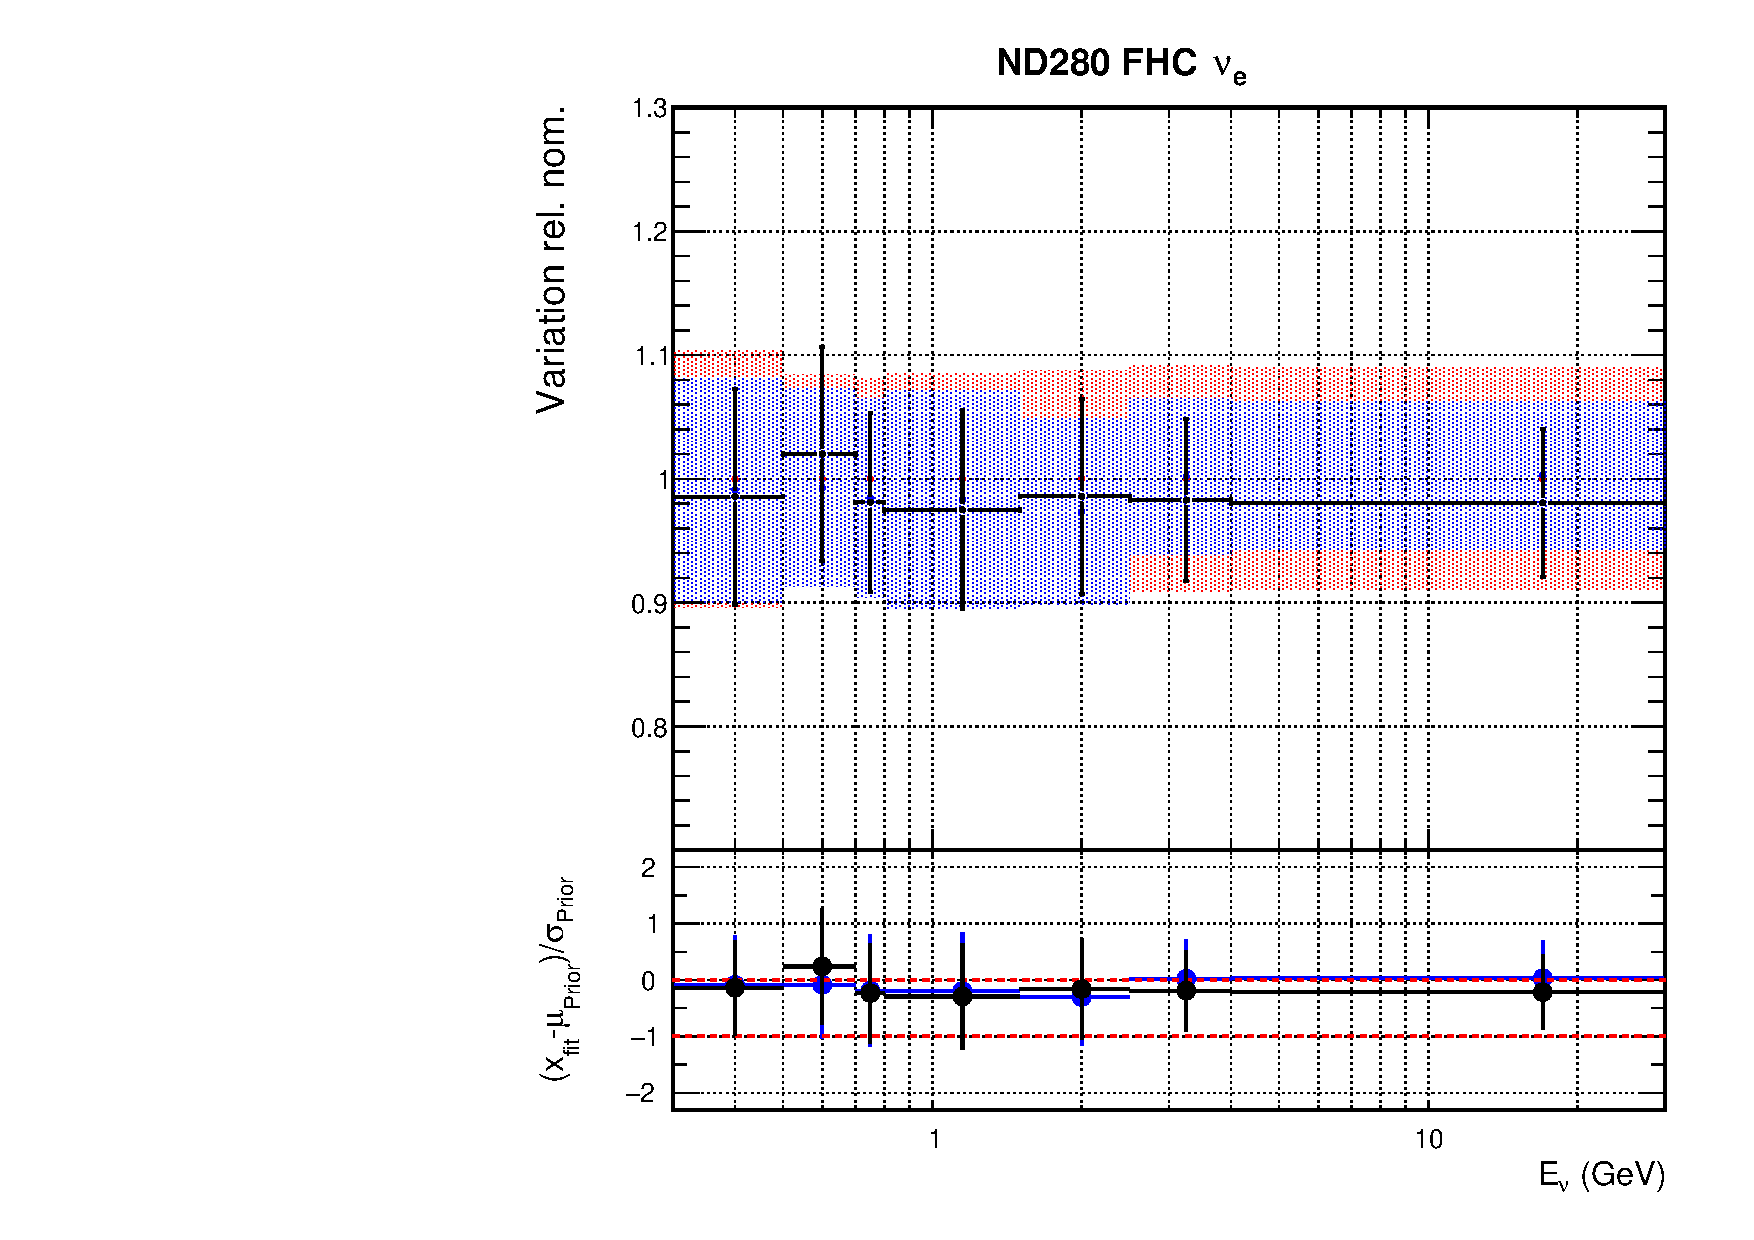
\includegraphics[width=0.95\linewidth]{figs/rhcmpasmvflux1}
  \caption{ND FHC $\nu_e$}
\end{subfigure}
\begin{subfigure}{0.24\textwidth}
  \centering
  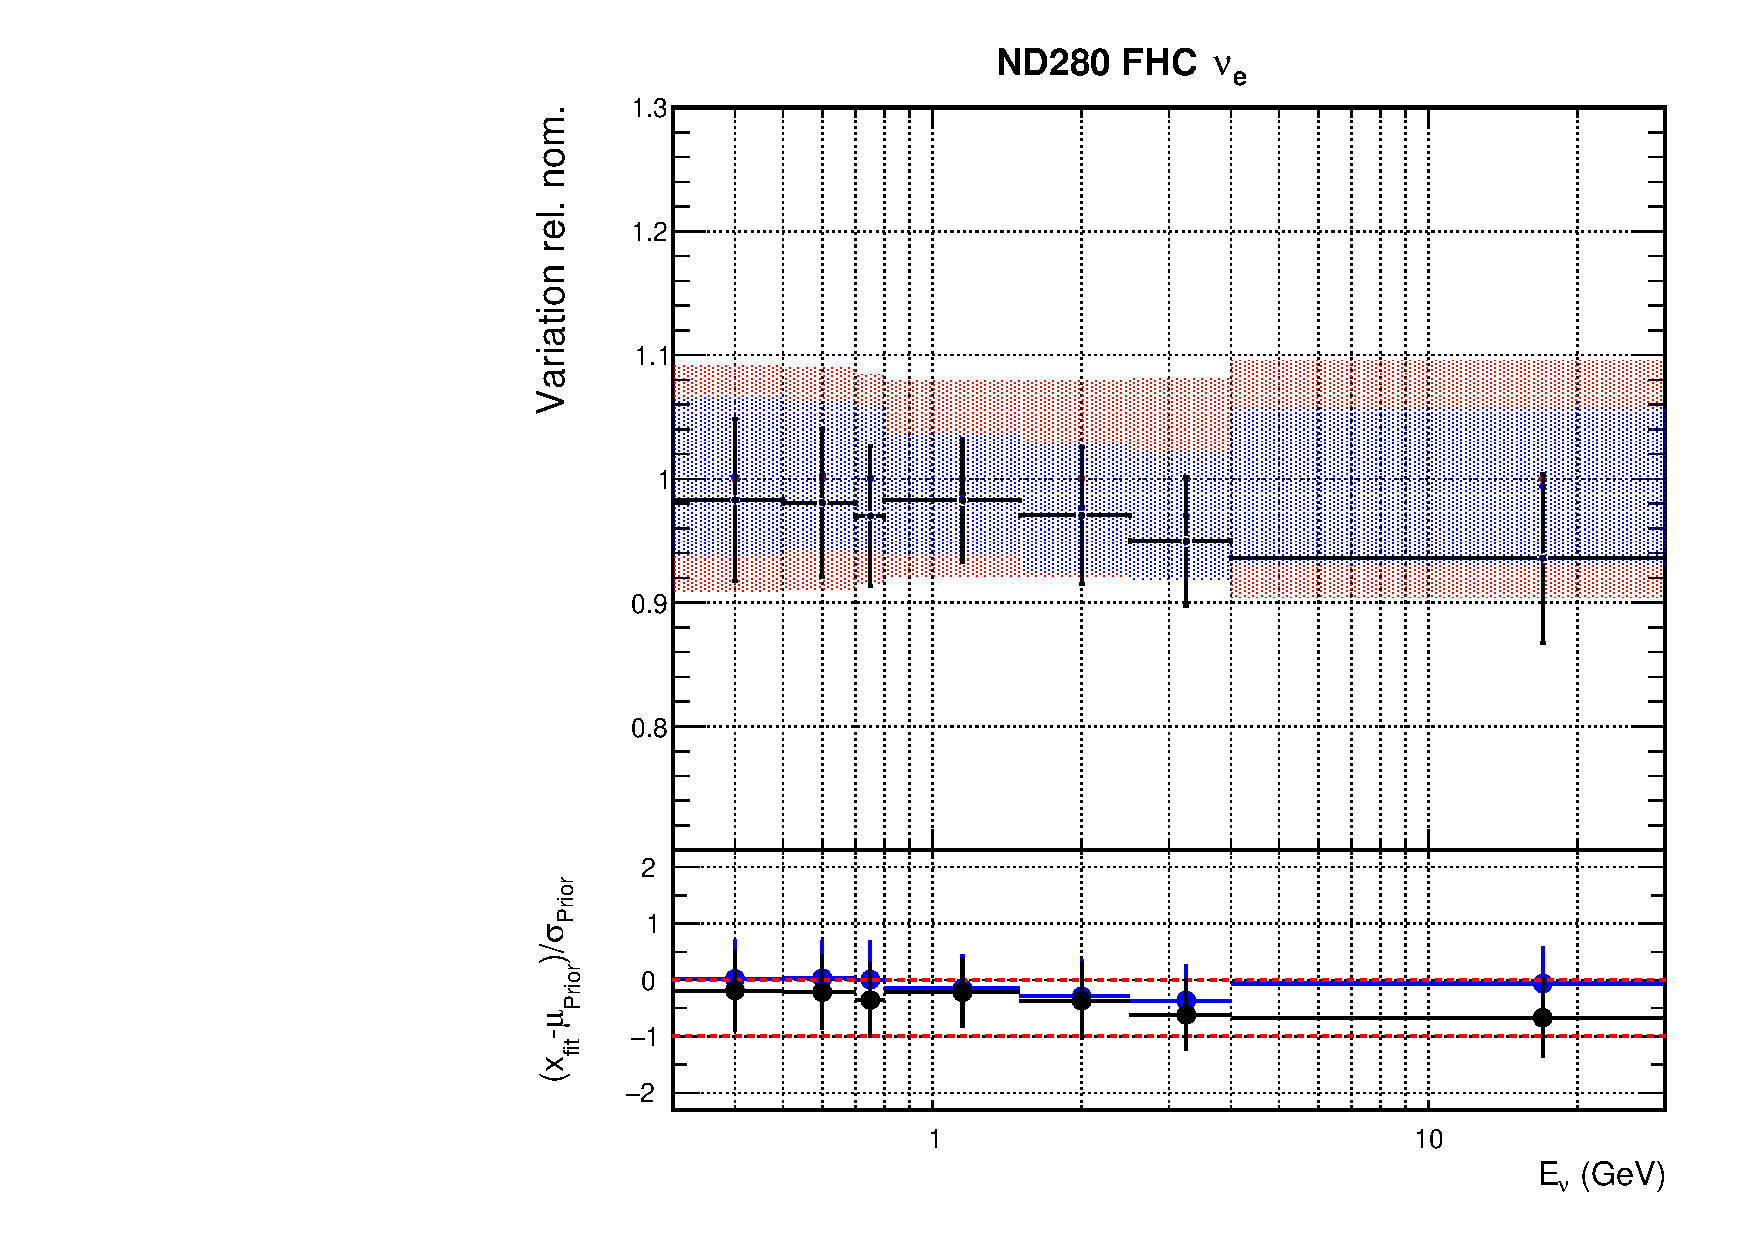
\includegraphics[width=0.95\linewidth]{figs/rhcmpasmvflux2}
  \caption{ND FHC $\bar{\nu_{\mu}}$}
\end{subfigure}
\begin{subfigure}{0.24\textwidth}
  \centering
  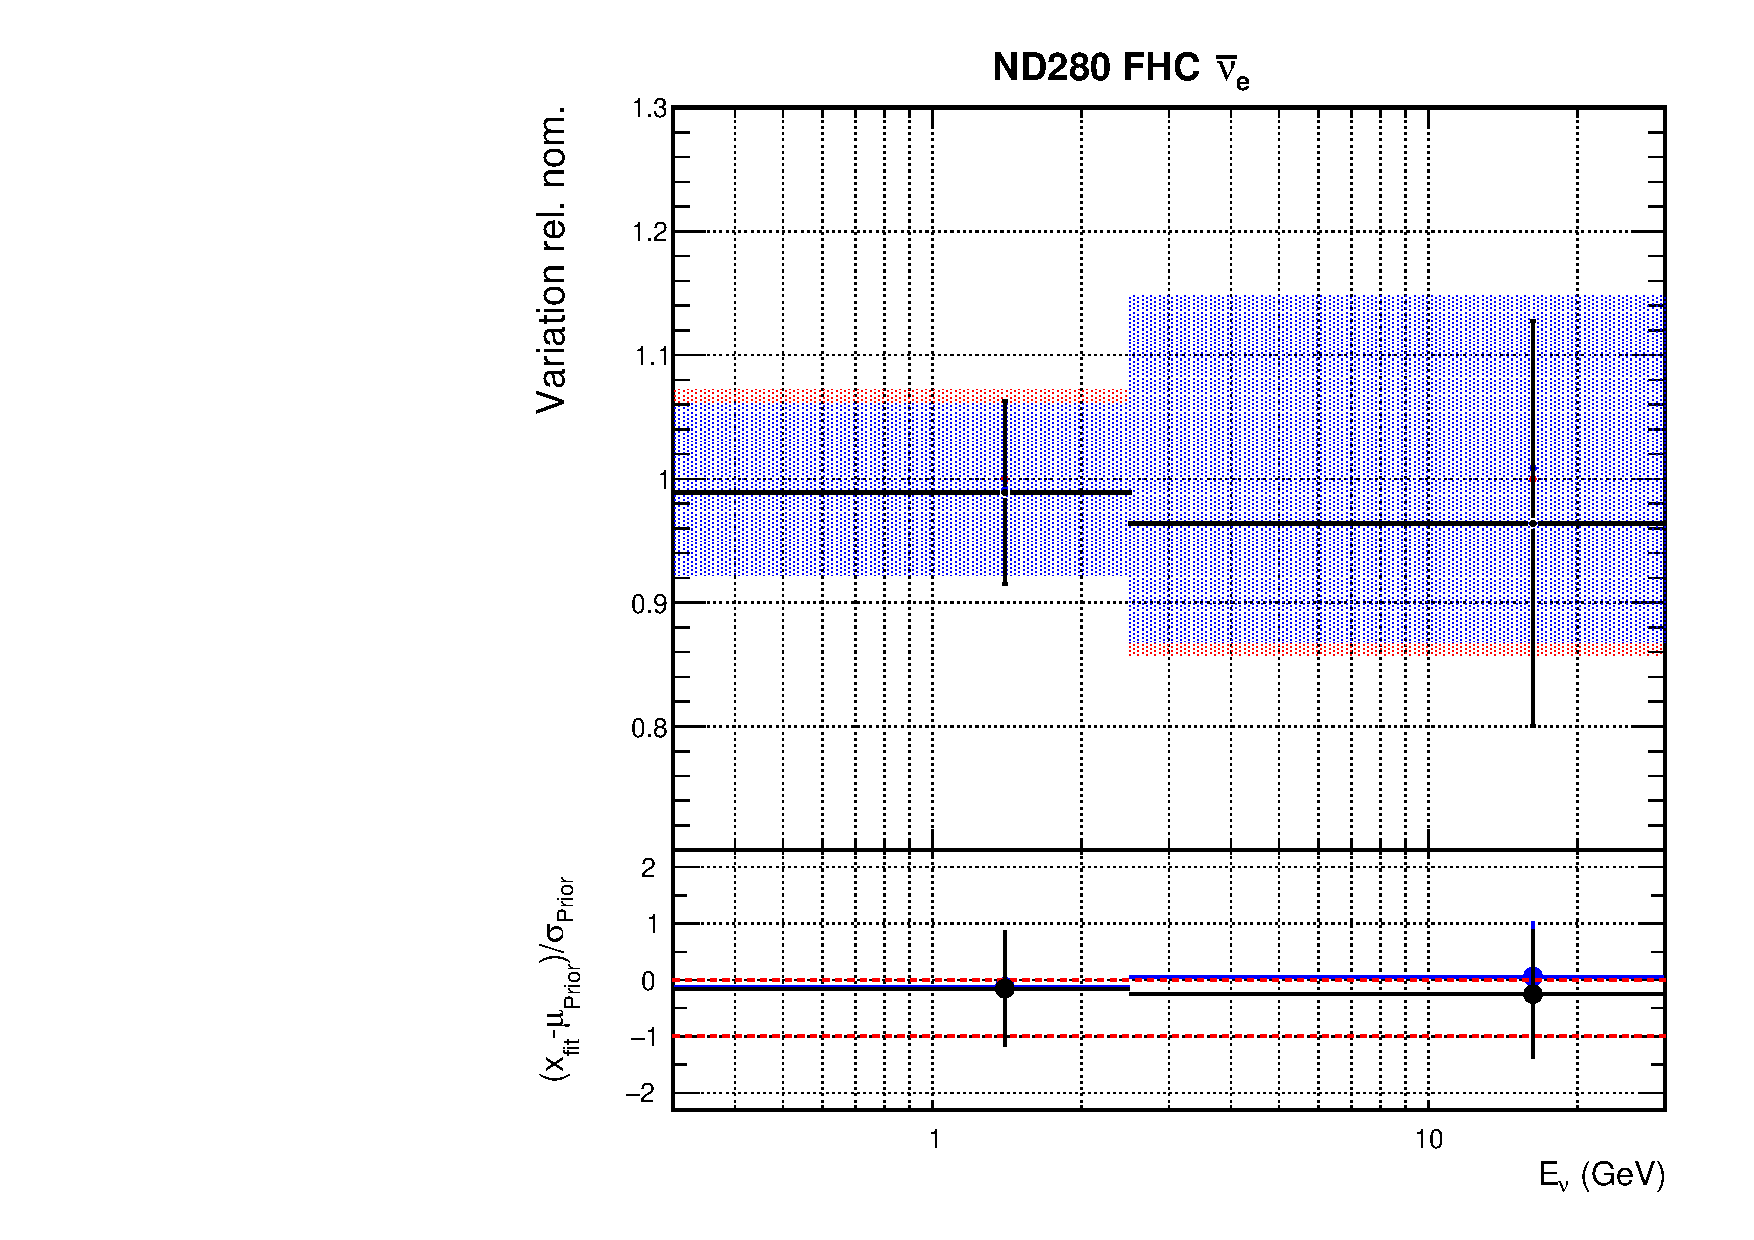
\includegraphics[width=0.95\linewidth]{figs/rhcmpasmvflux3}
  \caption{ND FHC $\bar{\nu_{e}}$}
\end{subfigure}
\begin{subfigure}{0.24\textwidth}
  \centering
  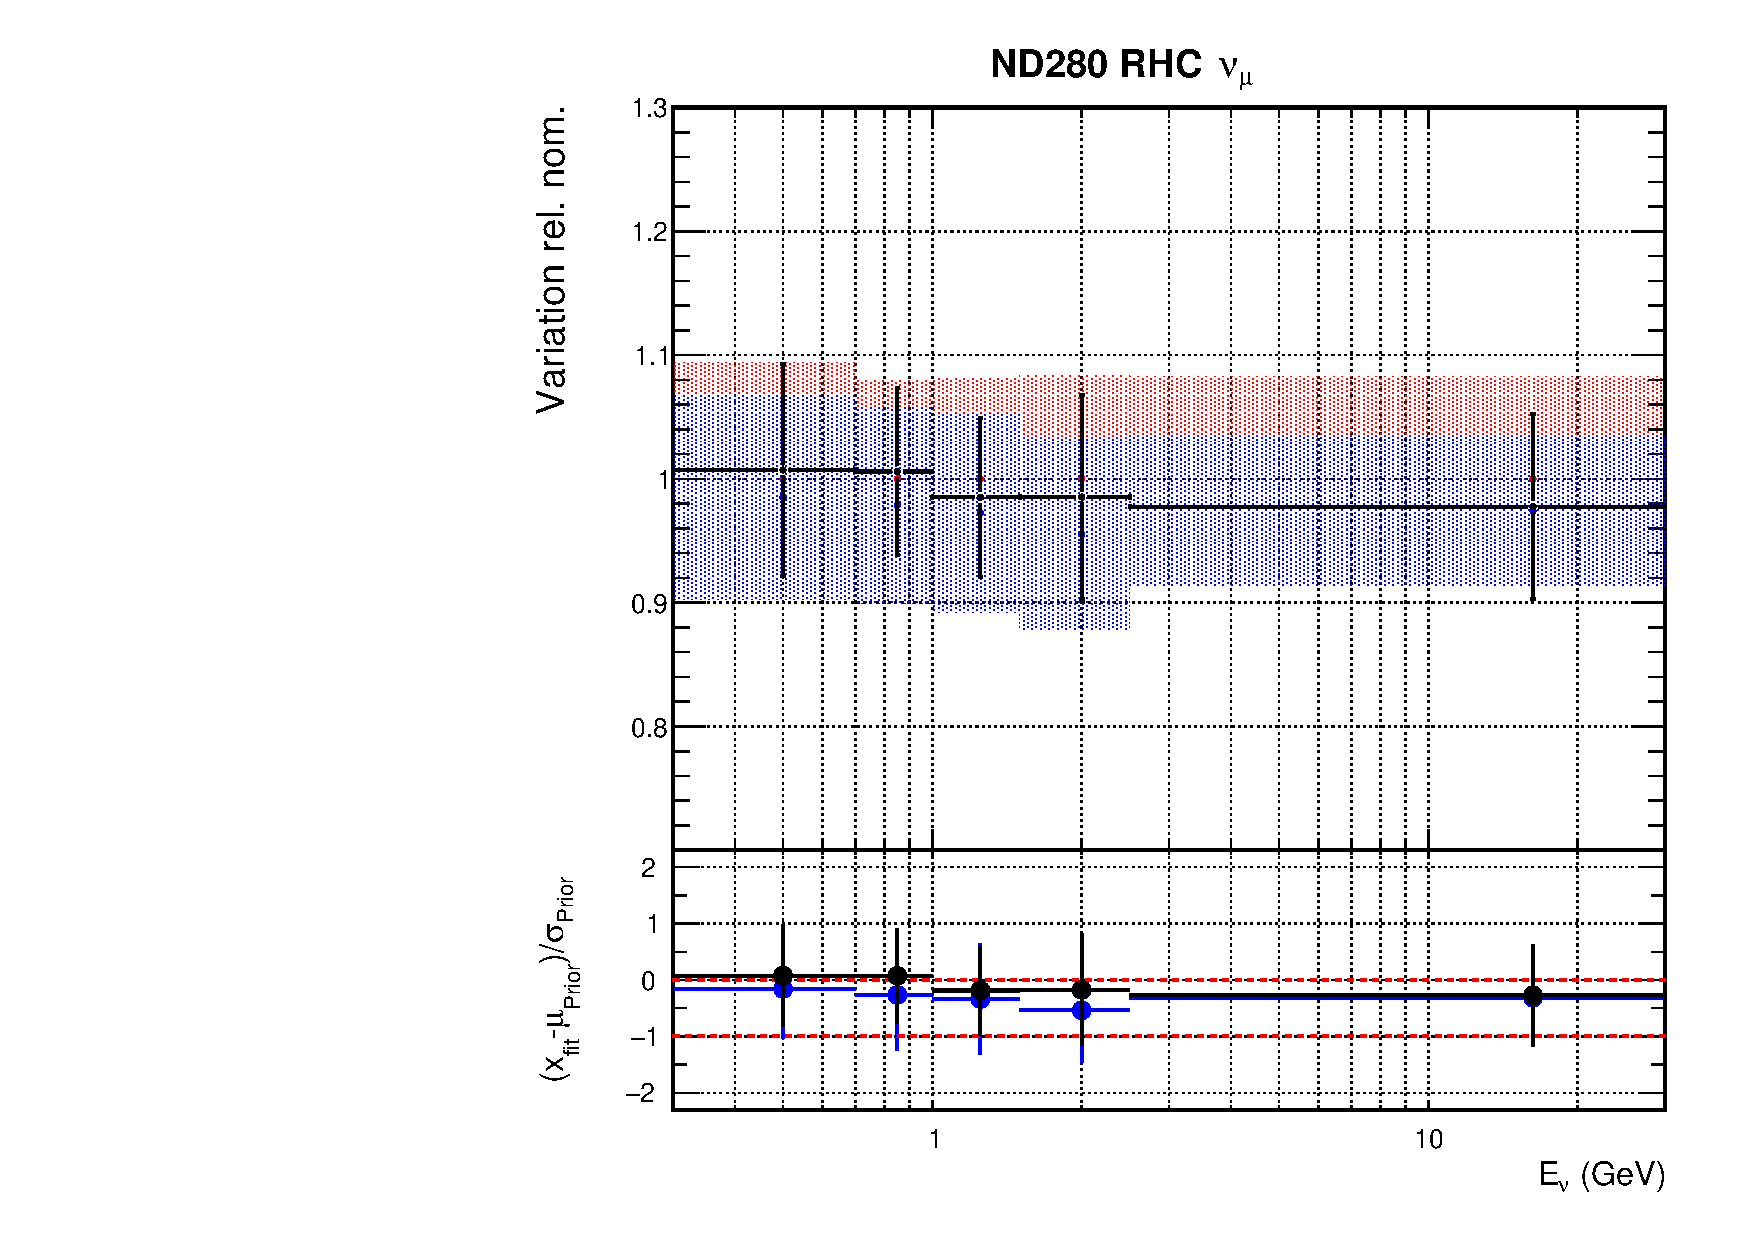
\includegraphics[width=0.95\linewidth]{figs/rhcmpasmvflux4}
  \caption{ND RHC $\bar{\nu_{\mu}}$}
\end{subfigure}
\begin{subfigure}{0.24\textwidth}
  \centering
  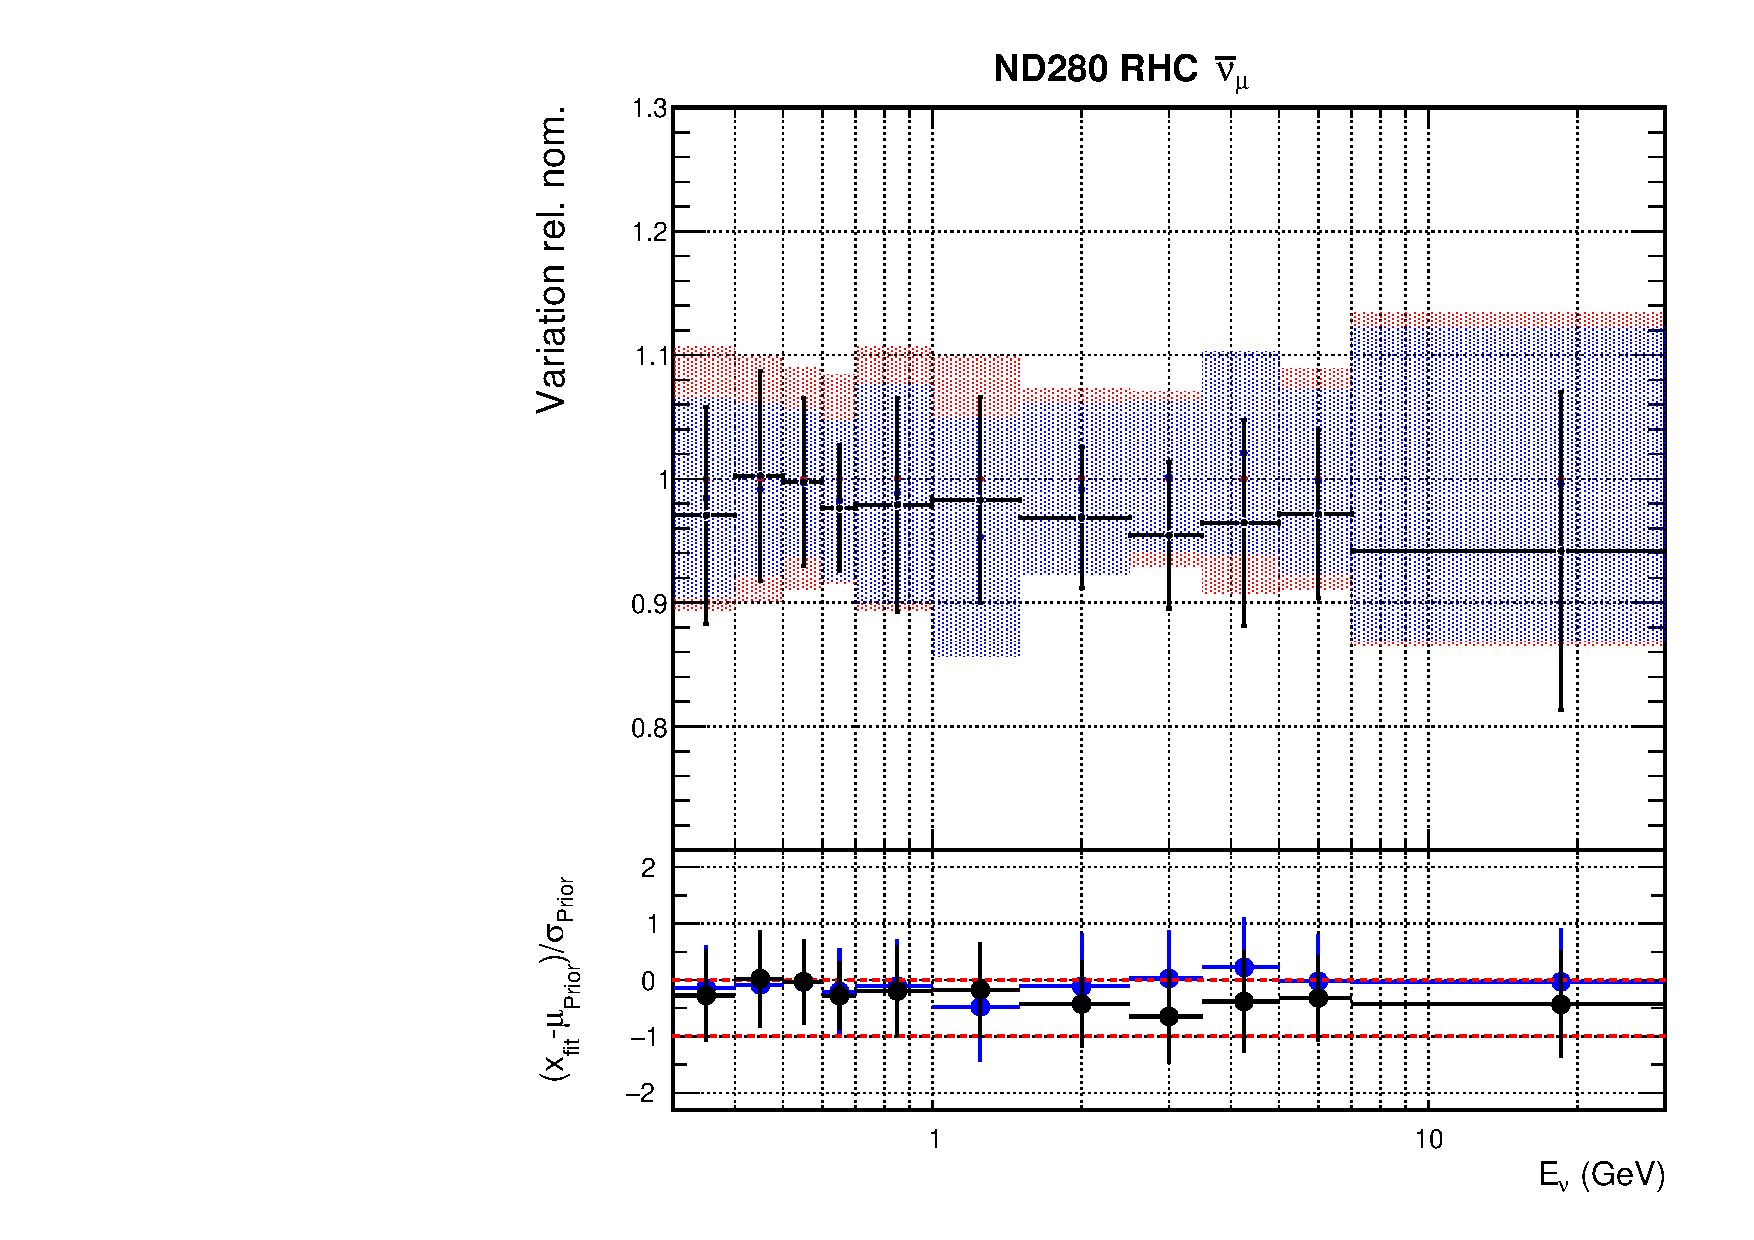
\includegraphics[width=0.95\linewidth]{figs/rhcmpasmvflux5}
  \caption{ND RHC $\bar{\nu_{e}}$}
\end{subfigure}
\begin{subfigure}{0.24\textwidth}
  \centering
  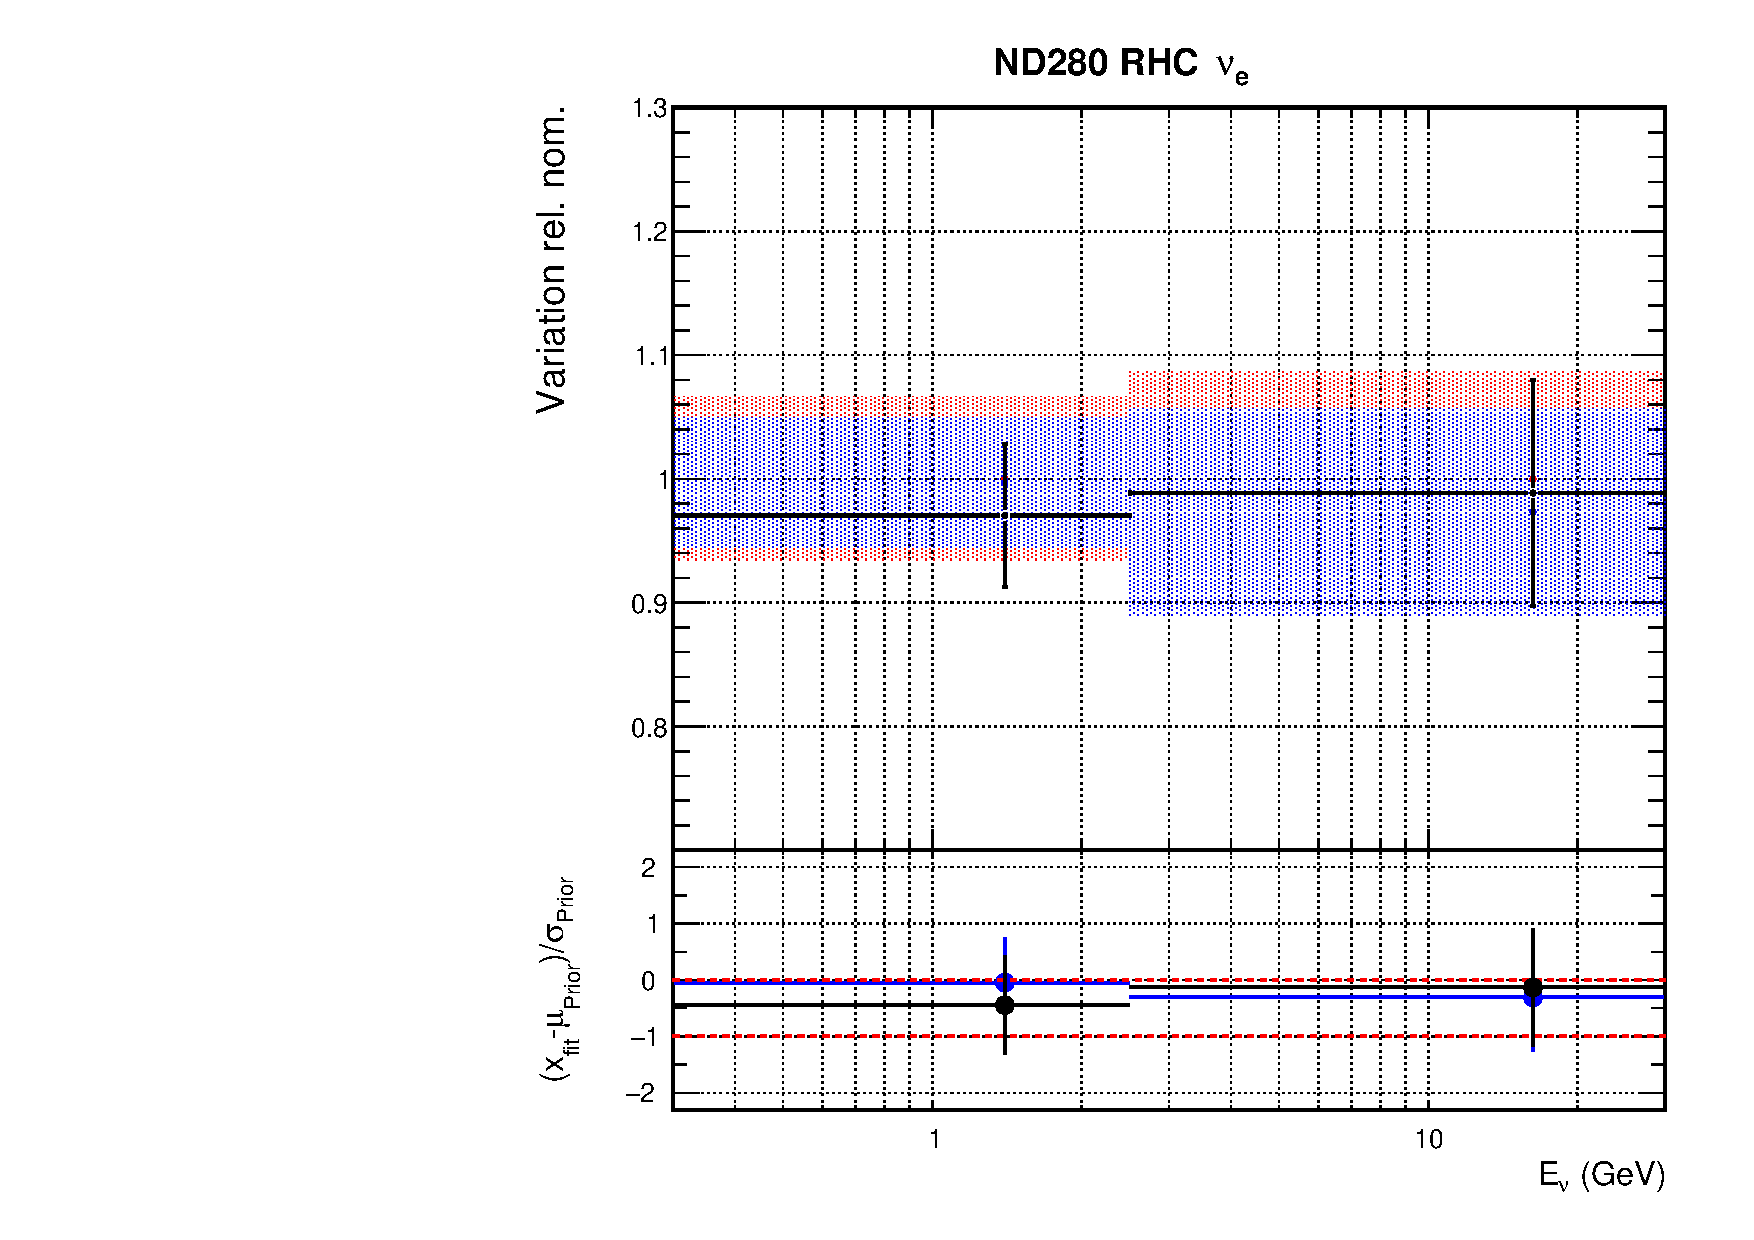
\includegraphics[width=0.95\linewidth]{figs/rhcmpasmvflux6}
  \caption{ND RHC $\nu_{\mu}$}
\end{subfigure}
\vspace{15mm}
\begin{subfigure}{0.24\textwidth}
  \centering
  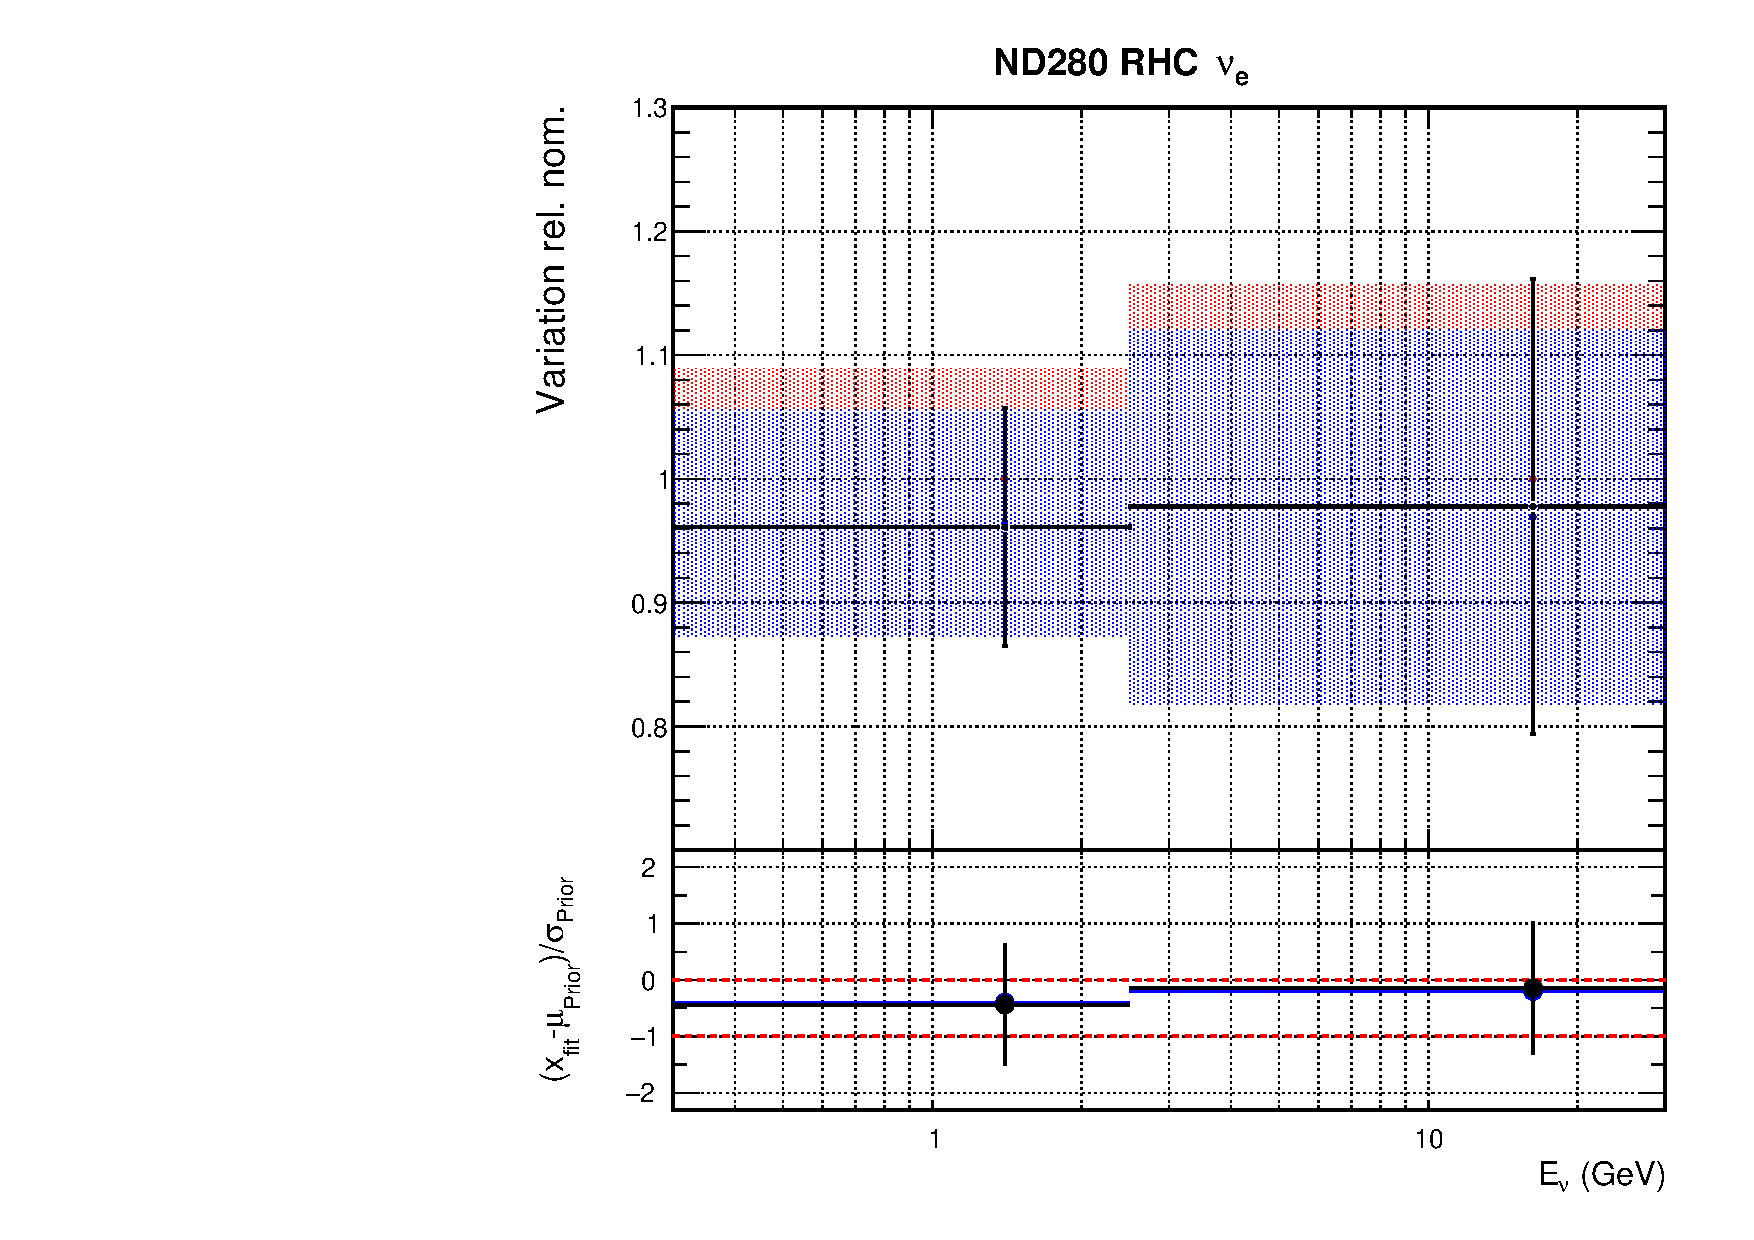
\includegraphics[width=0.95\linewidth]{figs/rhcmpasmvflux7}
  \caption{ND RHC $\nu_e$}
\end{subfigure}
\begin{subfigure}{0.24\textwidth}
  \centering
  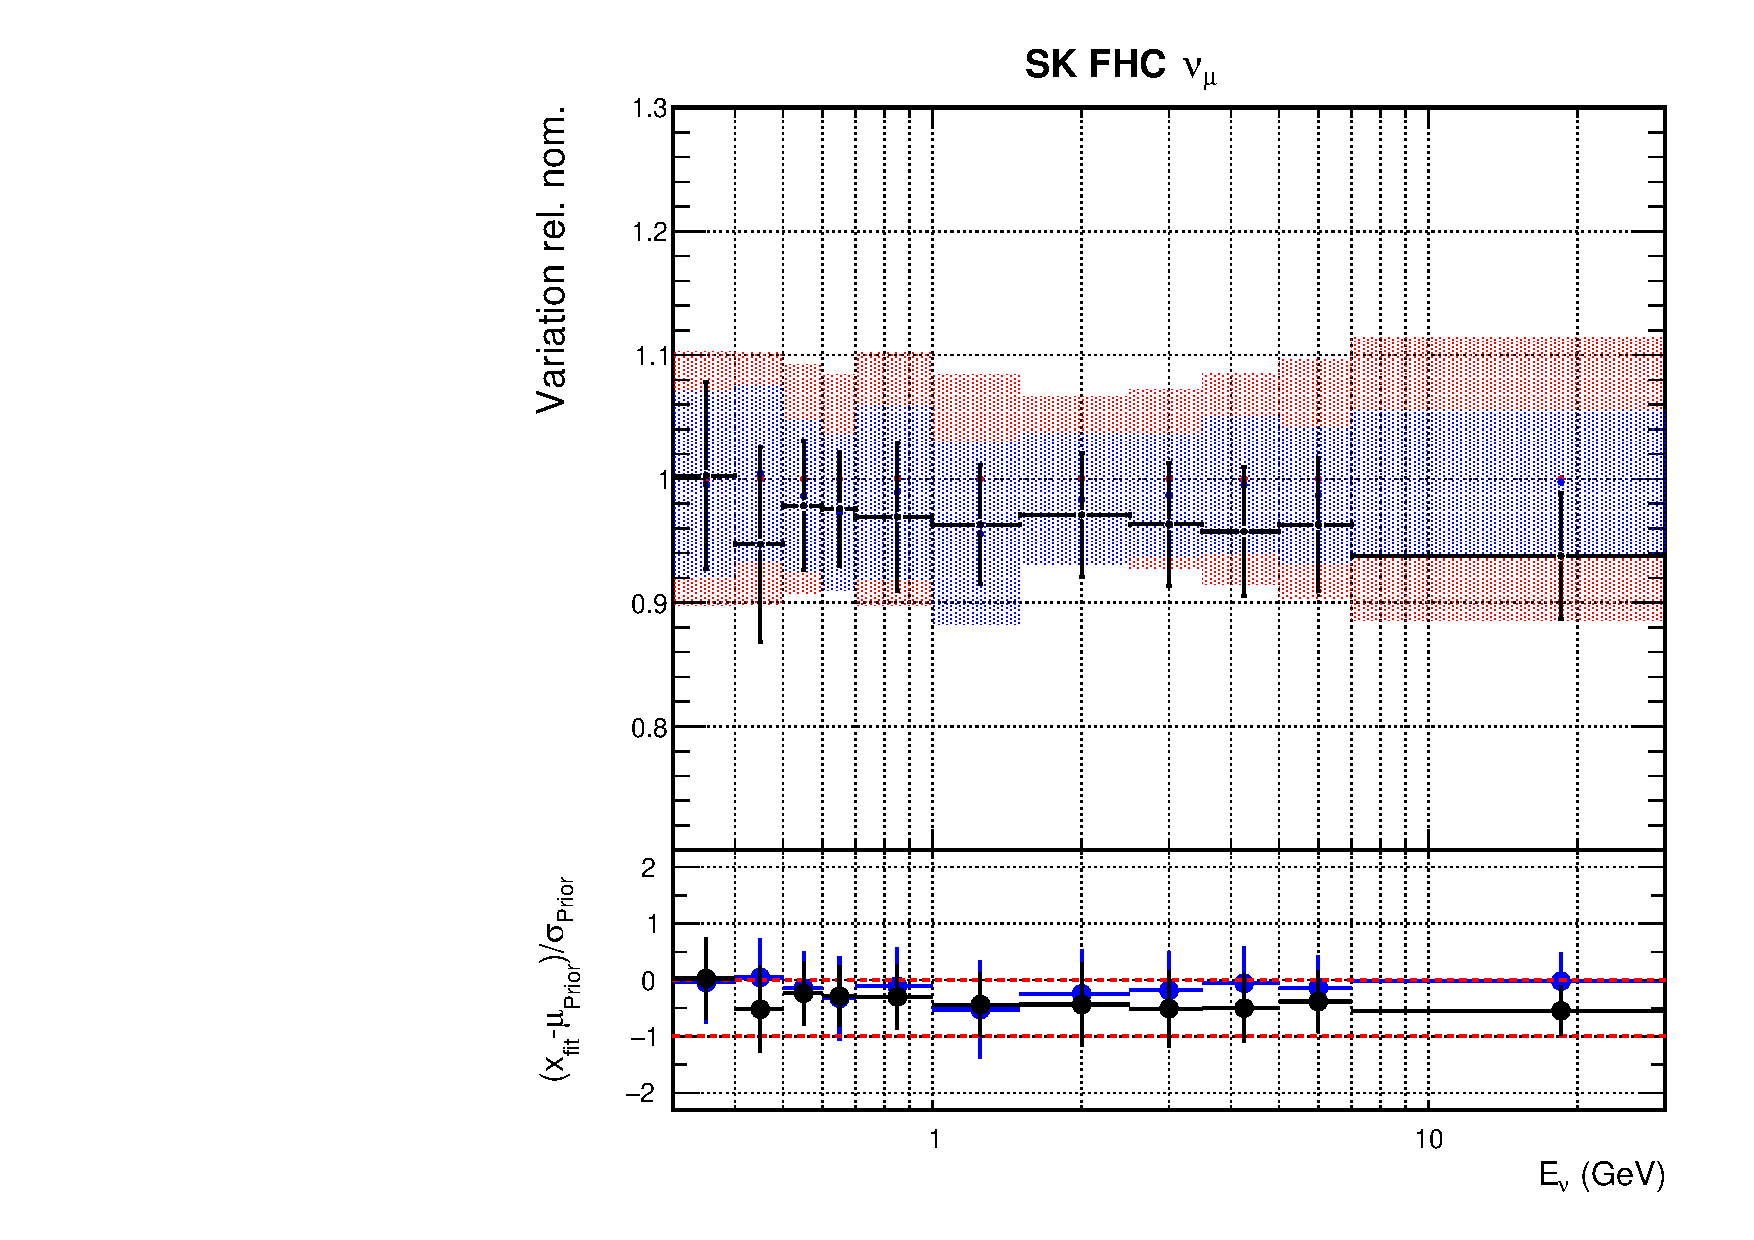
\includegraphics[width=0.95\linewidth]{figs/rhcmpasmvflux8}
  \caption{SK FHC $\nu_{\mu}$}
\end{subfigure}
\begin{subfigure}{0.24\textwidth}
  \centering
  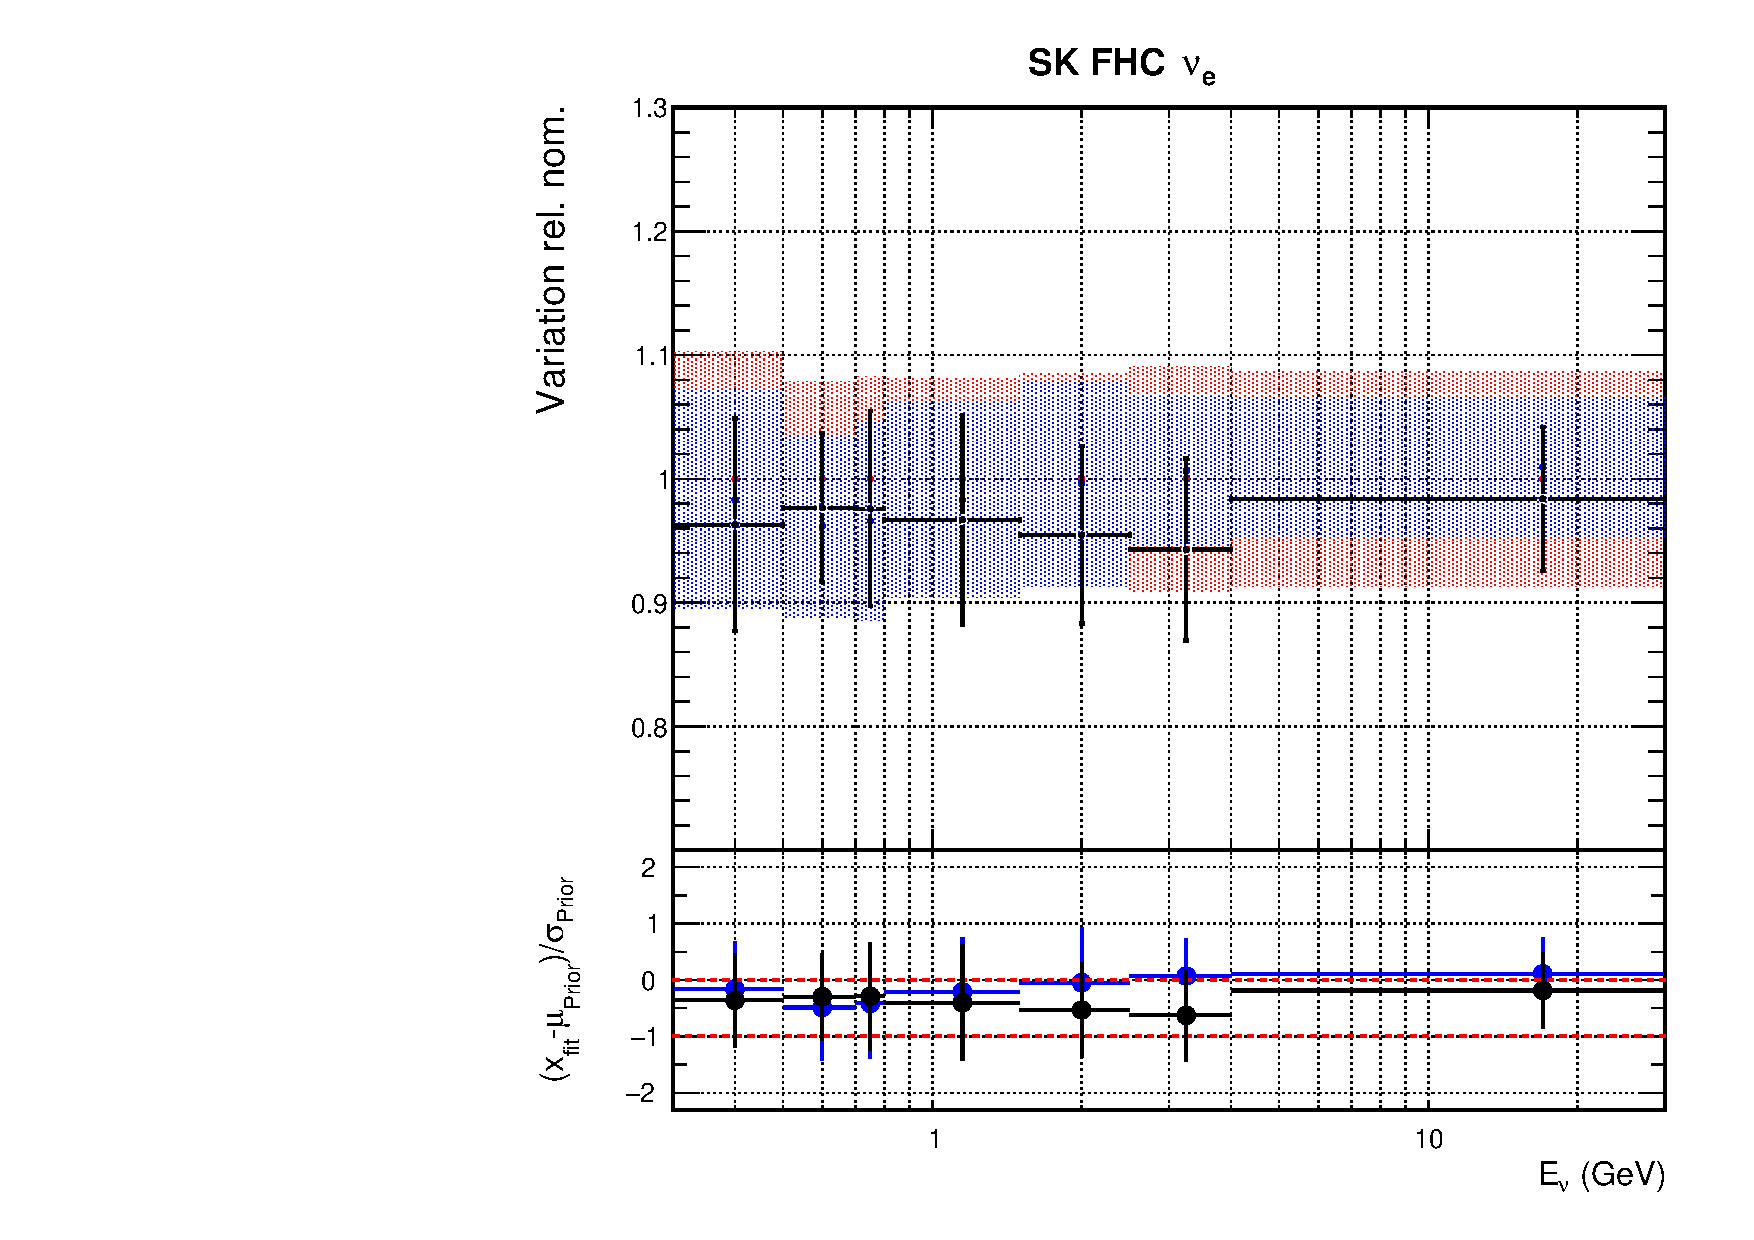
\includegraphics[width=0.95\linewidth]{figs/rhcmpasmvflux9}
  \caption{SK FHC $\nu_e$}
\end{subfigure}
\begin{subfigure}{0.24\textwidth}
  \centering
  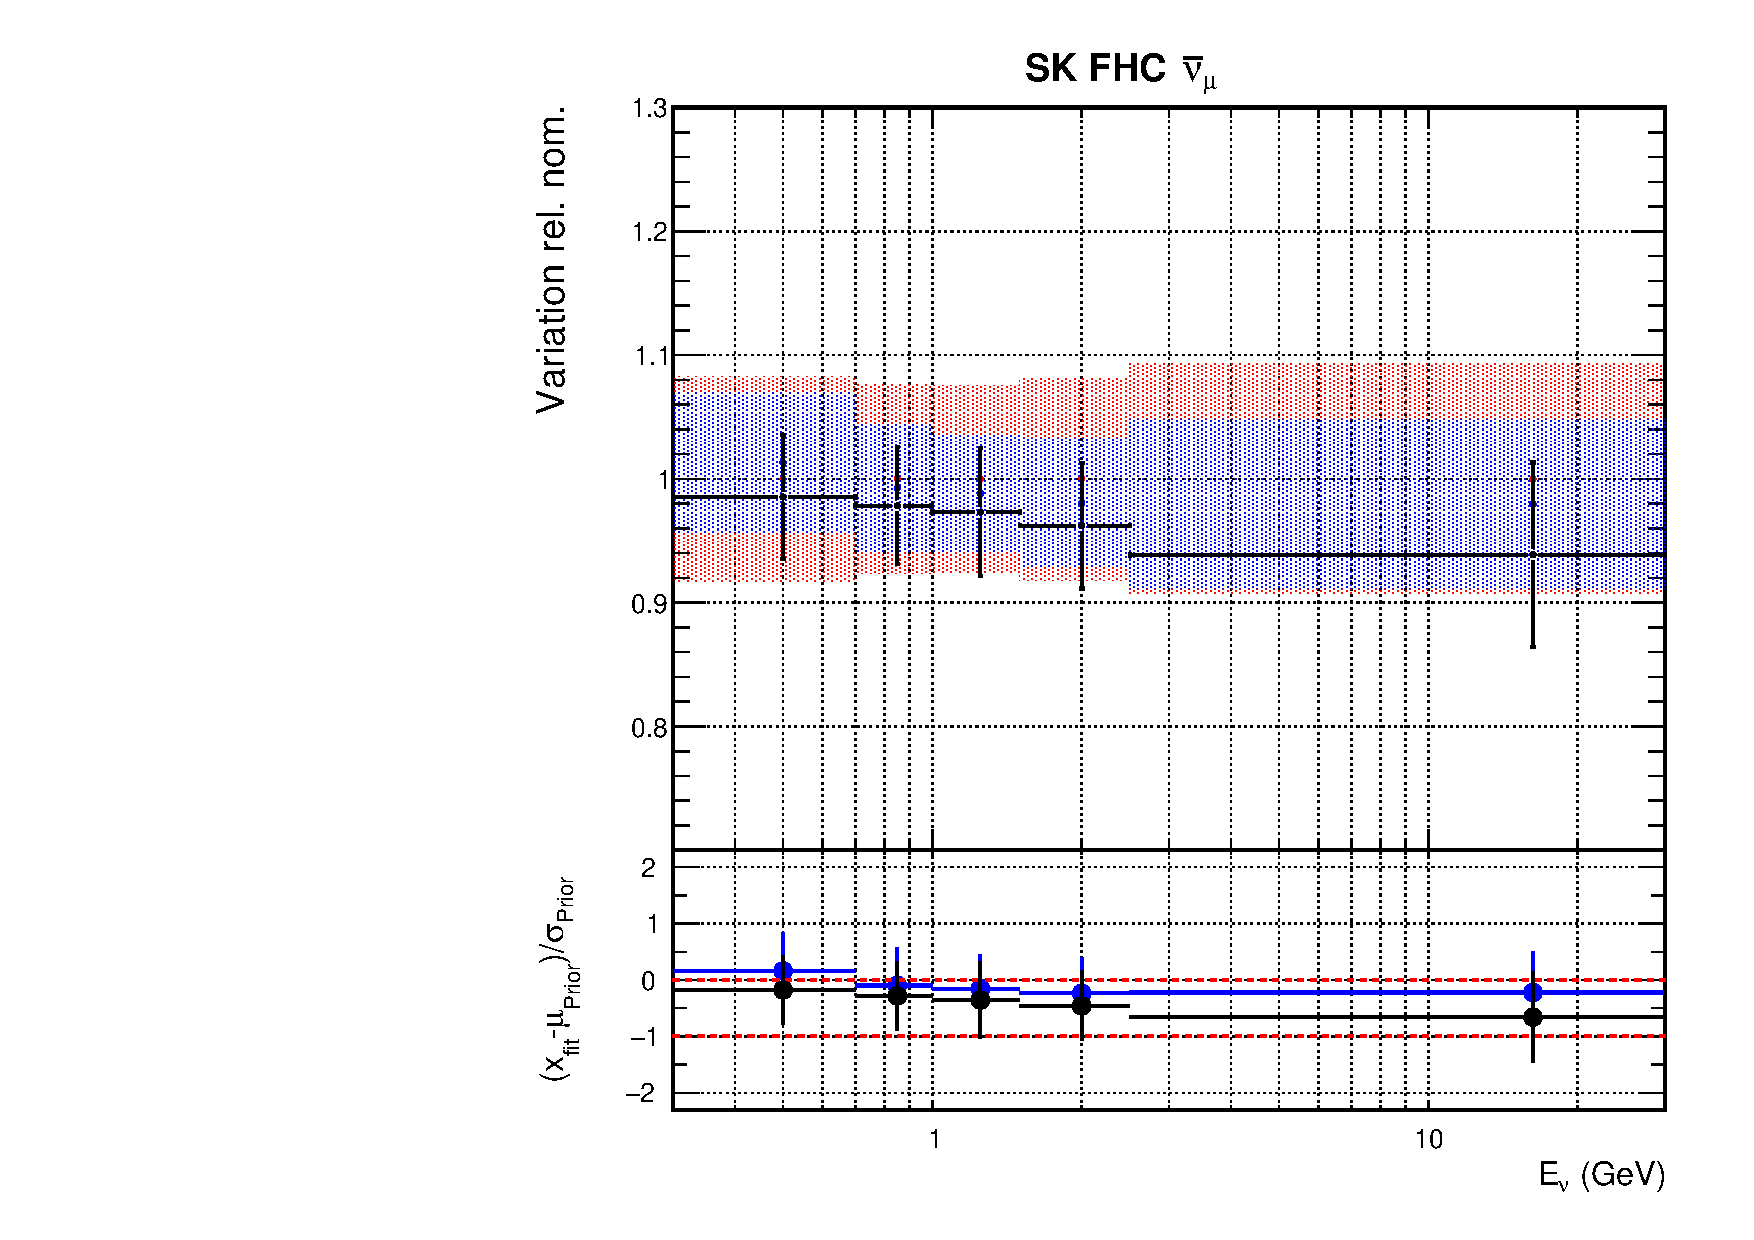
\includegraphics[width=0.95\linewidth]{figs/rhcmpasmvflux10}
  \caption{SK FHC $\bar{\nu_{\mu}}$}
\end{subfigure}
\begin{subfigure}{0.24\textwidth}
  \centering
  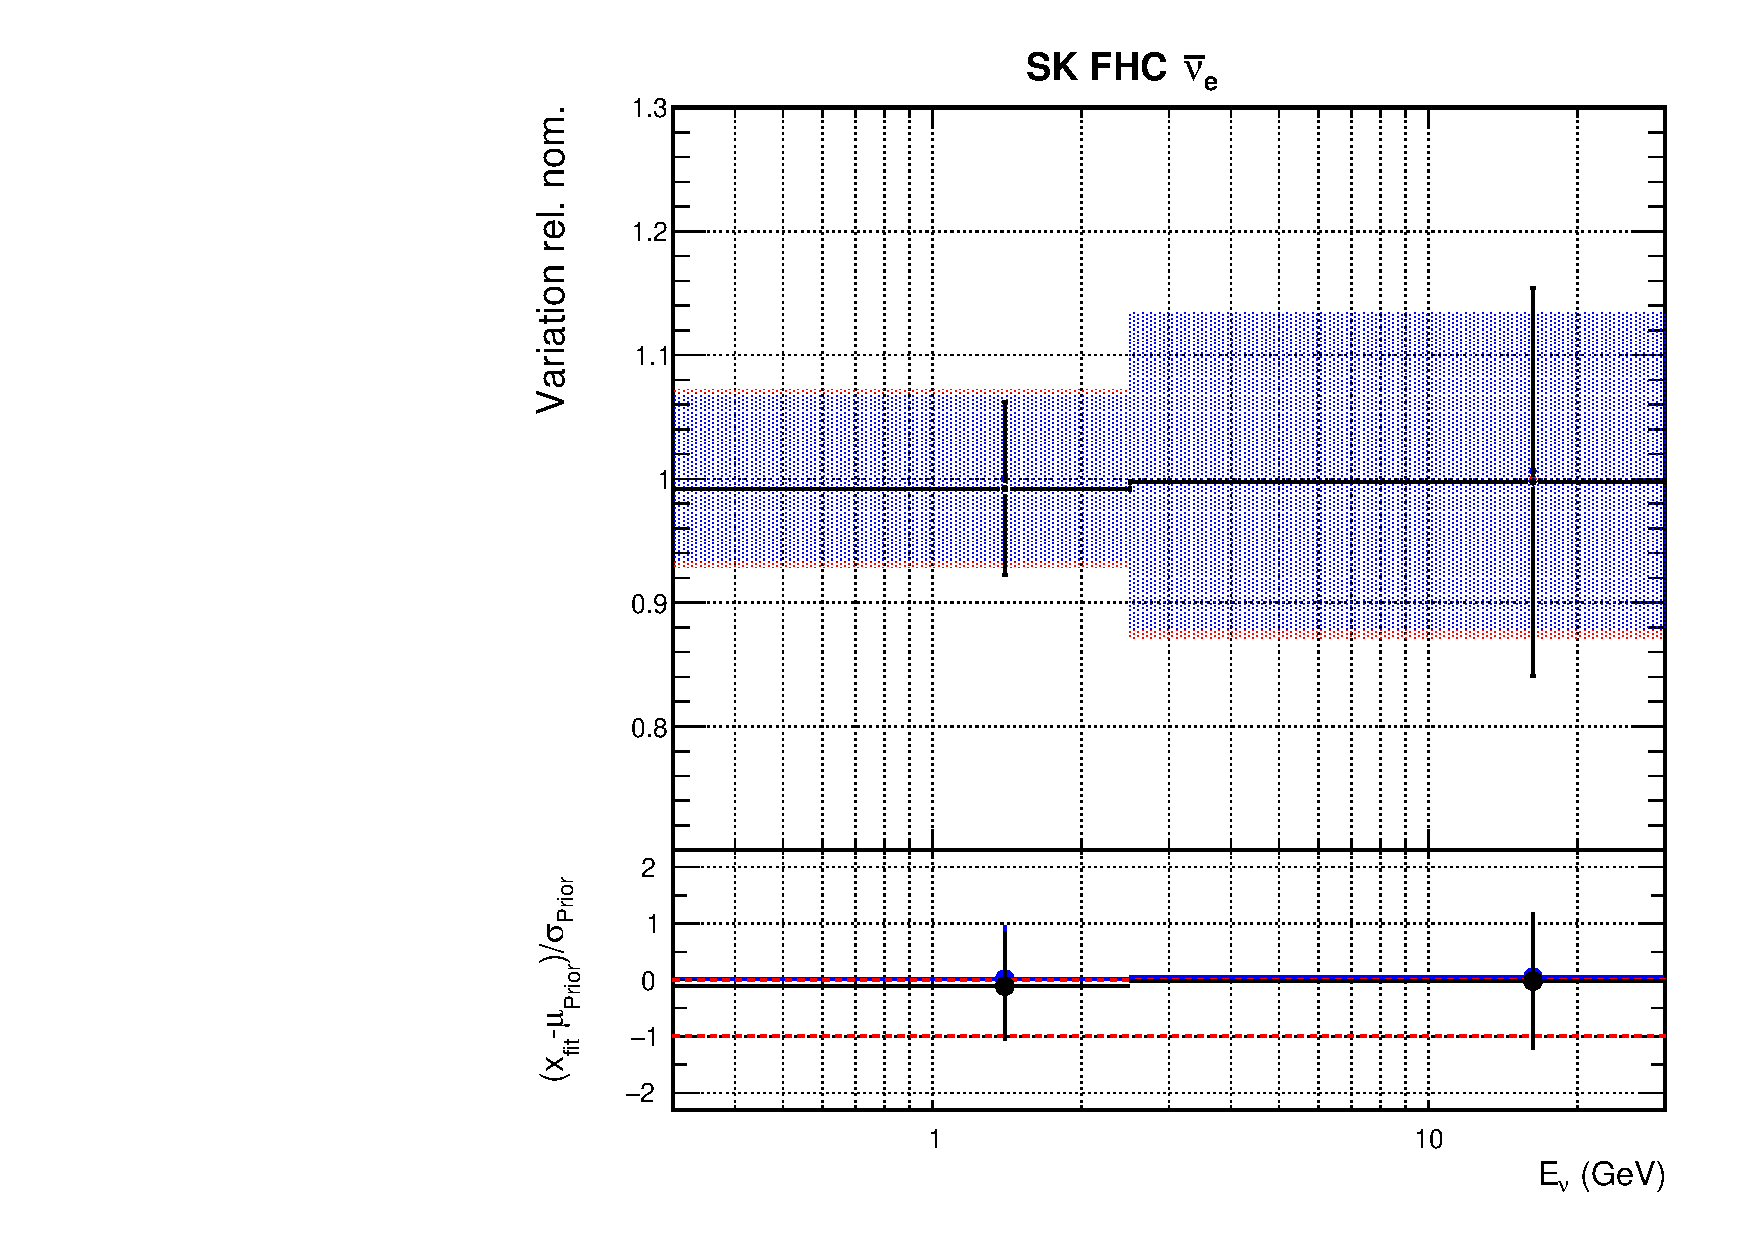
\includegraphics[width=0.95\linewidth]{figs/rhcmpasmvflux11}
  \caption{SK FHC $\bar{\nu_e}$}
\end{subfigure}
\begin{subfigure}{0.24\textwidth}
  \centering
  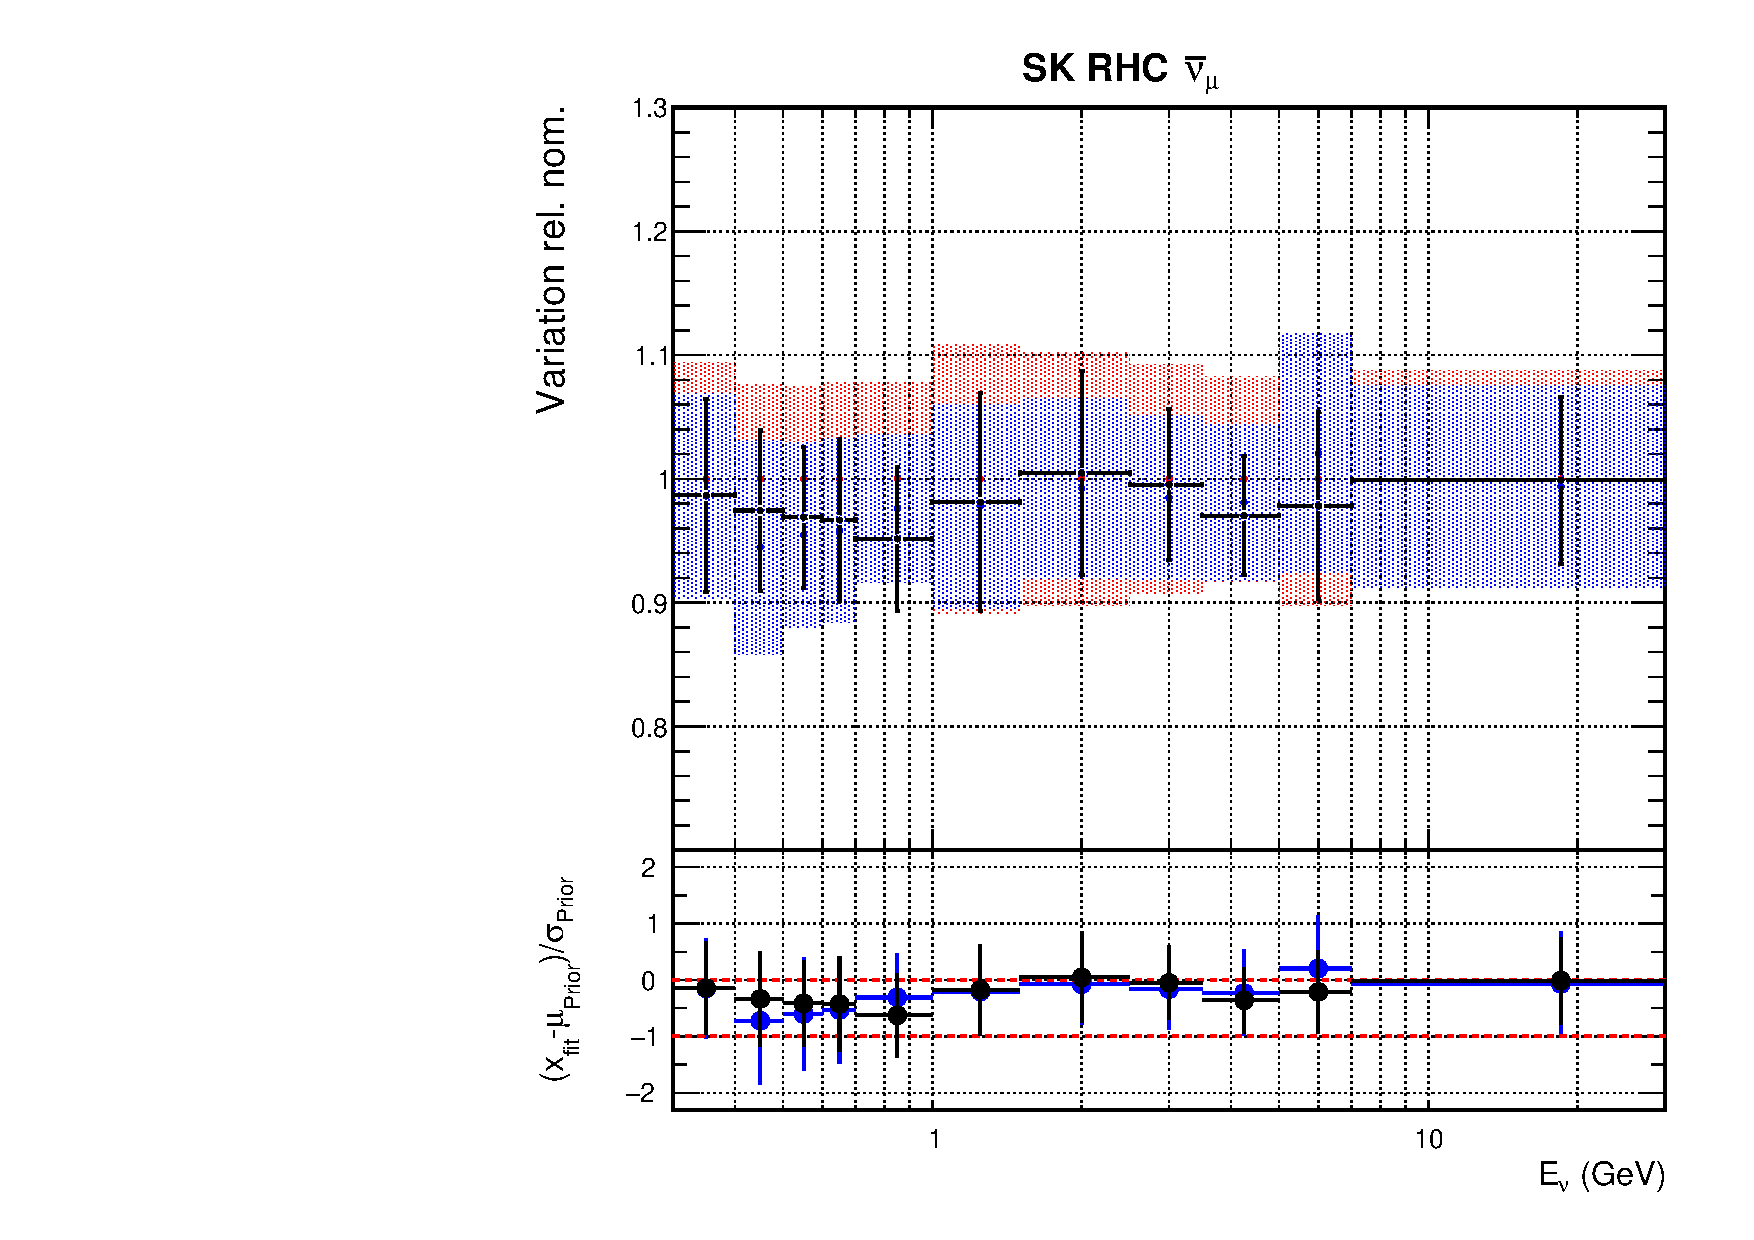
\includegraphics[width=0.95\linewidth]{figs/rhcmpasmvflux12}
  \caption{SK RHC $\bar{\nu_{\mu}}$}
\end{subfigure}
\begin{subfigure}{0.24\textwidth}
  \centering
  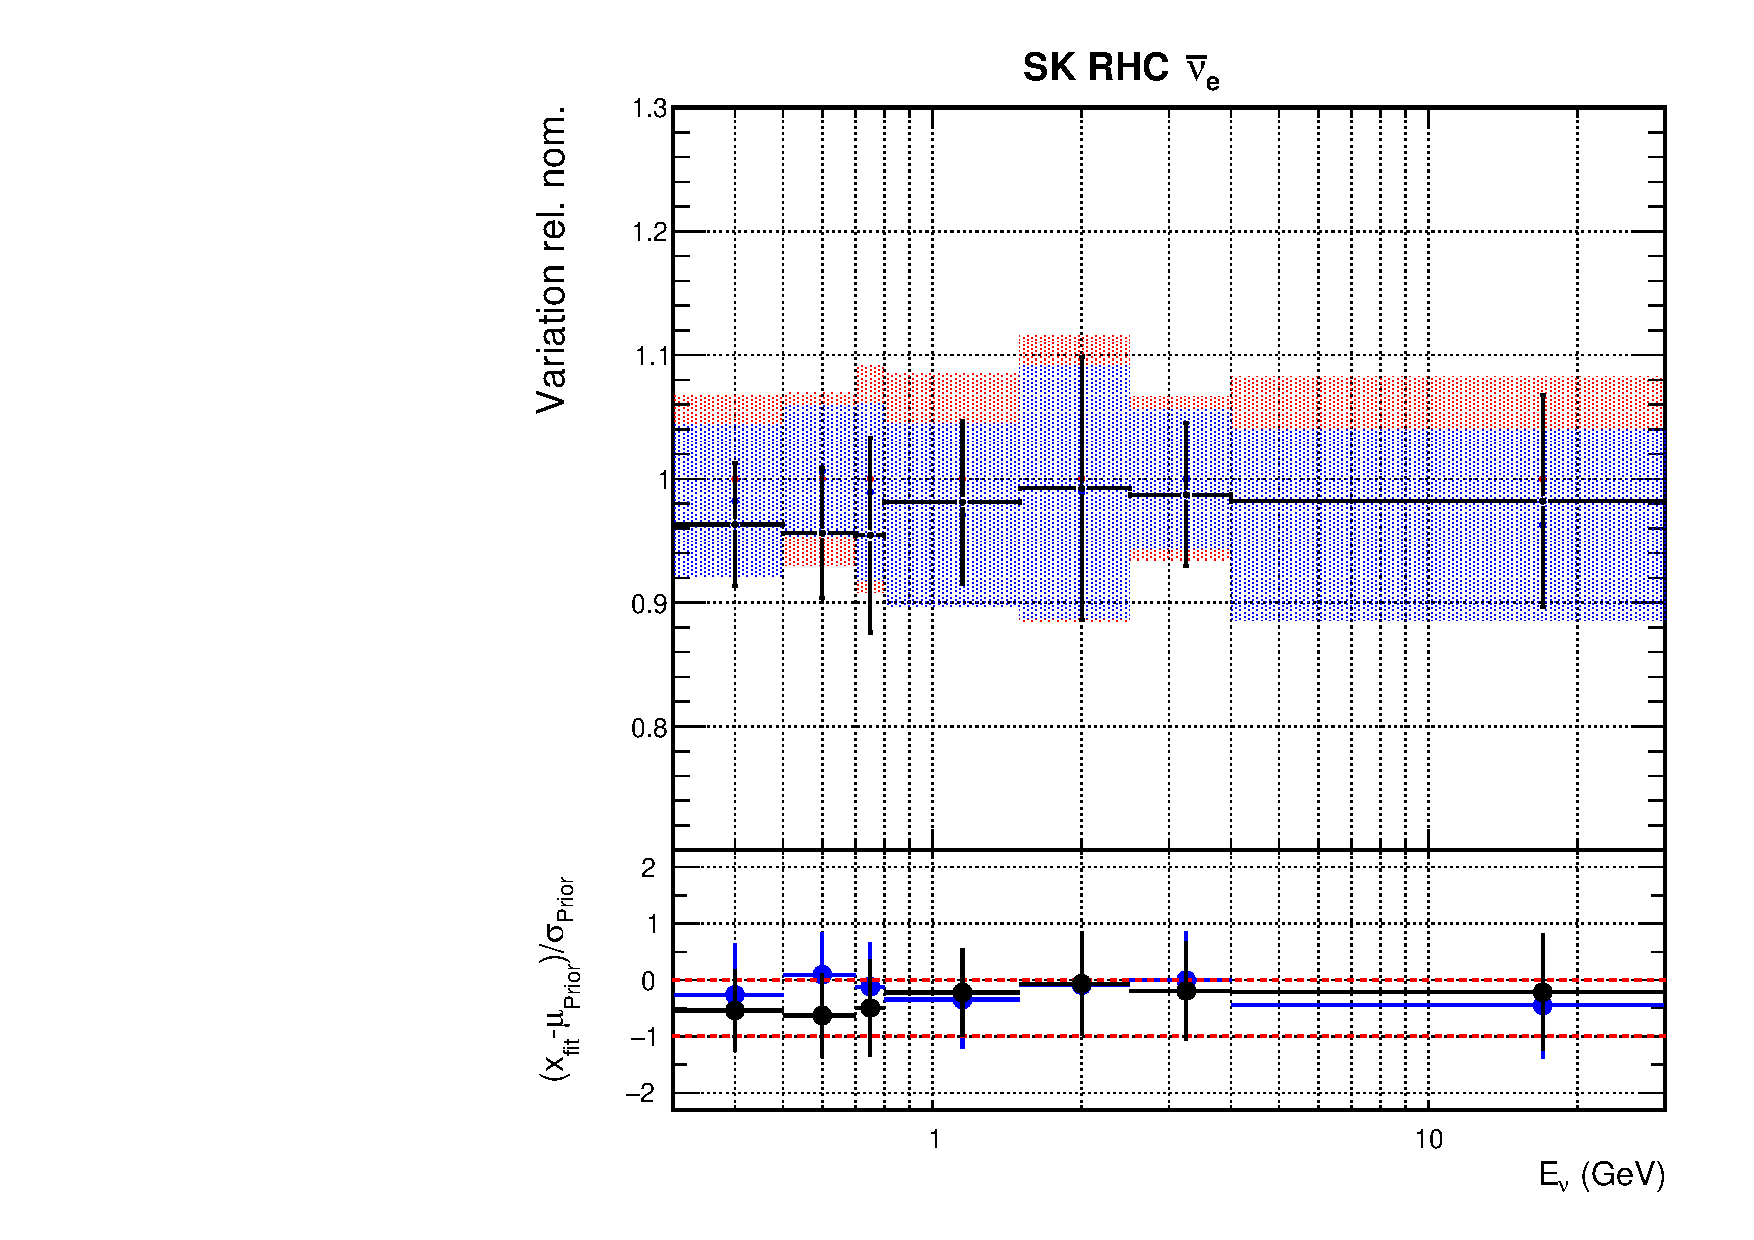
\includegraphics[width=0.95\linewidth]{figs/rhcmpasmvflux13}
  \caption{SK RHC $\bar{\nu_e}$}
\end{subfigure}
\begin{subfigure}{0.24\textwidth}
  \centering
  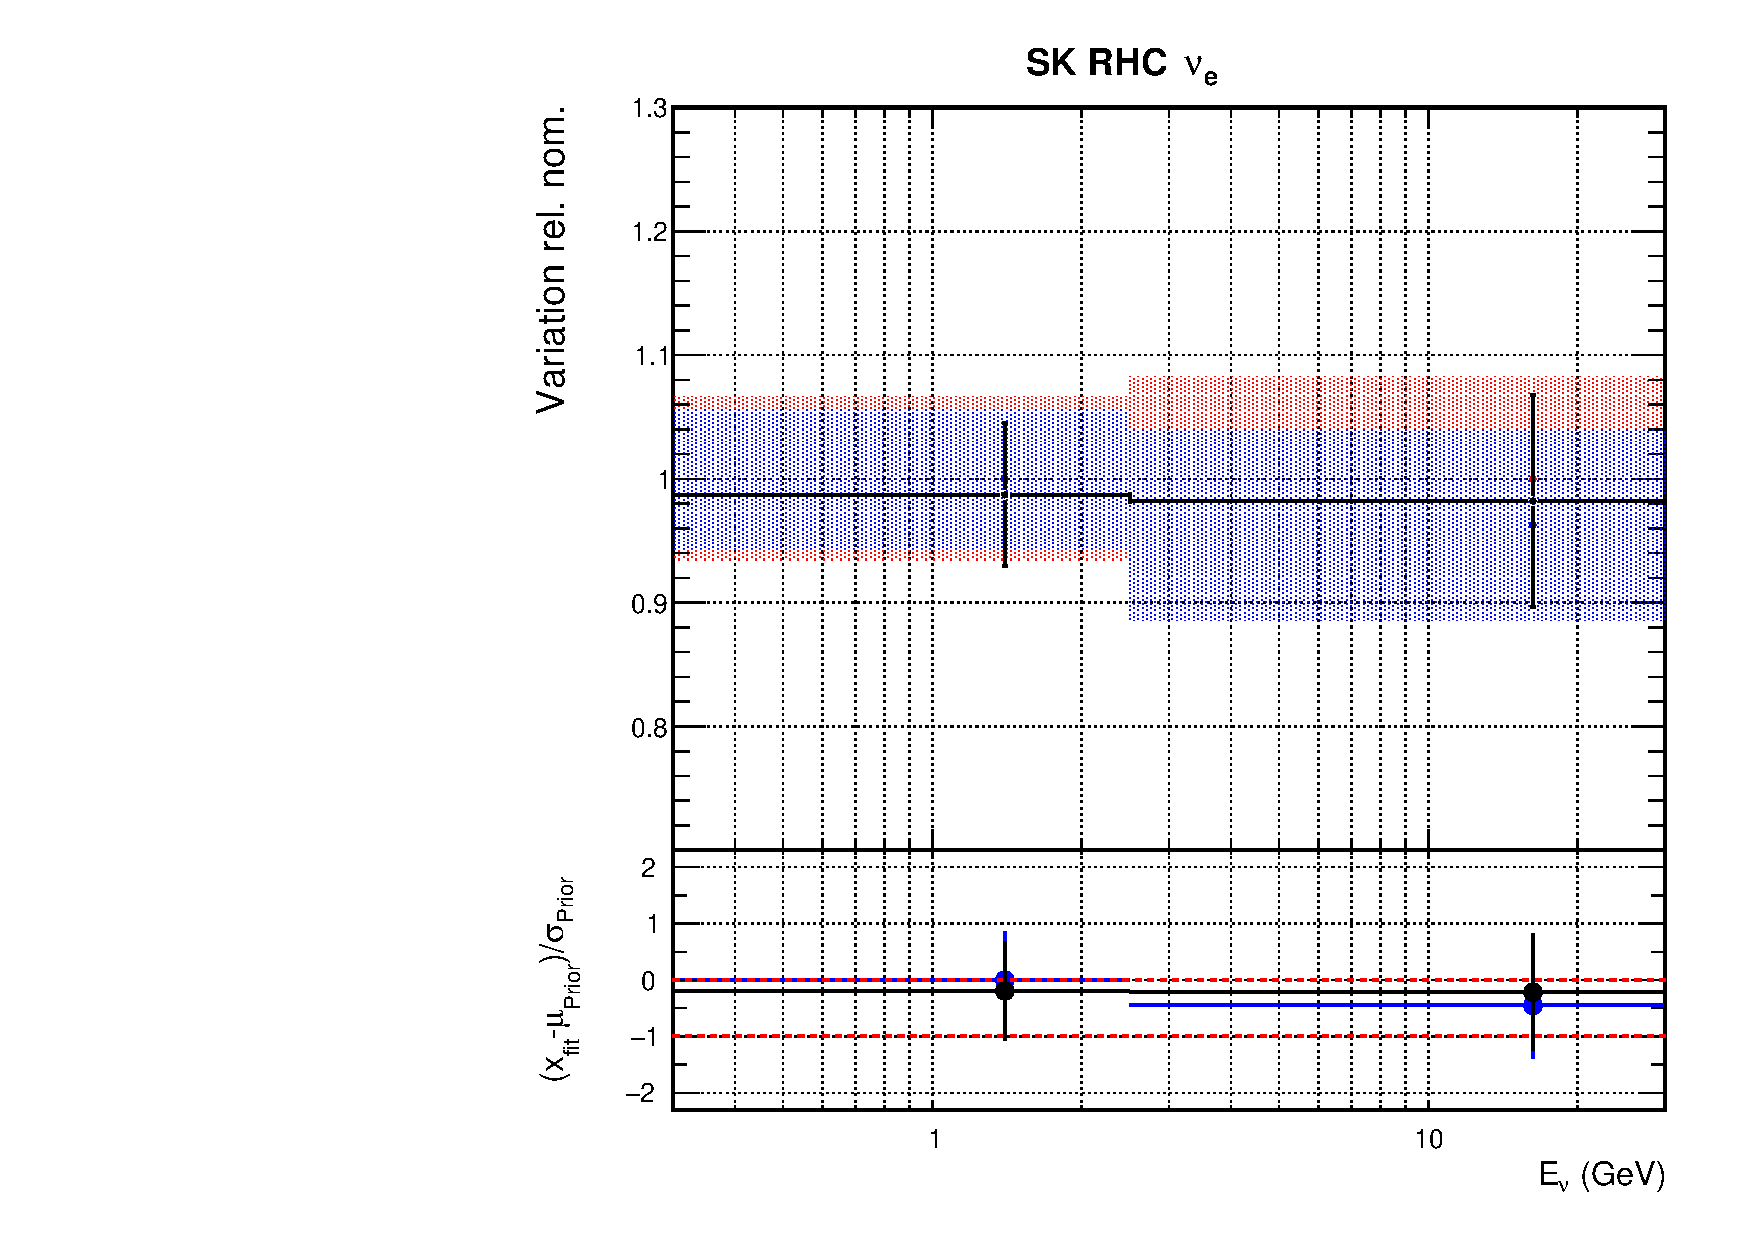
\includegraphics[width=0.95\linewidth]{figs/rhcmpasmvflux14}
  \caption{SK RHC $\nu_{\mu}$}
\end{subfigure}
\begin{subfigure}{0.24\textwidth}
  \centering
  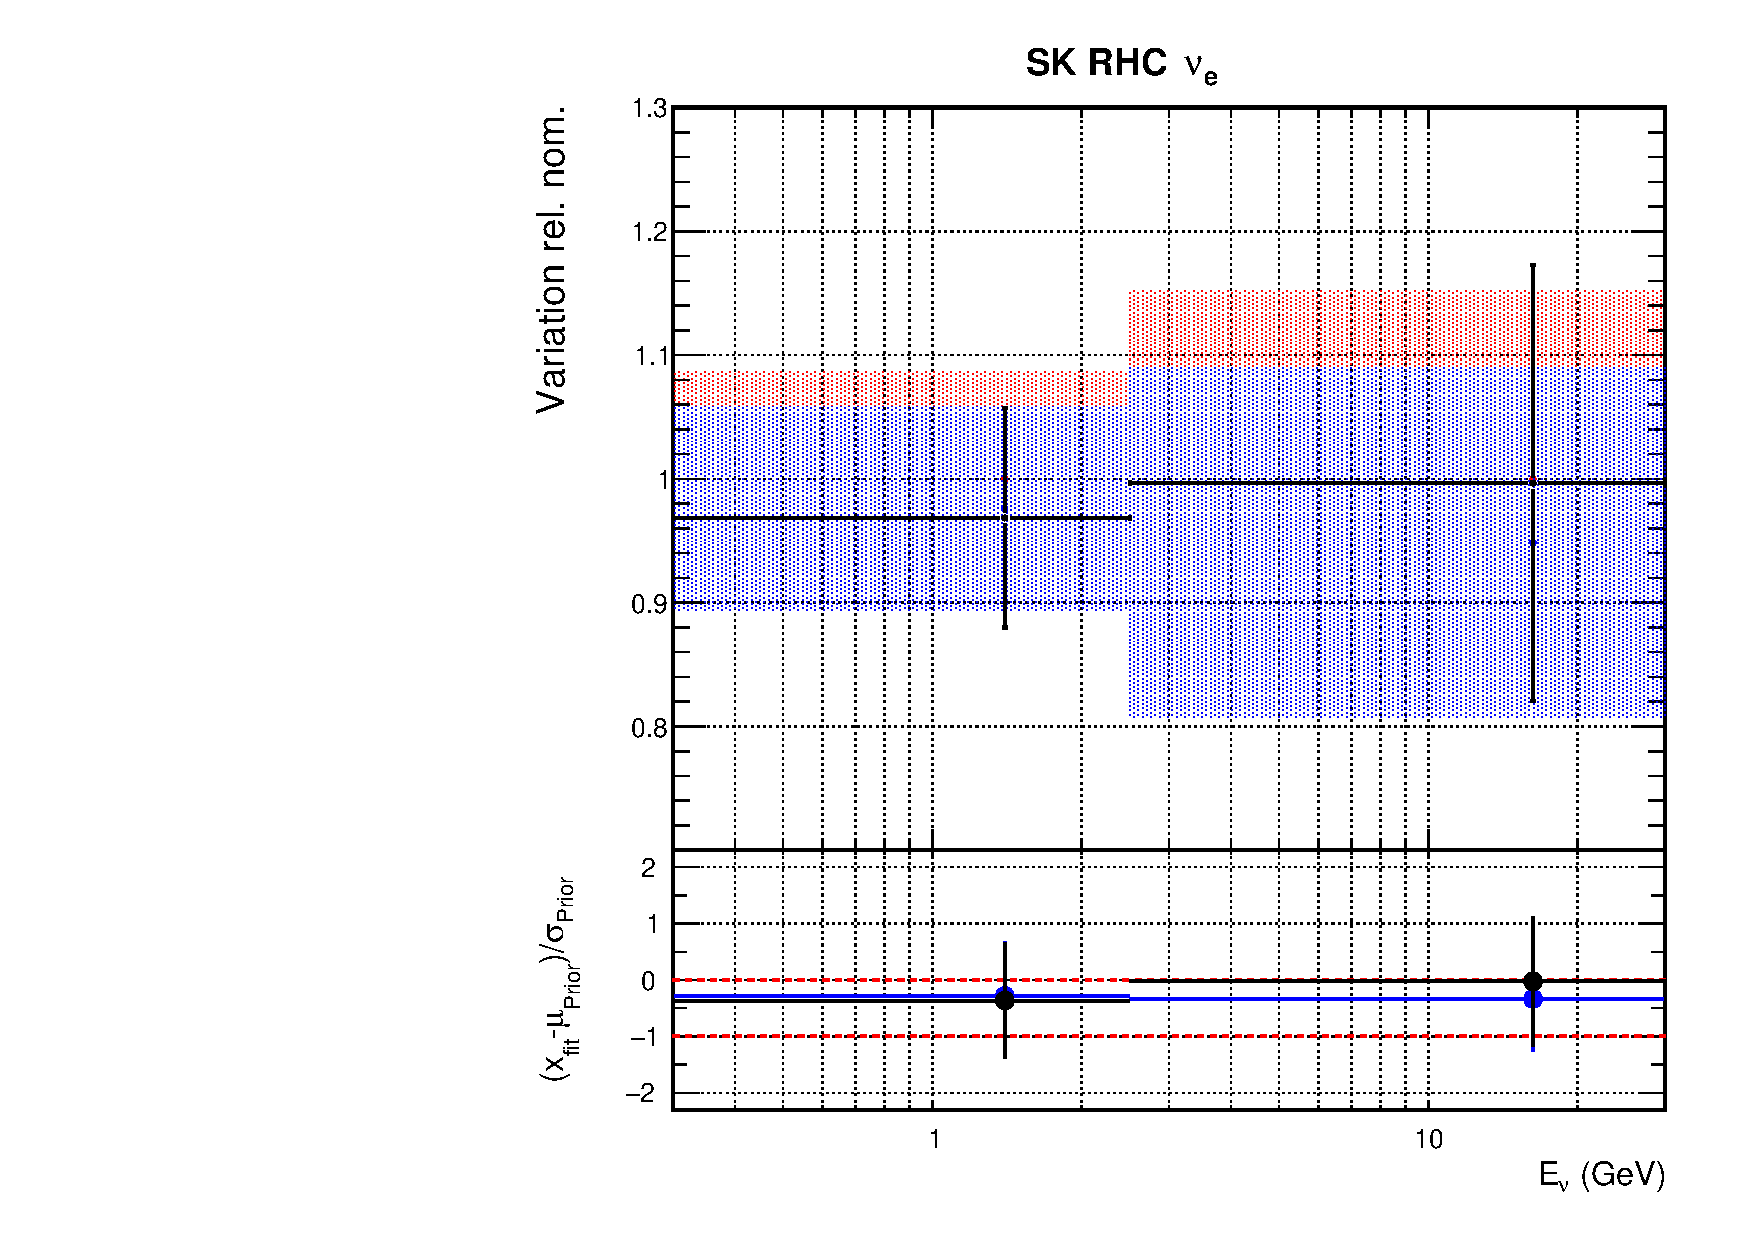
\includegraphics[width=0.95\linewidth]{figs/rhcmpasmvflux15}
  \caption{SK RHC $\nu_e$}
\end{subfigure}
\caption{Flux parameters for Asimov fits using FHC and RHC data.}
\label{fig:rhcmpiasmvSK}
\end{figure}

\begin{figure}[t]
\centering
\begin{subfigure}{0.95\textwidth}
  \centering
  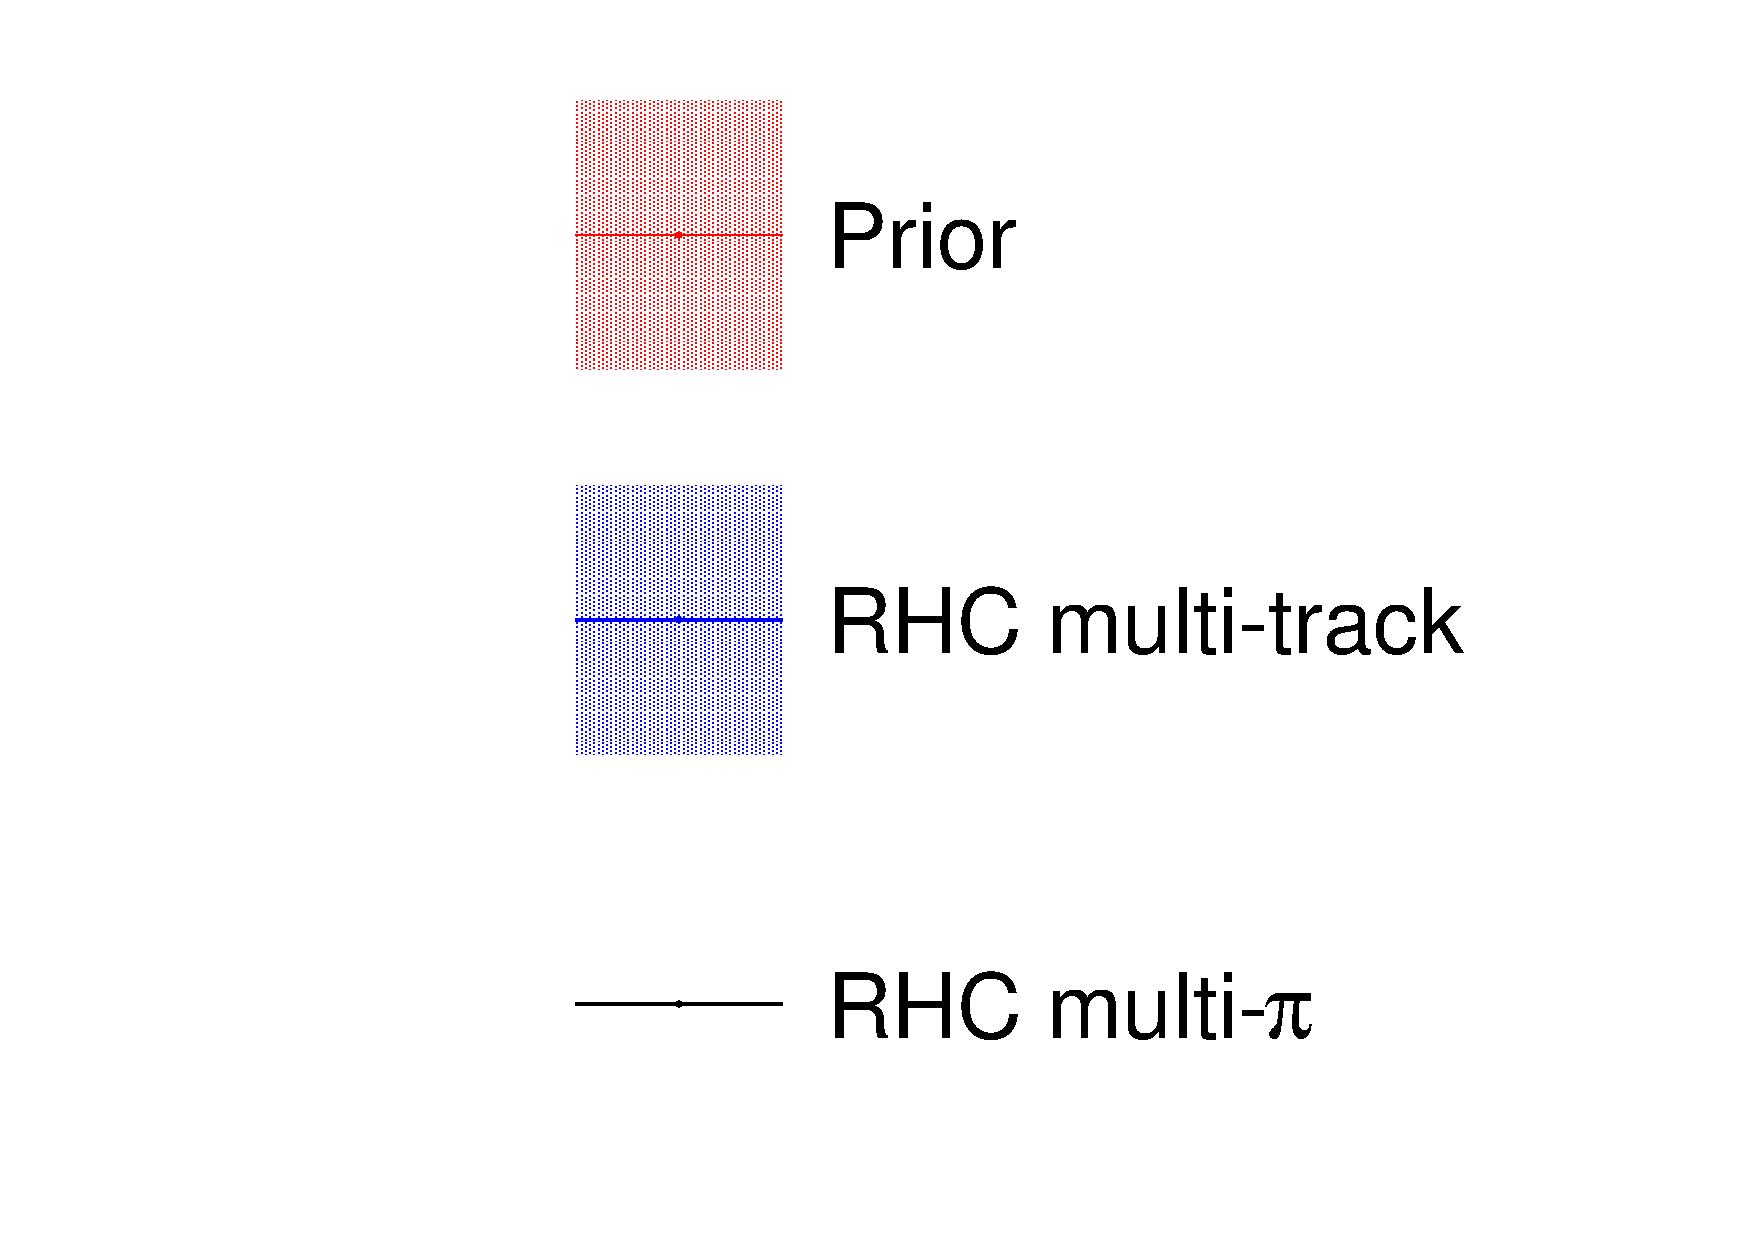
\includegraphics[width=0.25\linewidth]{figs/rhcmpasmv_leg}	
\end{subfigure}
\begin{subfigure}{0.49\textwidth}
  \centering
  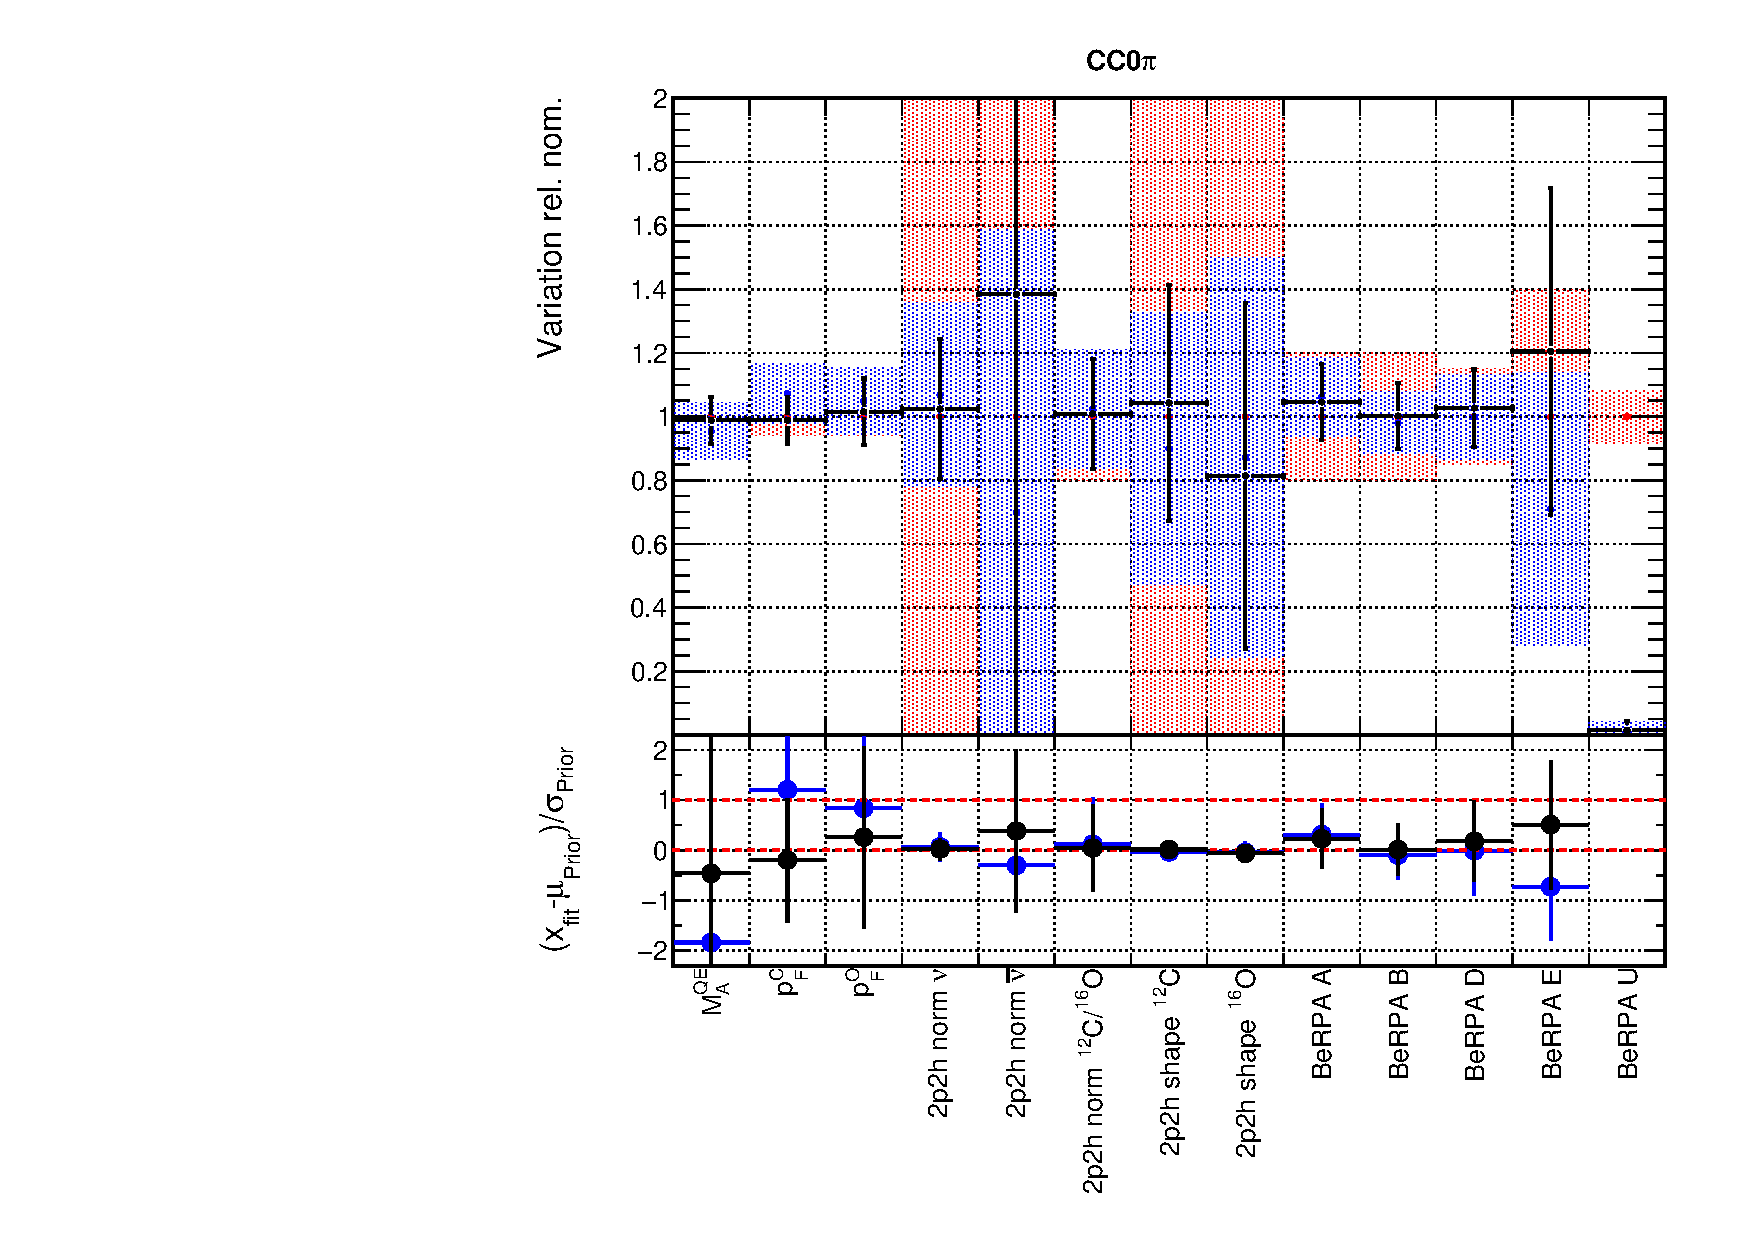
\includegraphics[width=0.95\linewidth]{figs/rhcmpasmvxsec1}
  \caption{CC0$\pi$}
\end{subfigure}
\begin{subfigure}{0.49\textwidth}
  \centering
  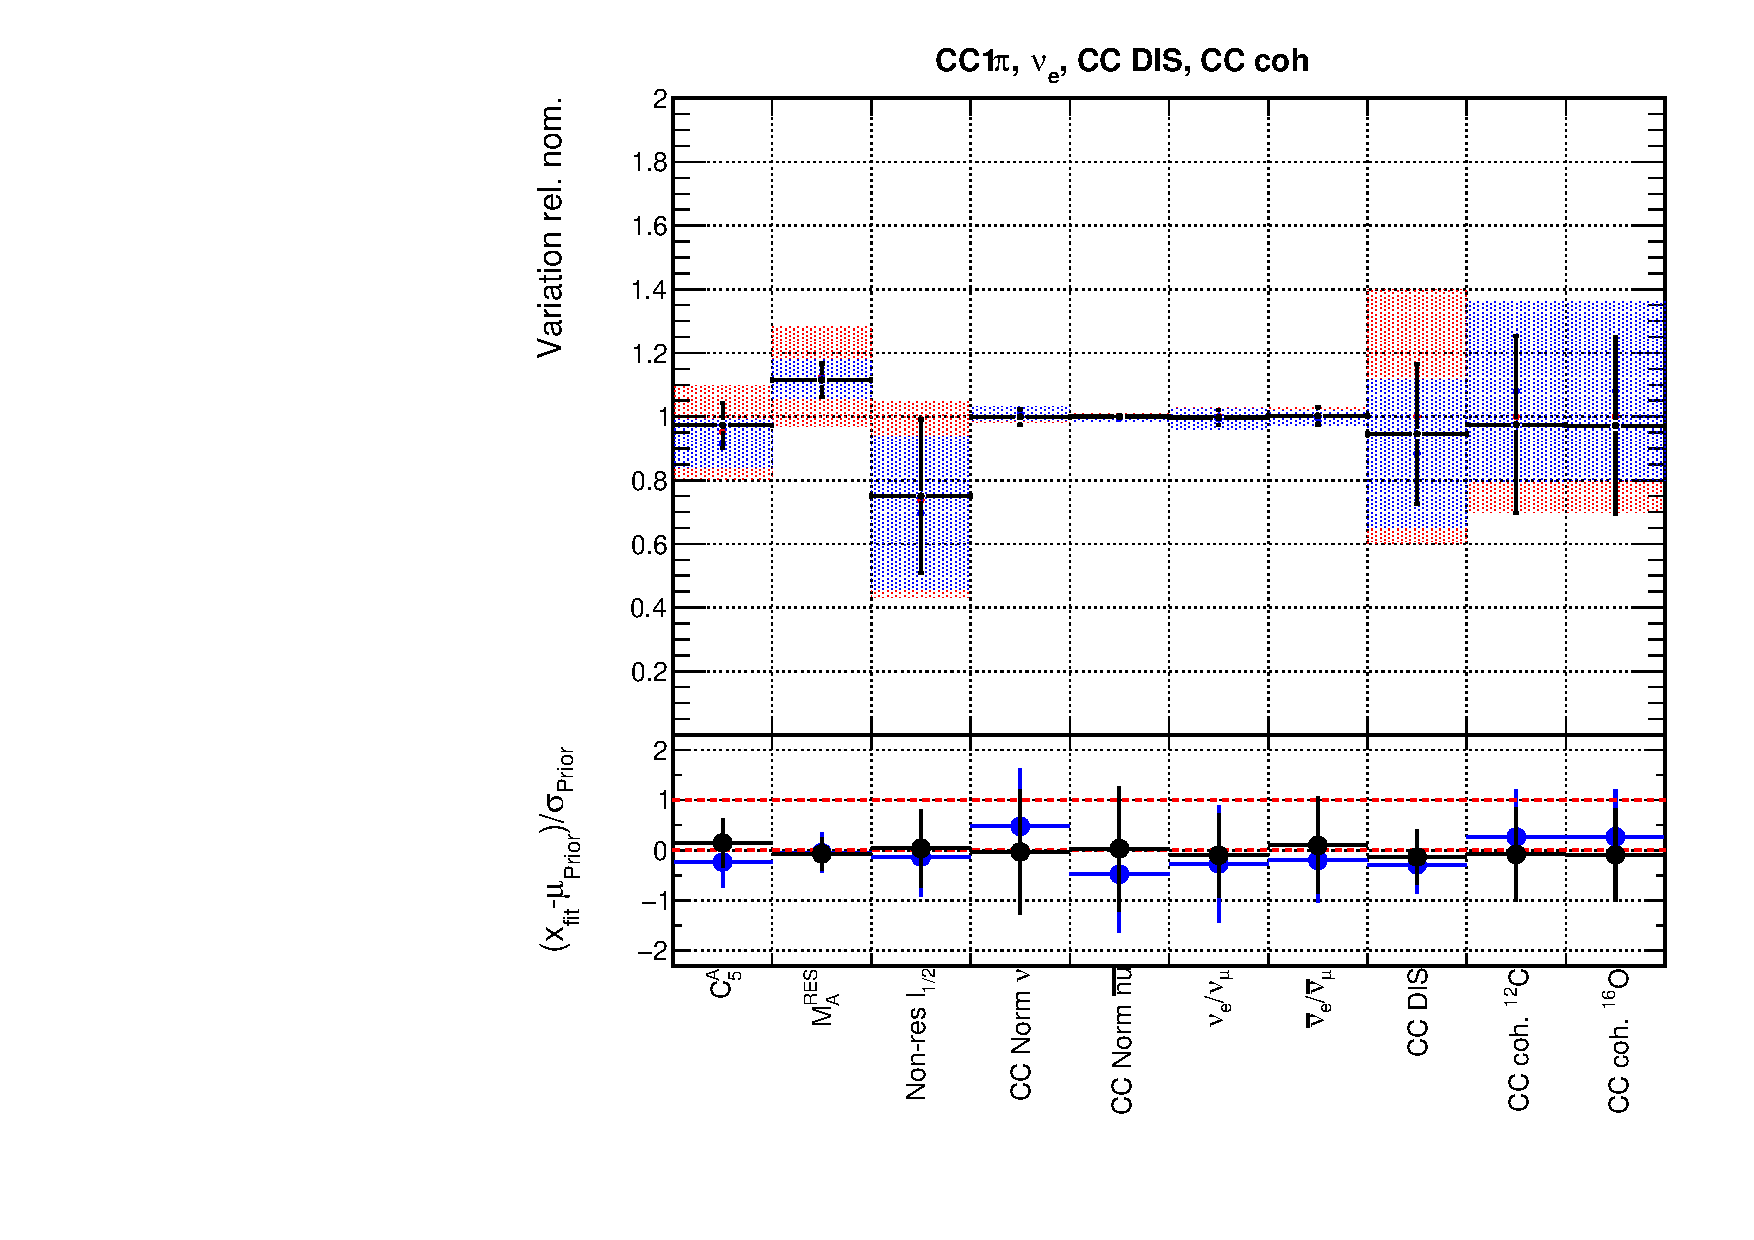
\includegraphics[width=0.95\linewidth]{figs/rhcmpasmvxsec2}
  \caption{CC1$\pi$, $\nu_e$, CC DIS, and CC coh.}
\end{subfigure}
\begin{subfigure}{0.49\textwidth}
  \centering
  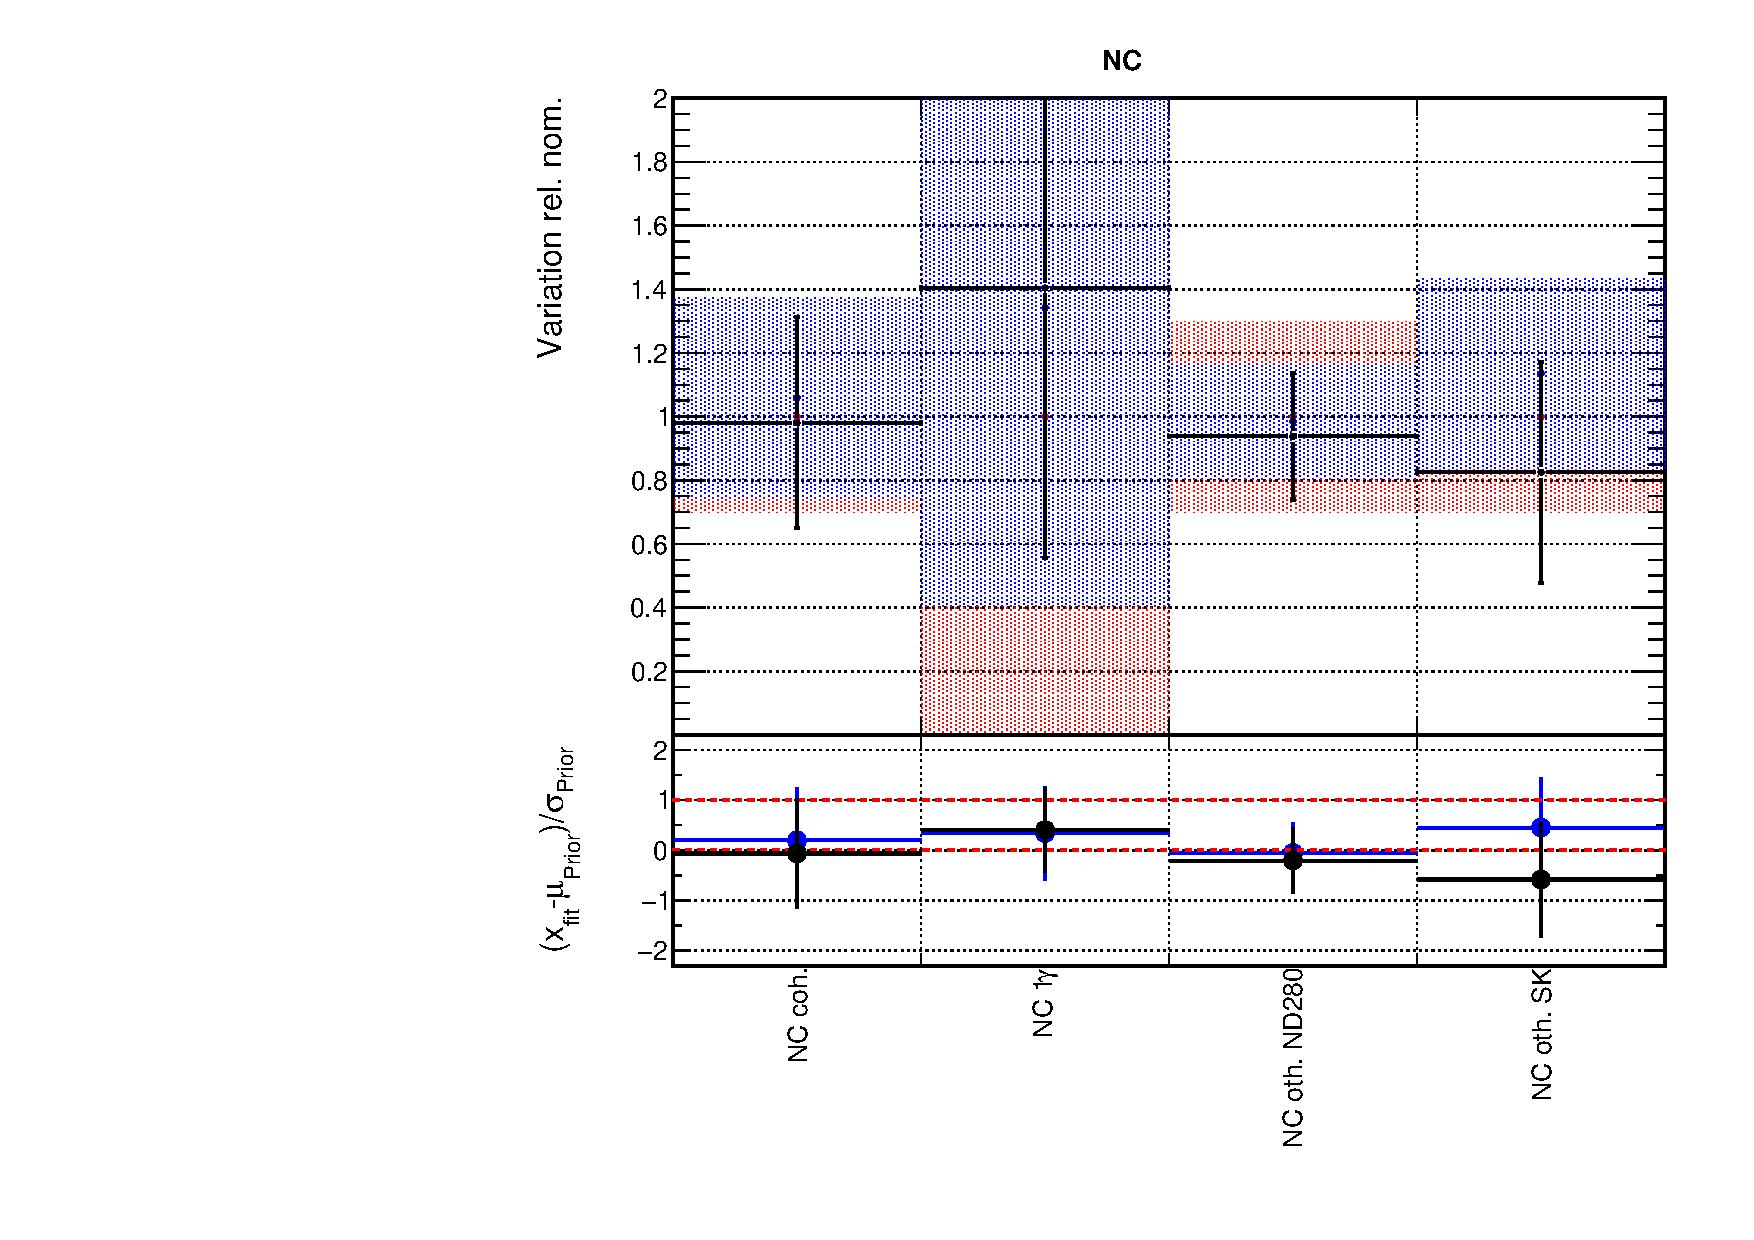
\includegraphics[width=0.95\linewidth]{figs/rhcmpasmvxsec3}
  \caption{NC}
\end{subfigure}
\begin{subfigure}{0.49\textwidth}
  \centering
  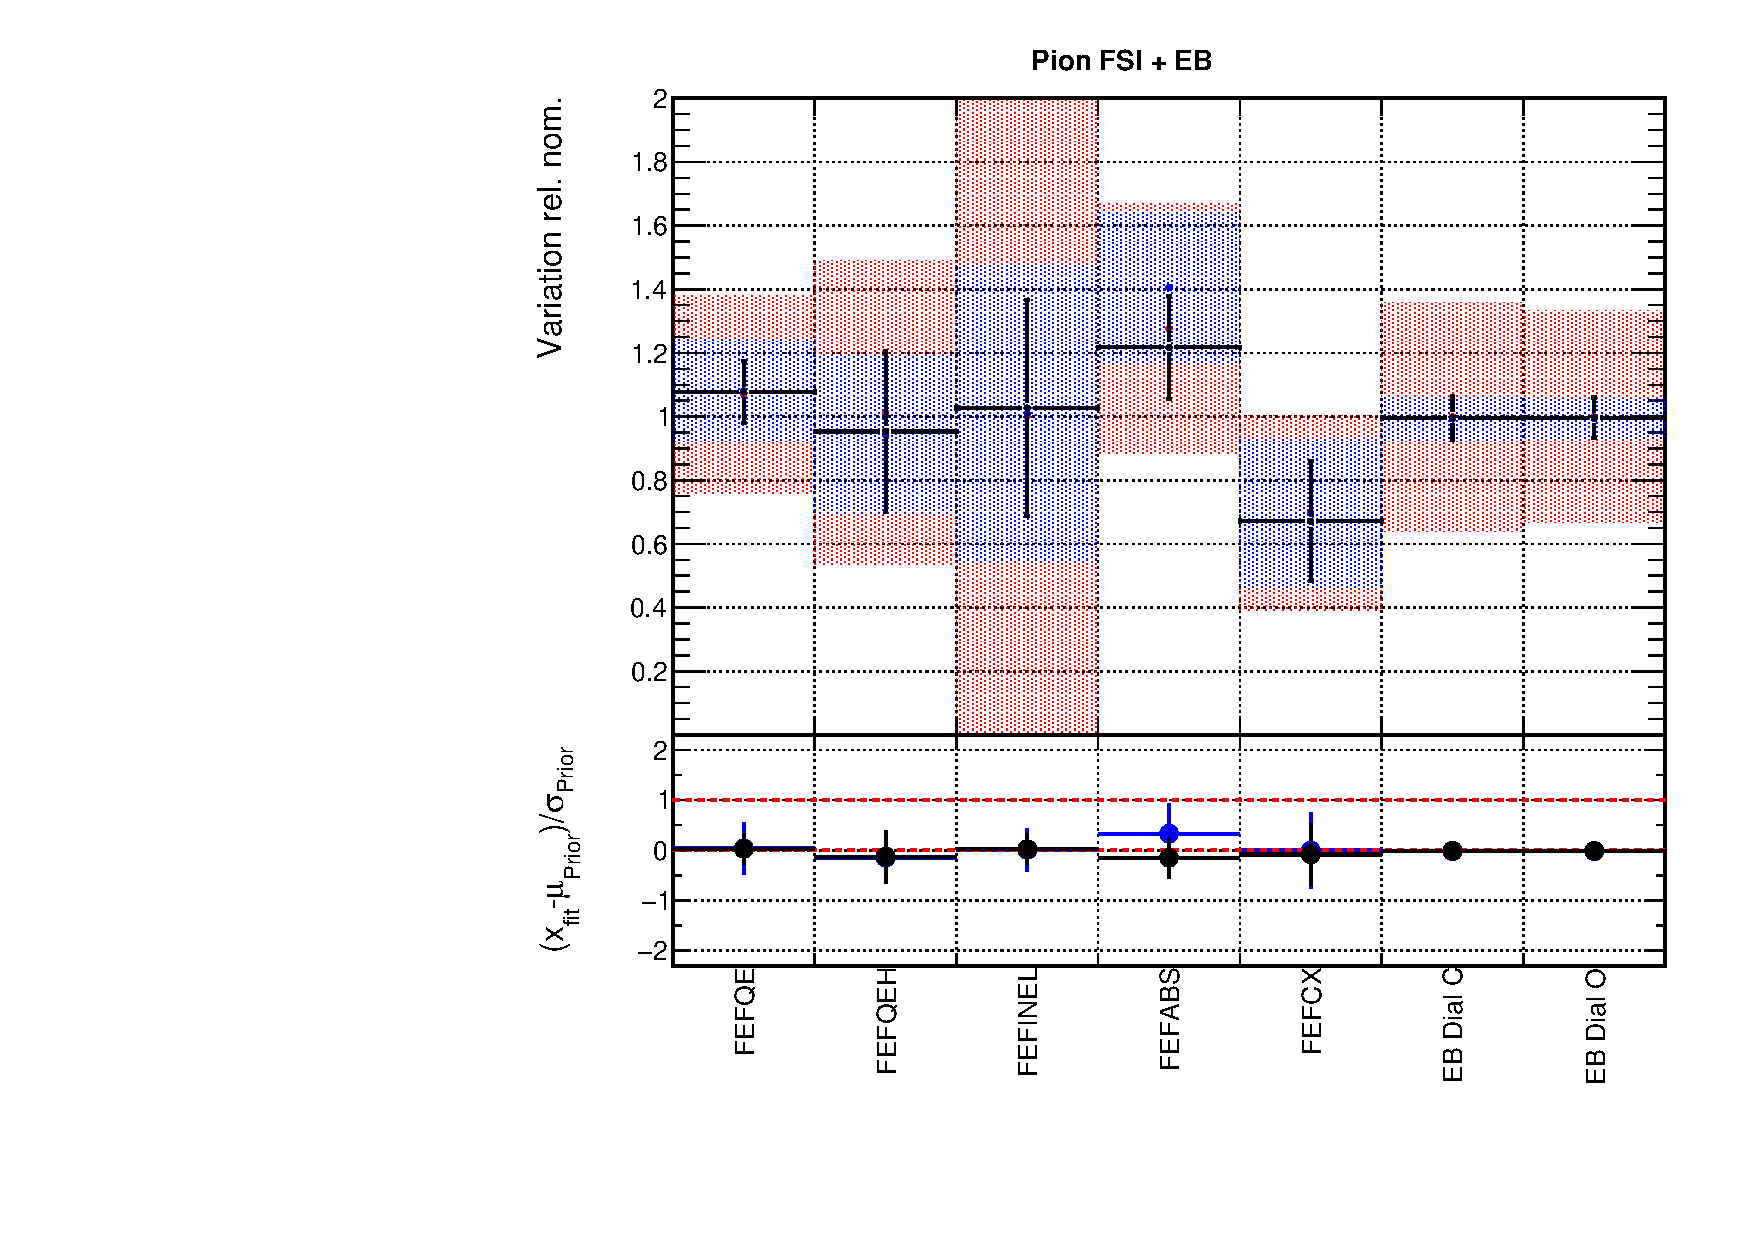
\includegraphics[width=0.95\linewidth]{figs/rhcmpasmvxsec4}
  \caption{$\pi$ FSI and $E_b$}
\end{subfigure}
\caption{Interaction parameters for Asimov fits using FHC and RHC data.}
\label{fig:rhcmpiasmvxsec}
\end{figure}

The data fits using both FHC and RHC data have more differences. The flux parameters, shown in Figure \ref{fig:rhcmpidat28SK}, are pulled further from nominal at low energies. The oscillatory shape of the pulls in energy are similar for the two selections, and postfit values are consistently within 1$\sigma$ of each other. The ND and SK flux parameters have similar behaviour.
 
The interaction parameters, shown in \ref{fig:rhcmpidat28xsec}, also have fairly significant differences. The 2p2h normalisations for $\nu$ and $\bar{\nu}$ are both closer to nominal using the mulit-$\pi$ samples, whereas the 2p2h shape parameter on C is pulled about 1$\sigma$ further. The CC1$\pi$ parameters are very compatible for the two selections, but the CC DIS parameter is closer to nominal for the mulit-$\pi$ samples. The NC Other (NC1$\pi$ and NC DIS) is the only NC parameter to show any differences, being pulled $>1\sigma$ higher. For the $\pi$ FSI parameters, the high energy quasi-elastic and $\pi$ absorption parameters are closer to nominal, whereas the charge exchange parameter is pulled further away for the mulit-$\pi$ samples.

Overall the fits are largely compatible, with parameters mostly being within 1$\sigma$ for the two selections, and often being closer to nominal for multi-$\pi$.

\begin{figure}[t]
\centering
\begin{subfigure}{0.95\textwidth}
  \centering
  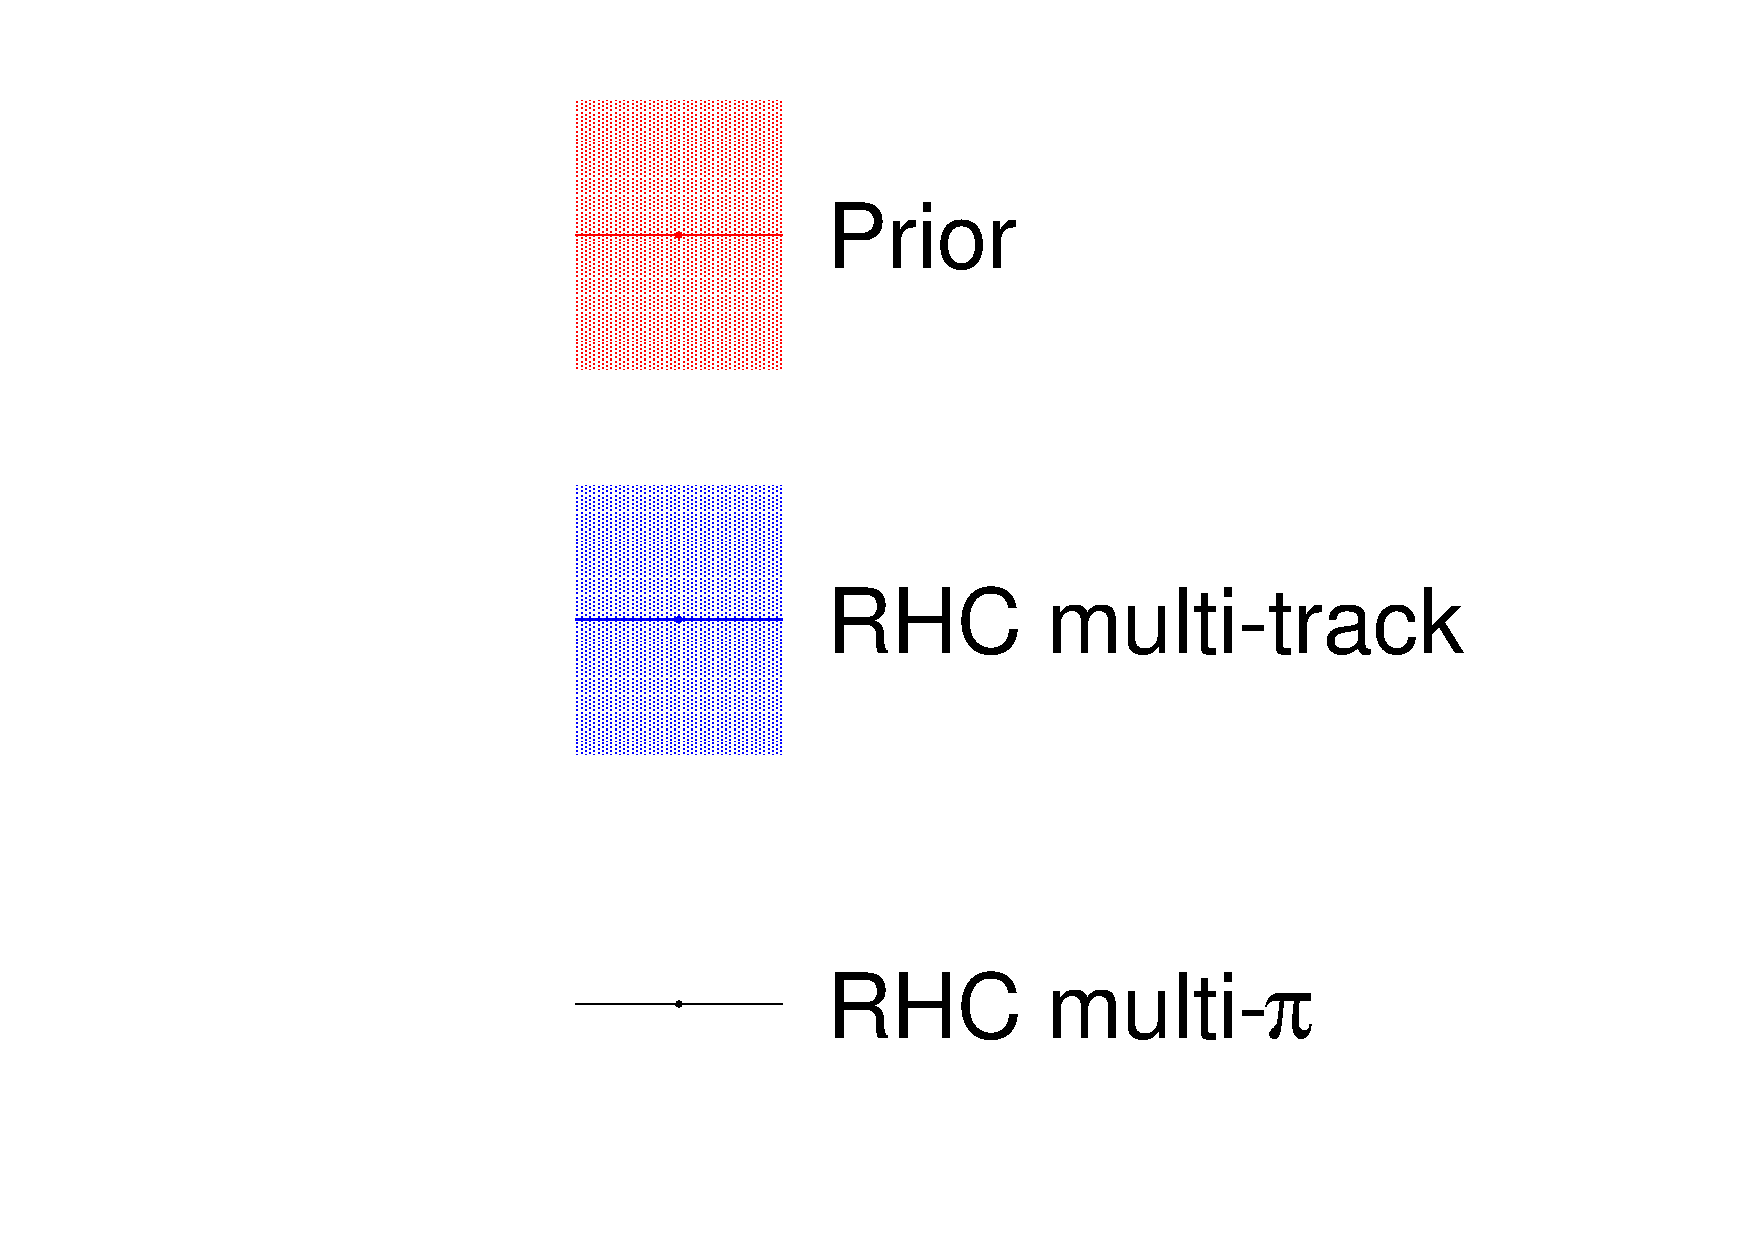
\includegraphics[width=0.24\linewidth]{figs/rhcmpdat28_leg}	
\end{subfigure}
\begin{subfigure}{0.24\textwidth}
  \centering
  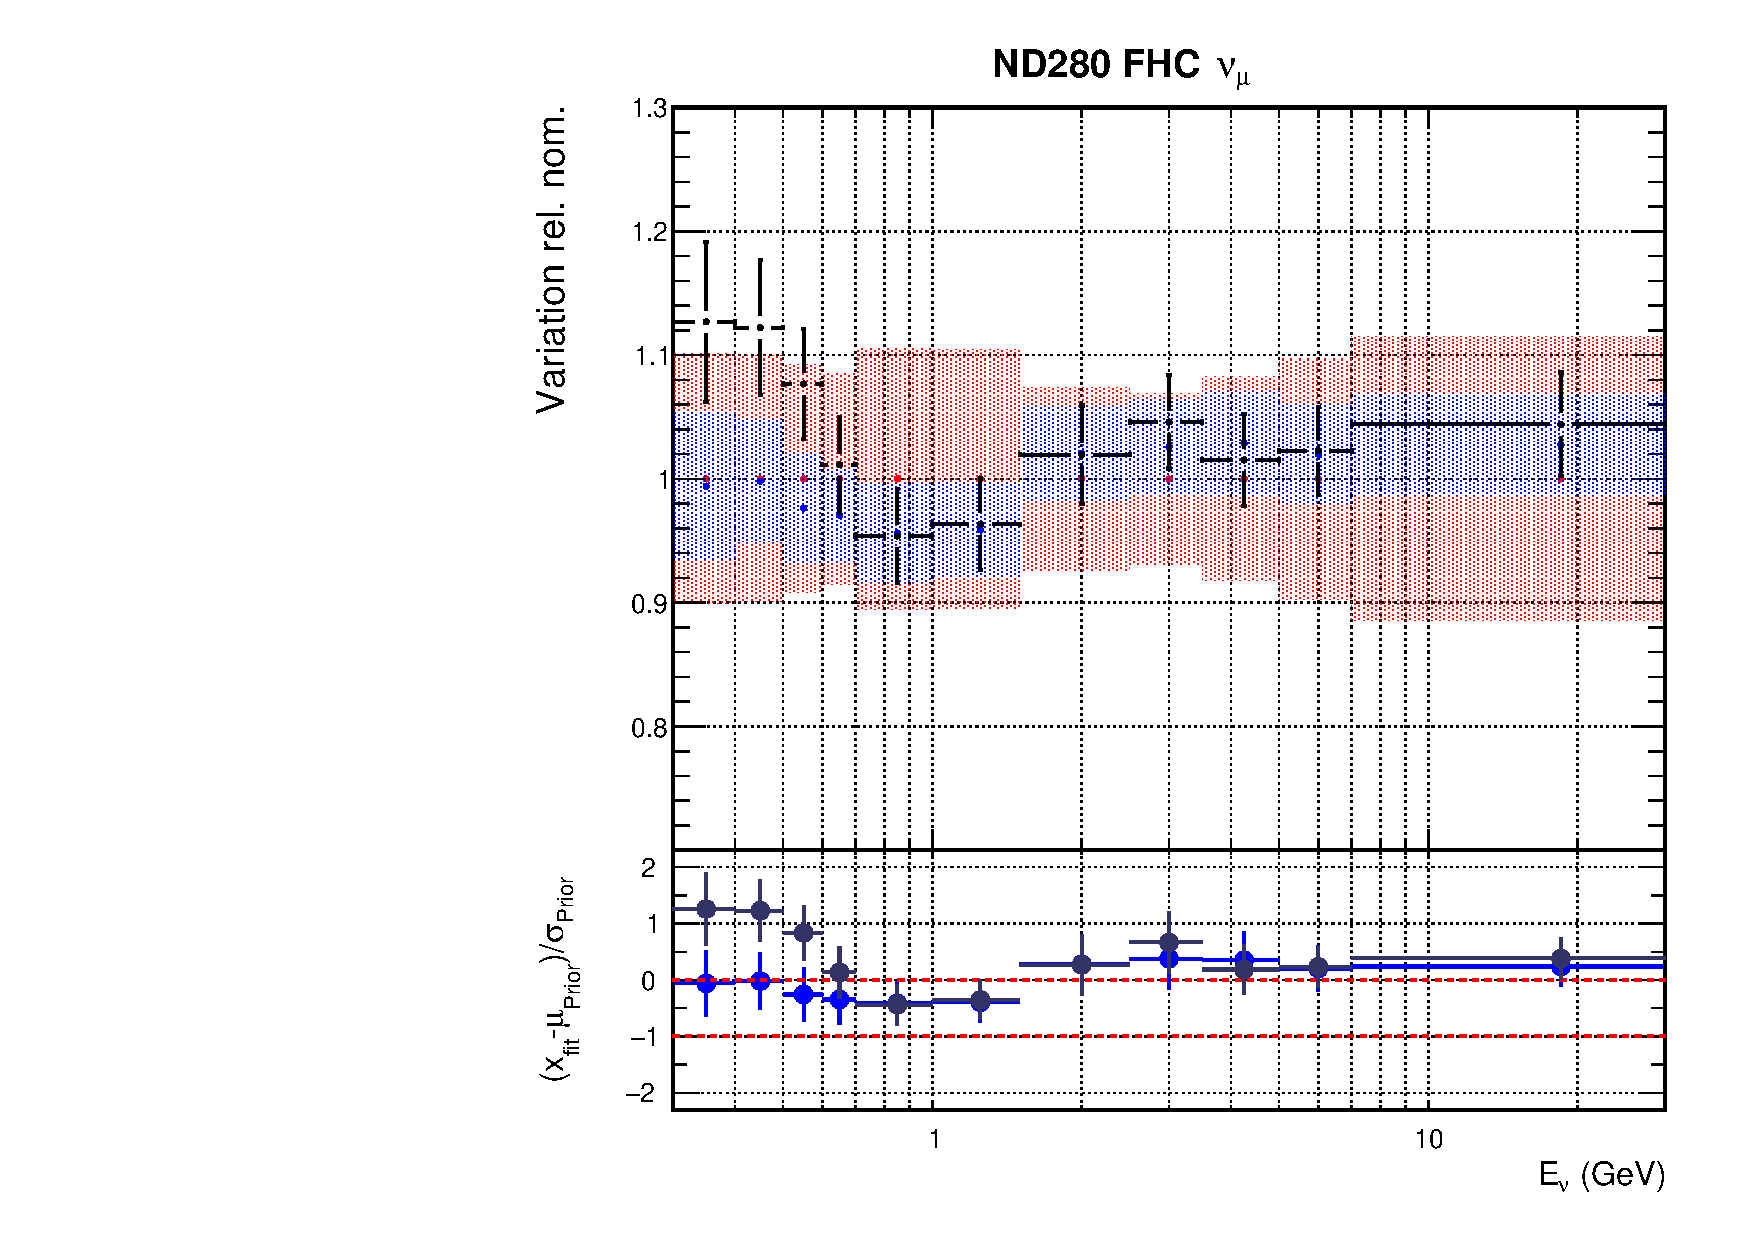
\includegraphics[width=0.95\linewidth]{figs/rhcmpdat28flux_0}
  \caption{ND FHC $\nu_{\mu}$}
\end{subfigure}
\begin{subfigure}{0.24\textwidth}
  \centering
  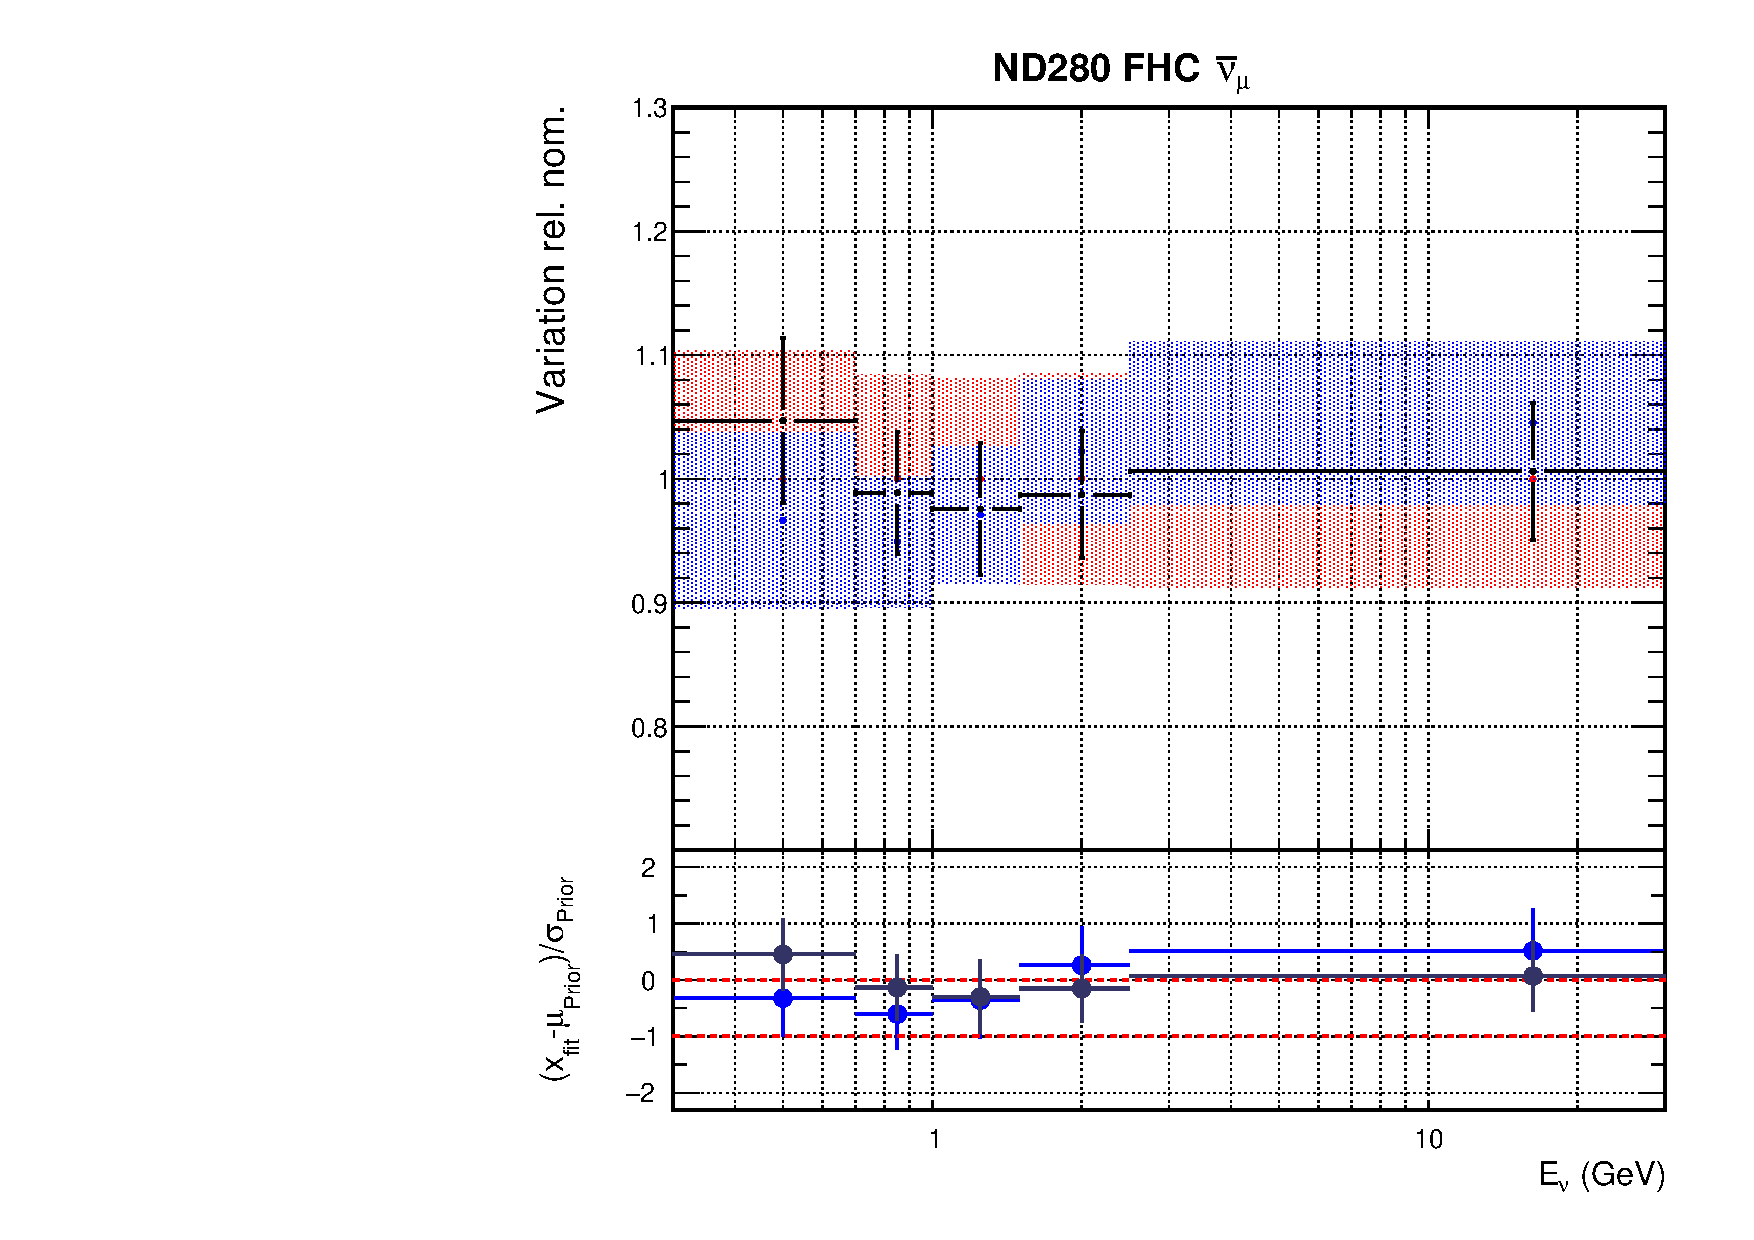
\includegraphics[width=0.95\linewidth]{figs/rhcmpdat28flux_1}
  \caption{ND FHC $\nu_{e}$}
\end{subfigure}
\begin{subfigure}{0.24\textwidth}
  \centering
  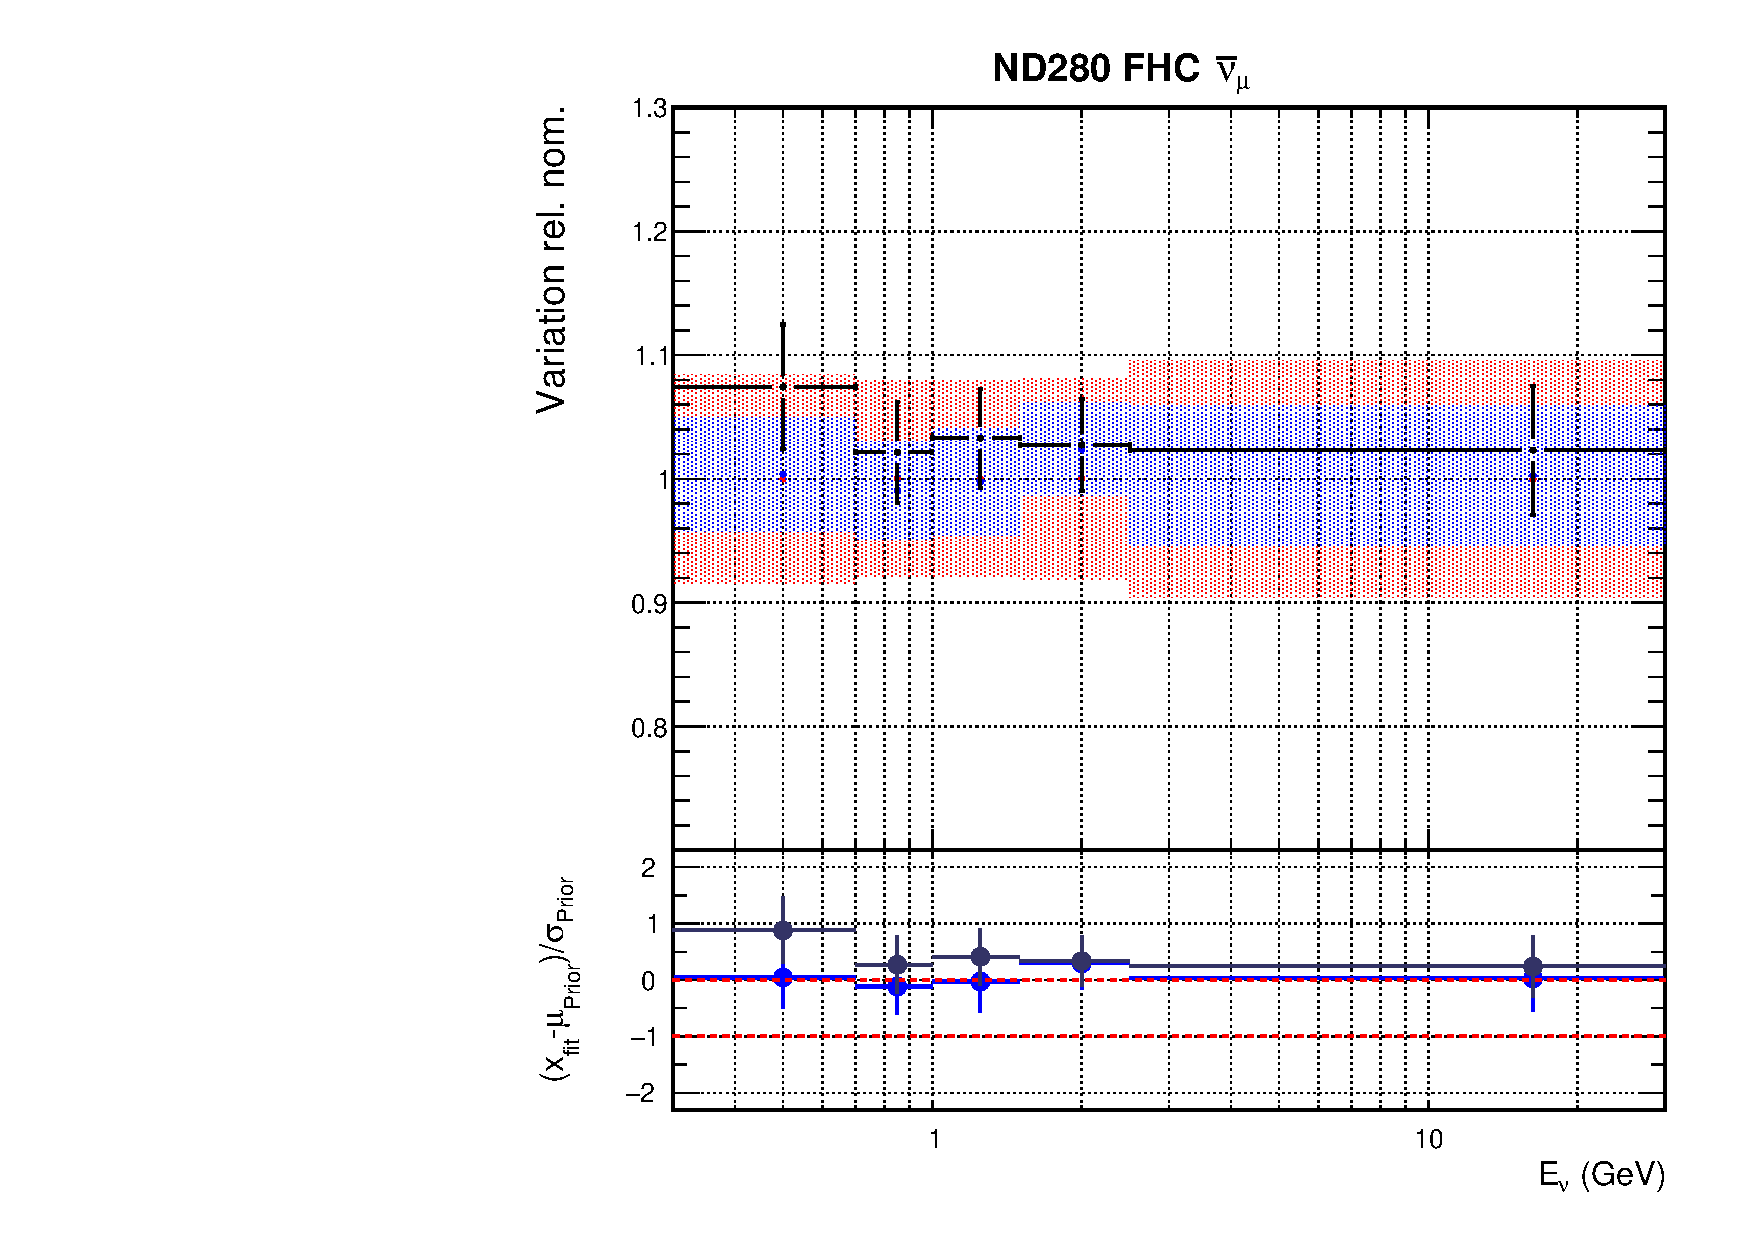
\includegraphics[width=0.95\linewidth]{figs/rhcmpdat28flux_2}
  \caption{ND FHC $\bar{\nu_{\mu}}$}
\end{subfigure}
\begin{subfigure}{0.24\textwidth}
  \centering
  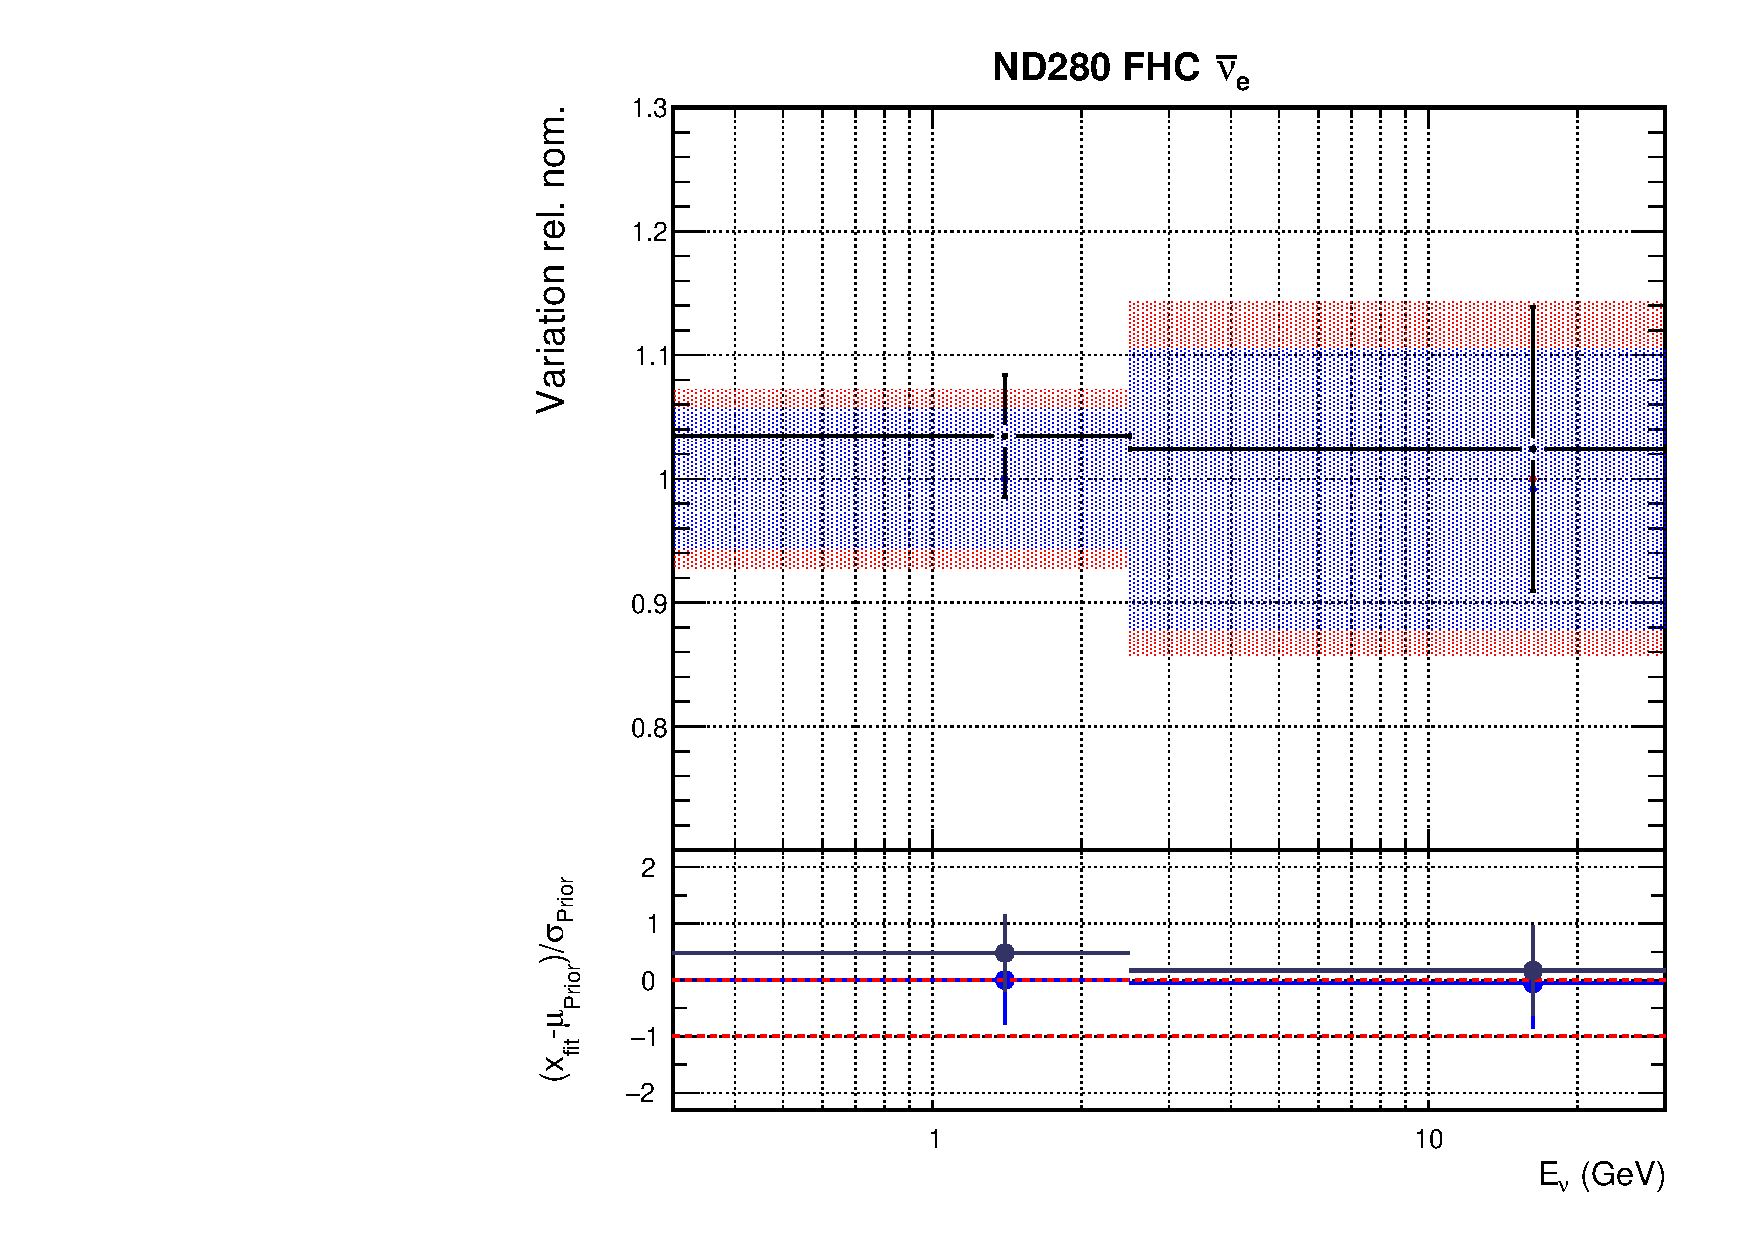
\includegraphics[width=0.95\linewidth]{figs/rhcmpdat28flux_3}
  \caption{ND FHC $\bar{\nu_{e}}$}
\end{subfigure}
\begin{subfigure}{0.24\textwidth}
  \centering
  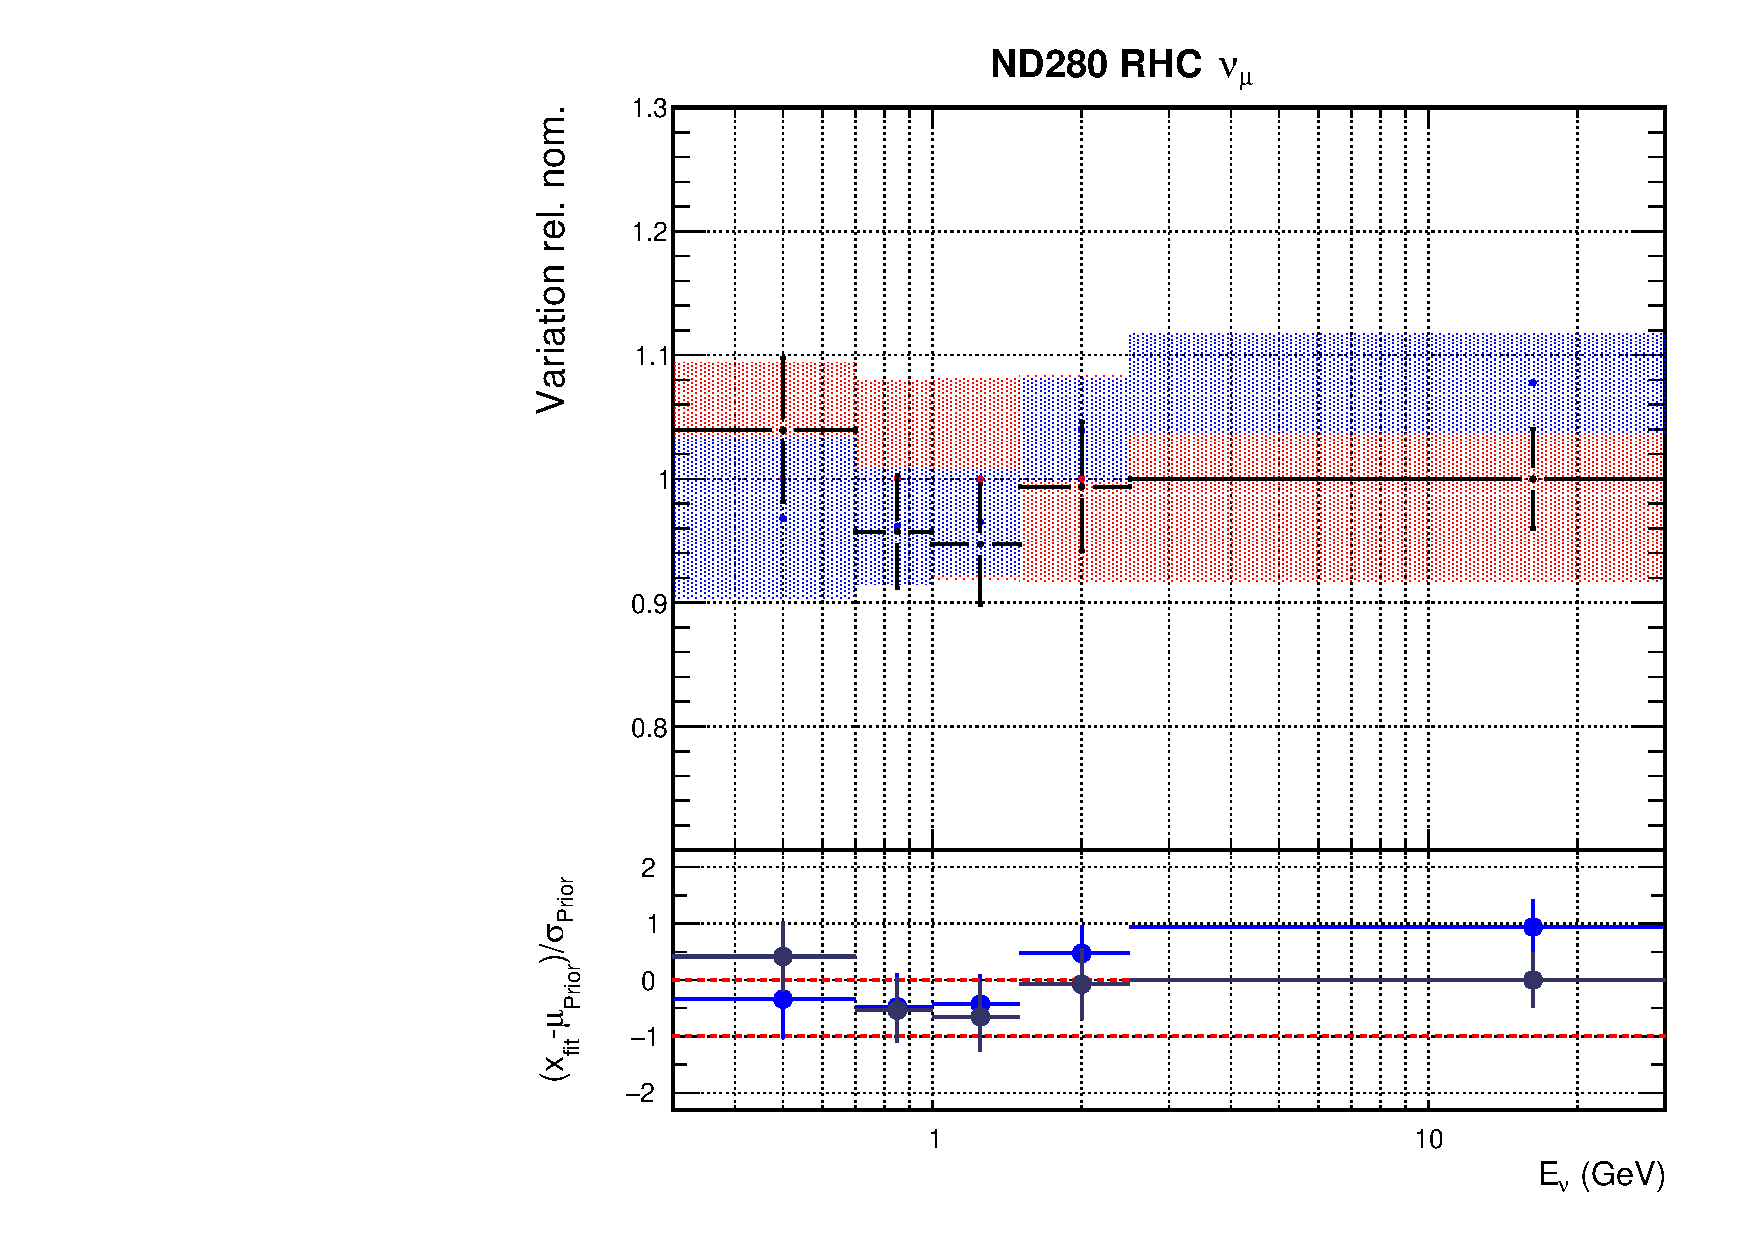
\includegraphics[width=0.95\linewidth]{figs/rhcmpdat28flux_4}
  \caption{ND RHC $\bar{\nu_{\mu}}$}
\end{subfigure}
\begin{subfigure}{0.24\textwidth}
  \centering
  \includegraphics[width=0.95\linewidth]{figs/rhcmpdat28flux_5}
  \caption{ND RHC $\bar{\nu_e}$}
\end{subfigure}
\begin{subfigure}{0.24\textwidth}
  \centering
  \includegraphics[width=0.95\linewidth]{figs/rhcmpdat28flux_6}
  \caption{ND RHC $\nu_{\mu}$}
\end{subfigure}
\vspace{15mm}
\begin{subfigure}{0.24\textwidth}
  \centering
  \includegraphics[width=0.95\linewidth]{figs/rhcmpdat28flux_7}
  \caption{ND RHC $\nu_e$}
\end{subfigure}
\begin{subfigure}{0.24\textwidth}
  \centering
  \includegraphics[width=0.95\linewidth]{figs/rhcmpdat28flux_8}
  \caption{SK FHC $\nu_{\mu}$}
\end{subfigure}
\begin{subfigure}{0.24\textwidth}
  \centering
  \includegraphics[width=0.95\linewidth]{figs/rhcmpdat28flux_9}
  \caption{SK FHC $\nu_e$}
\end{subfigure}
\begin{subfigure}{0.24\textwidth}
  \centering
  \includegraphics[width=0.95\linewidth]{figs/rhcmpdat248flux_10}
  \caption{SK FHC $\bar{\nu_{\mu}}$}
\end{subfigure}
\begin{subfigure}{0.24\textwidth}
  \centering
  \includegraphics[width=0.95\linewidth]{figs/rhcmpdat28flux_11}
  \caption{SK FHC $\bar{\nu_{e}}$}
\end{subfigure}
\begin{subfigure}{0.24\textwidth}
  \centering
  \includegraphics[width=0.95\linewidth]{figs/rhcmpdat28flux_12}
  \caption{SK RHC $\bar{\nu_{\mu}}$}
\end{subfigure}
\begin{subfigure}{0.24\textwidth}
  \centering
  \includegraphics[width=0.95\linewidth]{figs/rhcmpdat28flux_13}
  \caption{SK RHC $\bar{\nu_{e}}$}
\end{subfigure}
\begin{subfigure}{0.24\textwidth}
  \centering
  \includegraphics[width=0.95\linewidth]{figs/rhcmpdat28flux_14}
  \caption{SK FHC $\nu_{\mu}$}
\end{subfigure}
\begin{subfigure}{0.24\textwidth}
  \centering
  \includegraphics[width=0.95\linewidth]{figs/rhcmpdat28flux_15}
  \caption{SK RHC $\nu_{e}$}
\end{subfigure}
\caption{Flux parameters for data fits using FHC and RHC data.}
\label{fig:rhcmpidat28SK}
\end{figure}

\begin{figure}[t]
\centering
\begin{subfigure}{0.95\textwidth}
  \centering
  \includegraphics[width=0.25\linewidth]{figs/rhcmpdat28_leg}	
\end{subfigure}
\begin{subfigure}{0.49\textwidth}
  \centering
  \includegraphics[width=0.95\linewidth]{figs/rhcmpdatxsec28_1}
  \caption{CC0$\pi$}
\end{subfigure}
\begin{subfigure}{0.49\textwidth}
  \centering
  \includegraphics[width=0.95\linewidth]{figs/rhcmpdatxsec28_2}
  \caption{CC1$\pi$, $\nu_e$, CC DIS, and CC coh}
\end{subfigure}
\begin{subfigure}{0.49\textwidth}
  \centering
  \includegraphics[width=0.95\linewidth]{figs/rhcmpdatxsec28_3}
  \caption{NC}
\end{subfigure}
\begin{subfigure}{0.49\textwidth}
  \centering
  \includegraphics[width=0.95\linewidth]{figs/rhcmpdatxsec28_4}
  \caption{$\pi$ FSI and $E_b$}
\end{subfigure}
\caption{Interaction parameters for data fits using FHC and RHC data.}
\label{fig:rhcmpidat28xsec}
\end{figure}

These validation fits were run using an intermediate cross-section model made up of the one used for the 2017 oscillation analysis, which is described in more detail in \cite{tn315}, plus normalisations for the CC $\nu$ and $\bar{\nu}$ cross-section, Coulomb corrections, and binding energy dials. 

\newpage
